\documentclass[twocolumn,floatfix,showpacs,rmp,aps]{revtex4}
%\documentclass[rmp,aps,preprint,showpacs,floatfix]{revtex4}
\pdfoutput=1
\usepackage{amssymb}
\usepackage{amsmath}
\usepackage{bm}
\usepackage[pdftex]{graphicx}

\begin{document}
	\title{Topological Insulators}
	
	\author{M. Z. Hasan}
	\email{mzhasan@princeton.edu}
	\affiliation{Joseph Henry Laboratories, Department of Physics,
		Princeton University, Princeton, NJ 08544}
	
	\author{C. L. Kane}
	\email{kane@physics.upenn.edu}
	\affiliation{Department of Physics and Astronomy,
		University of Pennsylvania, Philadelphia, PA 19104}
	
	\begin{abstract}
		Topological insulators are electronic materials that
		have a bulk band gap like an ordinary insulator, but have protected conducting
		states on their edge or surface.  These states are possible due to the combination of spin orbit
		interactions and time reversal symmetry.  The 2D topological insulator is a
		quantum spin Hall insulator, which is a close cousin of the integer
		quantum Hall state. A 3D topological
		insulator supports novel spin polarized 2D Dirac fermions on its surface.  In this
		Colloquium article we will review the theoretical foundation for
		topological insulators and superconductors and describe recent experiments in which
		the signatures of topological insulators have been observed.  We will describe transport
		experiments on HgTe/CdTe quantum wells that demonstrate the
		existence of the edge states predicted for the quantum spin Hall
		insulator. We will then discuss experiments on Bi$_{1-x}$Sb$_x$, Bi$_2$Se$_3$,
		Bi$_2$Te$_3$ and Sb$_2$Te$_3$ that establish these materials as 3D topological
		insulators and directly probe the topology of their surface states.
		We will then describe exotic
		states that can occur at the surface of a 3D topological
		insulator due to an induced energy gap.  A magnetic gap leads to a
		novel quantum Hall state that gives rise to a topological
		magnetoelectric effect.  A superconducting energy gap leads to a
		state that supports Majorana fermions, and may provide a new venue
		for realizing proposals for topological quantum computation.  We will
		close by discussing prospects for observing these exotic states, as
		well as other potential device applications of topological
		insulators.
	\end{abstract}
	
	\pacs{73.20.-r, 73.43.-f, 85.75.-d, 74.90.+n}
	%\date{May 2001}
	\maketitle
	\tableofcontents
	
	\section{Introduction}
	\label{sec:intro}
	
	A recurring theme in condensed matter physics
	has been the discovery and classification of distinctive phases of matter.
	Often, phases can be understood using Landau's approach, which characterizes
	states in terms of underlying symmetries that are spontaneously
	broken.   Over the past 30 years, the study
	of the quantum Hall effect has led to a different classification paradigm, based
	on the notion of {\it topological order} \cite{thouless82,wen95}.  The
	state responsible for the quantum Hall effect does not
	break any symmetries, but it defines a topological phase in the
	sense that certain fundamental properties (such as the quantized value of the
	Hall conductance, and the number of gapless boundary modes)
	are insensitive to smooth changes in materials
	parameters and can not change unless the system passes
	through a quantum phase transition.
	
	In the past five years a new field has emerged in condensed matter
	physics, based on the realization that the spin orbit interaction can
	lead to topological insulating electronic phases
	\cite{kanemele05a,kanemele05b,moorebalents07,fukanemele07,roy09b}, and on the prediction
	and observation of these phases in real materials
	\cite{bernevighugheszhang06,fukane07,konig07,hsieh08,xia09a,zhangh09}.  A
	topological insulator, like an ordinary insulator, has a bulk energy
	gap separating the highest occupied electronic band from the lowest
	empty band. The surface (or edge in two dimensions) of a topological
	insulator, however, necessarily has gapless states that are
	protected by time reversal symmetry.  The
	topological insulator is closely related to the two dimensional (2D)
	integer quantum Hall state, which also has unique
	edge states.   The surface (or edge) states of a topological insulator lead
	to a conducting state with properties unlike any other known
	1D or 2D electronic systems.  In addition to their
	fundamental interest, these states are predicted to have special
	properties that could be useful for applications ranging from
	spintronics to quantum computation.
	
	The concept of topological order \cite{wen95} is often used to characterize the
	intricately correlated fractional quantum Hall states \cite{tsui82}, which require an
	inherently many body approach to understand \cite{laughlin83}.  However,
	topological considerations also apply to the simpler
	integer quantum Hall states \cite{thouless82}, for
	which an adequate description can be formulated in terms of single
	particle quantum mechanics.  In this regard, topological insulators
	are similar to the integer quantum Hall effect.  Due to the presence of a
	single particle energy gap, electron-electron
	interactions do not modify the state in an essential way.
	% The phenomenology of
	Topological insulators can be understood within the framework of the band
	theory of solids \cite{bloch29}.  It is remarkable that after more than 80 years,
	there are still treasures to be uncovered within band theory.
	
	In this colloquium article we will review the theoretical and
	experimental foundations of this rapidly developing field.  We
	begin in Section \ref{sec:topobandtheory} with an introduction to
	topological band theory, in which we will explain the topological
	order in the quantum Hall effect and in topological insulators.
	%In this section
	We will also give a short introduction to topological superconductors,
	which can be understood within a similar framework.
	A unifying feature of these states is the {\it bulk-boundary correspondence}, which
	relates the topological structure of bulk crystal to the presence of gapless boundary modes.
	Section III will describe the 2D topological insulator,
	also known as a quantum spin Hall insulator and discuss the
	discovery of this phase in HgCdTe quantum wells.
	Section IV is devoted to 3D topological insulators.
	We will review their experimental discovery in Bi$_{1-x}$Sb$_x$, as well as more
	recent work on ``second generation" materials Bi$_2$Se$_3$ and
	Bi$_2$Te$_3$.
	%, which have desirable features.
	Section V
	will focus on exotic states that can occur at the surface of a topological
	insulator due to an induced energy gap.  An energy gap induced by a magnetic
	field or proximity to a magnetic material leads to a
	novel quantum Hall state, along with a topological
	magnetoelectric effect.  An energy gap due to proximity with a superconductor leads to a
	state that supports Majorana fermions, and may provide a new venue
	for realizing proposals for topological quantum computation.
	In Section VI we will conclude with a discussion of new materials, new
	experiments and open problems.
	
	Some aspects of this subject have been described in other reviews, including
	the review of the quantum spin Hall effect by \textcite{konig08} and surveys
	by \textcite{qizhang10} and \textcite{moore10}.
	
	
	
	
	\section{Topological Band Theory}
	\label{sec:topobandtheory}
	
	\subsection{The insulating state}
	\label{sec:insulator}
	
	The insulating state is the most basic state of matter.  The simplest insulator is
	an atomic insulator, with electrons bound to atoms in closed shells.
	Such a material is electrically inert because it takes a finite energy to
	dislodge an electron.  Stronger interaction between atoms in a crystal
	leads to covalent bonding.  One of the triumphs of quantum
	mechanics in the 20th century was the development of the band theory of solids,
	which provides a language for describing the electronic structure of such
	states.  This theory exploits the translational symmetry of the
	crystal to classify electronic states in terms of their crystal momentum
	${\bf k}$, defined in a periodic Brillouin zone.  The Bloch states
	$|u_m({\bf k})\rangle$, defined in a single unit cell of the crystal,
	are eigenstates of the Bloch Hamiltonian ${\cal H}({\bf k})$.
	%, which is defined within a single unit cell of the crystal.
	The eigenvalues $E_m({\bf k})$
	define energy bands that collectively form the band structure.
	In an insulator an energy
	gap separates the occupied valence band states from the empty
	conduction band states.  Though the gap in an atomic
	insulator, like solid Argon, is much larger than that of a
	semiconductor, there is a sense in
	which both belong to the same phase.  One can imagine
	tuning the Hamiltonian so as to interpolate continuously between the
	two without closing the energy gap.  Such a process defines a topological
	equivalence between different insulating states.
	If one adopts a slightly coarser
	``stable" topological classification scheme, which
	equates states with different numbers of trivial core bands,
	%disregards the number of core energy bands,
	then all conventional
	insulators are equivalent.  Indeed, such insulators are
	%topologically
	equivalent to the {\it vacuum}, which according to Dirac's
	relativistic quantum theory also has an energy gap (for pair production),
	a conduction band (electrons) and a valence band (positrons).
	
	Are {\it all} electronic states with an
	energy gap topologically equivalent to the vacuum?  The answer
	is no, and the counterexamples are fascinating
	states of matter.
	
	
	\subsection{The quantum Hall state}
	\label{sec:qhall}
	
	\begin{figure}
		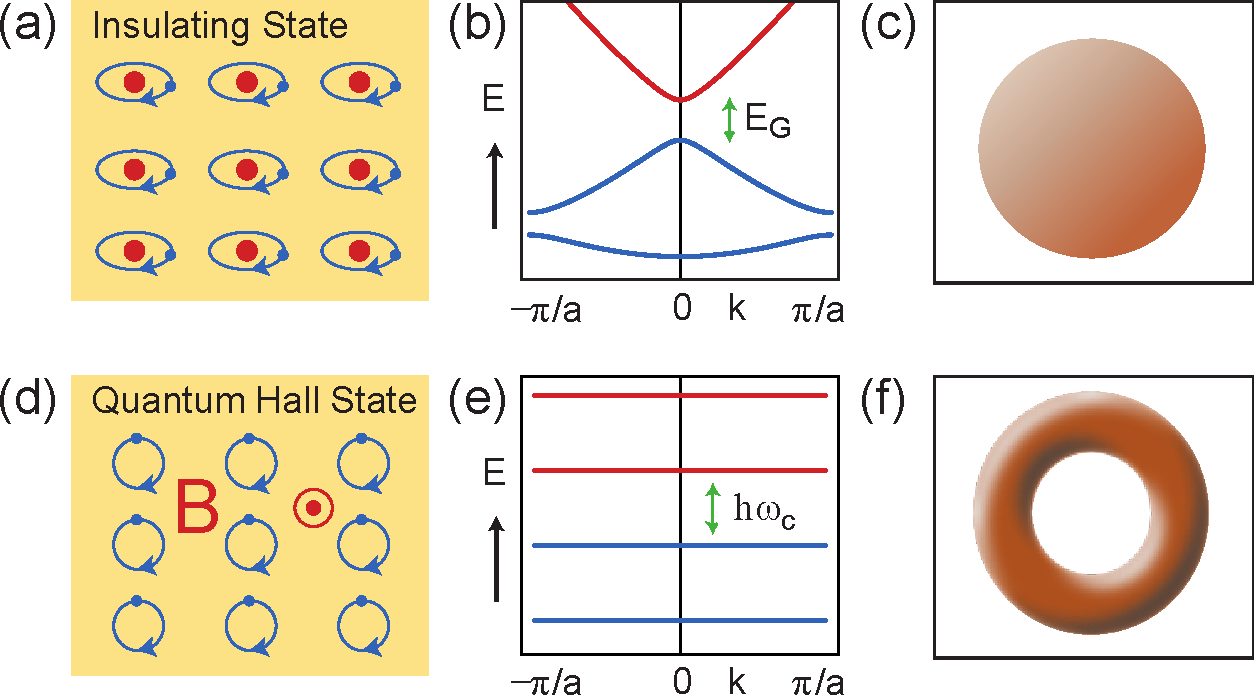
\includegraphics[width=3in]{Fig1}
		\caption{(a, b, c) The insulating state.  (a) depicts an atomic insulator, while
			(b) shows a simple model insulating band structure.  (d, e, f) The quantum Hall state.
			(d) depicts the cyclotron motion of electrons, and (e) shows the Landau levels, which may
			be viewed as a band structure.  (c) and (f) show two surfaces which differ in their genus, $g$.
			$g=0$ for the sphere (c) and $g=1$ for the donut (f).  The Chern number $n$ that distinguishes
			the two states is a topological invariant similar to the genus.}
		\label{fig:insulator}
	\end{figure}
	
	The simplest counterexample is the integer quantum Hall state
	\cite{vonklitzing80,prange87}, which
	occurs when electrons confined to two dimensions are placed in a
	strong magnetic field.  The quantization of the electrons' circular
	orbits with cyclotron frequency $\omega_c$
	leads to quantized Landau levels with
	energy $\epsilon_m=\hbar\omega_c (m+1/2)$.
	%, where $\omega_c$ is the cyclotron frequency.
	If $N$ Landau levels are filled and the rest are empty, then an energy gap
	separates the occupied and empty states just like in an
	insulator.  Unlike an insulator, though, an electric field causes
	the cyclotron orbits to drift, leading to a Hall
	current characterized by the quantized  Hall conductivity
	\begin{equation}
		\sigma_{xy} = N e^2/h.
		\label{qhall}
	\end{equation}
	The quantization of $\sigma_{xy}$ has been measured to
	one part in $10^9$ \cite{vonklitzing05}.  This precision is a
	manifestation of the topological nature of $\sigma_{xy}$.
	
	Landau levels can be viewed as a ``band
	structure".  Since the generators of translations do not commute with one another
	in a magnetic field, electronic states can
	not be labeled with momentum.  However, if a unit cell with
	area $2\pi \hbar c/e B$ enclosing a
	flux quantum is defined, then {\it lattice} translations
	{\it do} commute, so Bloch's theorem allows states to be labeled by
	2D crystal momentum ${\bf k}$.  In the absence of a periodic potential,
	the energy levels are simply the ${\bf k}$ independent
	Landau levels, $E_m({\bf k}) = \epsilon_m$.  In the presence of a periodic potential
	with the same lattice periodicity, the energy levels will
	disperse with ${\bf k}$.   This leads to a band structure
	%with a conduction band and a valence band separated by an energy gap
	that looks identical to that of an ordinary insulator.
	
	\subsubsection{The TKNN invariant}
	\label{sec:tknn}
	
	What is the difference between a
	quantum Hall state characterized by \eqref{qhall} and an ordinary insulator?
	The answer, explained in a seminal \citeyear{thouless82} paper by
	Thouless, Kohmoto, Nightingale and den Nijs(TKNN) is a matter of topology.
	A 2D band structure consists of a
	mapping from the crystal momentum ${\bf k}$ (defined on a torus)
	%$T^2$)
	to the Bloch Hamiltonian ${\cal H}({\bf k})$.
	%, a Hermitian matrix, with a set of eigenvalues $E_m({\bf k})$.
	Gapped band structures can
	be classified topologically by considering the equivalence classes of
	${\cal H}({\bf k})$ that can be continuously deformed into one another
	without closing the energy gap.  These classes are distinguished by a
	topological invariant $n \in \mathbb{Z}$ ($\mathbb{Z}$ denotes the integers)
	called the Chern invariant.
	
	The Chern invariant is rooted in the mathematical
	theory of fiber bundles\cite{nakahara90}, but it
	can be understood physically in terms of the Berry phase\cite{berry84} associated
	with Bloch wavefunctions $|u_m({\bf k})\rangle$.  Provided
	there are no accidental degeneracies, when ${\bf k}$ is transported around a
	closed loop, $|u_m({\bf k})\rangle$ acquires a well defined Berry phase given by the
	line integral of ${\cal A}_m = i\langle u_m|\nabla_k|u_m\rangle$.
	This may be expressed as a surface integral of the Berry
	flux, ${\cal F}_m = \nabla\times{\cal A}_m$.  The Chern invariant is the total
	Berry flux in the Brillouin zone,
	\begin{equation}
		n_m = \frac{1}{2\pi} \int d^2{\bf k} {\cal F}_m.
		\label{chern}
	\end{equation}
	$n_m$ is integer quantized for reasons analogous to the quantization of the
	Dirac magnetic monopole.  The total Chern number, summed over all occupied bands,
	$n = \sum_{m=1}^N n_m$
	is invariant even if there are degeneracies between
	occupied bands, provided the gap separating occupied and empty bands remains
	finite.
	TKNN showed that $\sigma_{xy}$, computed using the Kubo formula
	has the same form, so that $N$ in \eqref{qhall} is identical to
	$n$.  The Chern number $n$ is a topological
	invariant in the sense that it can not change when the Hamiltonian
	varies smoothly.   This helps
	to explain the robust quantization of $\sigma_{xy}$.
	
	%The topological classification of fiber bundles has been
	%known to mathematicians for 60 years \cite{nakahara90}.  Such bundles are classified by
	%the integers, $\mathbb{Z}$, and can be
	%distinguished by their first Chern class, given by
	%\begin{equation}
	%n = \frac{1}{2\pi} \int d^2{\bf k} {\cal F}
	% \label{chern}
	%\end{equation}
	%where the Berry's curvature ${\cal F} = \nabla\times{\cal A}$, and the
	%Berry's connection is ${\cal A} = i\sum_{m=1}^N \langle u_m|
	%\nabla_{\bf k}|u_m\rangle$.  \eqref{chern} can be interpreted as the
	%Berry's phase \cite{berry84} acquired by the valence band states when they are adiabatically
	%transported around the perimeter of the Brillouin zone.  It
	%has a structure similar to a winding number and is
	%guaranteed to be an integer.
	
	
	
	The meaning of \eqref{chern} can be clarified by a simple analogy.  Rather than
	maps from the Brillioun zone to a Hilbert
	space, consider simpler maps from 2D to 3D, which describe surfaces.  2D surfaces can be
	topologically classified by their genus, $g$, which counts the number of
	holes.  For instance, a sphere (Fig. \ref{fig:insulator}(c)) has $g=0$,
	while a donut (Fig. \ref{fig:insulator}(f)) has $g=1$.
	A beautiful theorem in mathematics due to Gauss and Bonnet \cite{nakahara90} states
	that the integral of the Gaussian
	curvature over a closed surface is a quantized topological invariant, and
	its value is related to $g$.  The Chern number is an integral
	of a related curvature.
	
	
	\subsubsection{Graphene, Dirac electrons, Haldane model}
	\label{sec:dirac}
	
	A simple example of the quantum Hall effect in a band theory
	is provided by a  model of graphene in a
	periodic magnetic field introduced by \textcite{haldane88}.  We will briefly digress
	here to introduce graphene because it will provide insight into the conception of the
	2D quantum spin Hall insulator, and because the physics of Dirac electrons
	present in graphene has important parallels at the surface of a 3D topological insulator.
	
	Graphene is a 2D form of carbon that is of high current interest
	\cite{novoselov05, zhangy05, geim07,neto09}.  What makes graphene interesting
	electronically is the fact that the conduction band and valence
	band touch each other at two distinct points in the Brillouin zone.  Near
	those points the electronic dispersion resembles the linear dispersion
	of massless relativistic particles, described by the Dirac equation
	\cite{divencenzo84,semenoff84}.
	The simplest description of graphene employs a two band model for
	the $p_z$ orbitals on the two equivalent atoms in the unit
	cell of graphene's honeycomb lattice.  The Bloch Hamiltonian is
	then a $2\times 2$ matrix,
	\begin{equation}
		{\cal H}({\bf k}) = {\bf h}({\bf k}) \cdot \vec \sigma,
		\label{dirac}
	\end{equation}
	where $\vec\sigma = (\sigma_x,\sigma_y,\sigma_z)$ are Pauli matrices
	and ${\bf h}({\bf k}) = (h_x({\bf k}),h_y({\bf k}),0)$.  The
	combination of inversion ($\cal P$) and time reversal ($\cal T$) symmetry requires
	$h_z({\bf k})=0$ because
	$\cal P$ takes $h_z({\bf k})$ to $-h_z(-{\bf k})$, while $\cal T$ takes
	$h_z({\bf k})$ to $+h_z(-{\bf k})$.  The Dirac points
	occur because the two component ${\bf h}({\bf k})$ can have point
	zeros in two dimensions.  In graphene they occur at two points,
	${\bf K}$ and ${\bf K}'=-{\bf K}$, whose locations at the
	Brillouin zone corners are fixed
	by graphene's rotational symmetry.  For small ${\bf q} \equiv {\bf k}-{\bf K}$,
	${\bf h}({\bf q}) = \hbar v_F {\bf q}$, where $v_F$ is a velocity,
	so ${\cal H}({\bf q}) = \hbar v_F {\bf q}\cdot\vec\sigma$
	has the form of a 2D massless Dirac Hamiltonian.
	
	The degeneracy at the Dirac point is protected by $\cal P$ and $\cal T$ symmetry.
	By breaking these symmetries the degeneracy
	can be lifted.  For instance, $\cal P$ symmetry is violated if the
	two atoms in the unit cell are inequivalent.  This allows
	$h_z({\bf k})$ to be non zero.  If $h_z({\bf k})$ is small, then
	near ${\bf K}$ \eqref{dirac} becomes a massive Dirac
	Hamiltonian,
	\begin{equation}
		{\cal H}({\bf q}) = \hbar v_F{\bf q}\cdot\vec\sigma + m \sigma_z
		\label{diracmass}
	\end{equation}
	where $m = h_z({\bf K})$.  The dispersion
	$E({\bf q}) = \pm \sqrt{|\hbar v_F {\bf q}|^2+m^2}$ has an
	energy gap $2|m|$ .  Note
	that ${\cal T}$ symmetry requires the Dirac point at ${\bf K}'$ has
	a mass $m'=h_z({\bf K}')$ with the same magnitude {\it and} sign, $m' = m$.  This state
	describes an ordinary insulator.
	
	\textcite{haldane88} imagined lifting the degeneracy by breaking ${\cal T}$
	symmetry with a magnetic field that is zero
	on the average, but has the full symmetry the lattice.  This
	perturbation allows nonzero $h_z({\bf k})$ and introduces a mass to
	the Dirac points.  However, $\cal P$ symmetry requires the masses at ${\bf
		K}$ and ${\bf K}'$
	have {\it opposite} sign, $m' = - m$. Haldane showed that this gapped
	state is not an insulator, but rather a quantum Hall state with
	%a quantized Hall conductivity
	$\sigma_{xy} = e^2/h$.
	
	This non-zero Hall conductivity can be understood in terms of
	\eqref{chern}.  For a two level Hamiltonian of the form of \eqref{dirac} it
	is well known that the Berry flux\cite{berry84} is related to
	the solid angle subtended by the unit vector $\hat h({\bf k}) =
	{\bf h}({\bf k})/|{\bf h}({\bf k})|$, so that \eqref{chern} takes the form
	\begin{equation}
		n = \frac{1}{4\pi}\int d^2{\bf k}
		(\partial_{k_x} \hat h \times \partial_{k_y} \hat h)\cdot \hat h .
	\end{equation}
	This simply counts the number of times $\hat h({\bf k})$ wraps around
	the unit sphere as a function of ${\bf k}$.  When the masses $m=m'=0$
	$\hat h({\bf k})$ is confined to the equator $h_z=0$, with a unit
	(and opposite)
	winding around each of the Dirac points where $|{\bf h}|=0$.
	For small but finite $m$, $|{\bf h}|\ne 0$ everywhere, and $\hat h({\bf K})$
	visits the north or south pole, depending on the sign of $m$.
	It follows that each Dirac point contributes $\pm e^2/2h$ to $\sigma_{xy}$.  In
	the insulating state with $m=m'$ the two cancel, so
	$\sigma_{xy}=0$. In the quantum Hall state they add.
	
	It is essential that there were an {\it even} number of Dirac points, since
	otherwise the Hall conductivity would be quantized to a half integer.  This is
	in fact guaranteed by the {\it fermion doubling theorem} \cite{nielssen83}, which states that for
	a ${\cal T}$ invariant system Dirac points must come in pairs.  We will
	return to this issue in section \ref{sec:3d}, where the surface of a topological
	insulator provides a loophole for this theorem.
	
	
	\subsubsection{Edge states and the bulk-boundary correspondence}
	\label{sec:edge}
	
	A fundamental consequence of the topological classification of gapped
	band structures is the existence of gapless conducting states at
	interfaces where the topological invariant changes.  Such edge states
	are well known at the interface between the integer quantum Hall
	state and vacuum \cite{halperin82}.  They may be understood in terms of the
	skipping motion electrons execute as their
	cyclotron orbits bounce off the edge (Fig. \ref{fig:qhalledge}(a)).
	Importantly, the electronic
	states responsible for this motion are {\it chiral} in the sense that
	they propagate in one direction only along the edge.  These states
	are insensitive to disorder because there are no states available for
	backscattering -- a fact that underlies the perfectly
	quantized electronic transport in the quantum Hall effect.
	
	The existence
	of such ``one way" edge states is deeply related to the topology of
	the bulk quantum Hall state.
	Imagine an interface where a crystal slowly interpolates as a
	function of distance $y$
	between a quantum Hall state ($n=1$) and a trivial insulator
	($n=0$).  Somewhere along the way the energy gap has to vanish,
	because otherwise it is impossible for the topological invariant to
	change.  There will therefore be low energy electronic states bound
	to the region where the energy gap passes through zero.  This interplay
	between topology and gapless modes is
	ubiquitous in physics, and has appeared in many contexts.
	It was originally found by \textcite{jackiw76} in their analysis of
	a 1D field theory.  Similar ideas were used by
	\textcite{su79} to describe soliton states in polyacetalene.
	
	A simple theory of the chiral edge states based on \textcite{jackiw76}
	can be developed using the
	two band Dirac model \eqref{diracmass}.  Consider an interface where
	the mass $m$ at one of the Dirac points changes sign as a function of $y$.
	We thus let $m \rightarrow m(y)$, where $m(y)>0$ gives the
	insulator for $y>0$ and $m(y)<0$ gives the quantum Hall state for $y<0$.
	Assume $m'>0$ is fixed.  The
	Schr\"odinger equation, obtained by replacing ${\bf q}$ by
	$-i \vec\nabla$ in \eqref{diracmass}, has a simple and elegant exact
	solution,
	\begin{equation}
		\psi_{q_x}(x,y) \propto e^{i q_x x} e^{-\int_0^y dy' m(y') dy'/v_F}
		\left(\begin{array}{c} 1\\1 \end{array}\right),
		\label{jackiwrebbi}
	\end{equation}
	with $E(q_x) = \hbar v_F q_x$.  This band of states intersects the
	Fermi energy $E_F$ with a positive group velocity $dE/dq_x = \hbar
	v_F$ and defines a right moving chiral edge mode.
	
	\begin{figure}
		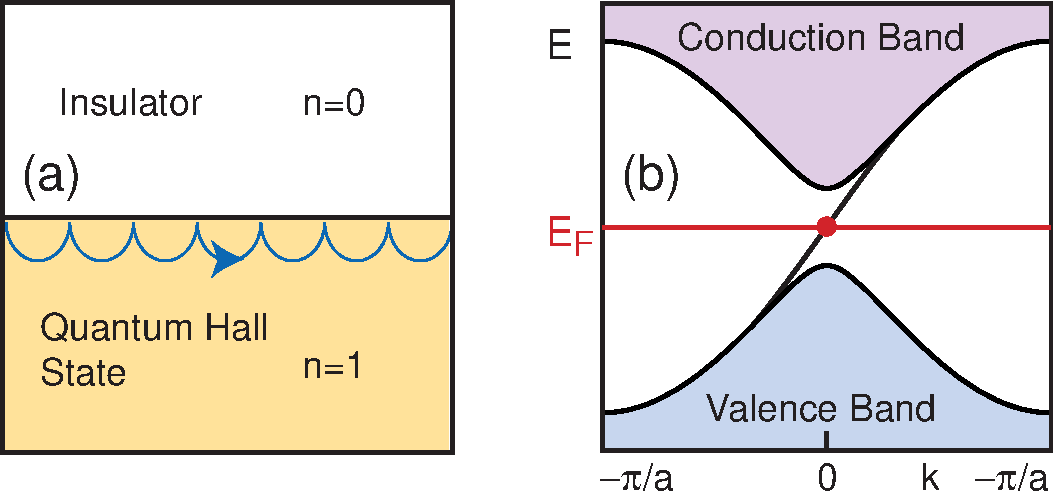
\includegraphics[width=3in]{Fig2}
		%\epsfxsize=3in
		%\epsfbox{Fig2.eps}
		\caption{The interface between a quantum Hall state and an insulator has chiral edge mode.
			(a) depicts the skipping cyclotron orbits.  (b) shows the electronic structure of a semi infinite
			strip described by the Haldane model.  A single edge state connects the valence band to the
			conduction band.}
		\label{fig:qhalledge}
	\end{figure}
	
	In the 1980's related ideas were applied to narrow gap
	semiconductors,
	which can be modeled using a 3D massive Dirac Hamiltonian\cite{volkov85,fradkin86}.
	An interface where the Dirac mass changes sign is associated with gapless 2D
	Dirac fermion states.  These share some similarities with
	the surface states of a 3D topological insulator, but as we shall see in
	section \ref{sec:strongweak}, there is a fundamental difference.
	In a separate development, \textcite{kaplan92} showed that in lattice
	quantum chromodynamics 4D chiral fermions could be simulated on
	a 5D lattice by introducing a similar domain wall.  This provided a method for circumventing the
	doubling theorem\cite{nielssen83}, which prevented the simulation of
	chiral fermions on a 4D lattice.  Quantum Hall edge states and surface states
	of a topological insulator evade similar doubling theorems.
	
	The chiral edge states in the quantum Hall effect can be seen explicitly by solving
	the Haldane model in a semi-infinite geometry with an edge at $y=0$.  Fig.
	\ref{fig:qhalledge}(b) shows the energy levels as a function of the momentum
	$k_x$ along the edge.  The solid regions show the bulk conduction and
	valence bands, which form continuum states and show the energy gap
	near ${\bf K}$ and ${\bf K}'$.  A single band, describing states
	bound to the edge connects the
	valence band to the conduction band with a positive group velocity.
	
	By changing the Hamiltonian near the surface the dispersion
	of the edge states can be modified.  For instance, $E(q_x)$ could
	develop a kink so that the edge states intersect $E_F$
	three times -- twice with a positive group velocity and once with a
	negative group velocity.  The difference $N_R-N_L$ between the number of right
	and left moving modes, however,
	can not change, and is determined by the topological structure of
	the bulk states.  This is summarized by the {\it bulk-boundary
		correspondence}:
	\begin{equation}
		N_R-N_L = \Delta n,
		\label{bulkboundary}
	\end{equation}
	where $\Delta n$ is the difference in the Chern number across the interface.
	
	
	
	\subsection{$Z_2$ topological insulator}
	\label{sec:z2topo}
	
	Since the Hall conductivity
	%(and hence the TKNN invariant)
	is odd under ${\cal T}$, the topologically non trivial
	states described in the preceding section
	can only occur when ${\cal T}$ symmetry is broken.
	However, the spin orbit interaction allows
	a {\it different} topological class of insulating band structures when ${\cal T}$
	symmetry is unbroken \cite{kanemele05a}.  The key to understanding this new
	topological class is to examine the role of ${\cal T}$ symmetry
	for spin 1/2 particles.
	
	${\cal T}$ symmetry is represented by an antiunitary operator
	$\Theta = \exp(i\pi S_y/\hbar) K$, where $S_y$ is the spin
	operator and $K$ is complex conjugation.
	For spin 1/2 electrons, $\Theta$ has the property $\Theta^2 = -1$.
	This leads to an important constraint, known as Kramers' theorem,
	that all eigenstates of a ${\cal T}$ invariant Hamiltonian
	%satisfying $[{\cal H},\Theta]=0$
	are at least twofold degenerate.
	This follows because if a non degenerate state $|\chi\rangle$ existed then
	$\Theta |\chi\rangle = c |\chi\rangle$ for some constant $c$.  This would mean $\Theta^2
	|\chi\rangle = |c|^2 |\chi\rangle$, which is not allowed because
	$|c|^2 \ne -1$.  In the absence of spin orbit interactions, Kramers'
	degeneracy is simply the degeneracy between up and down spins.  In
	the presence of spin orbit interactions, however, it has nontrivial
	consequences.
	
	A ${\cal T}$ invariant Bloch Hamiltonian must satisfy
	%${\cal T}$ symmetry imposes a constraint on the Bloch Hamiltonian,
	\begin{equation}
		\Theta {\cal H}({\bf k}) \Theta^{-1} = {\cal H}(-{\bf k}).
		\label{trsym}
	\end{equation}
	One can classify the equivalence classes of
	Hamiltonians satisfying this constraint that can be smoothly deformed
	without closing the energy gap.  The TKNN invariant is $n=0$, but
	there is an additional invariant with
	two possible values $\nu = 0$ or $1$ \cite{kanemele05b}.   The fact that there are two
	%and only two
	topological classes can be understood
	by appealing to the bulk-boundary correspondence.
	
	\begin{figure}
		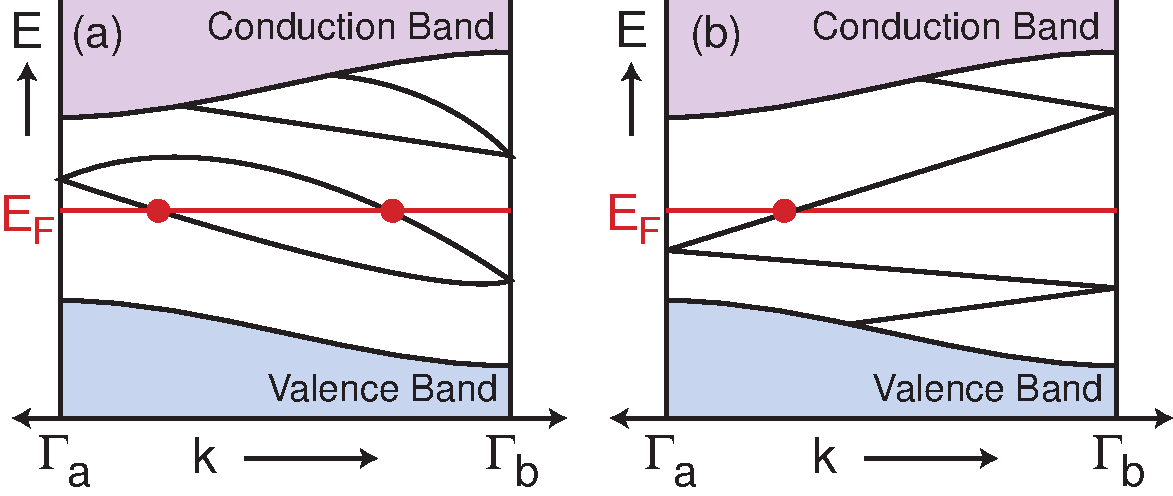
\includegraphics[width=3in]{Fig3}
		%\epsfxsize=3in
		%\epsfbox{Fig3.eps}
		\caption{Electronic dispersion between two boundary Kramers degenerate points
			$\Gamma_a=0$ and $\Gamma_b=\pi/a$.  In (a) the number of surface states crossing the Fermi
			energy $E_F$ is even, whereas in (b) it is odd.
			An odd number of crossings leads to topologically protected metallic boundary states.}
		\label{fig:zigzag}
	\end{figure}
	
	In Fig. \ref{fig:zigzag} we show plots analogous to Fig. \ref{fig:qhalledge} showing the electronic
	states associated with the edge of a ${\cal T}$ invariant 2D
	insulator as a function of the crystal momentum along the edge.  Only
	half of the Brillouin zone $0<k_x<\pi/a$ is shown because ${\cal T}$
	symmetry requires that the other
	half $-\pi/a<k<0$ is a mirror image.  As in Fig. \ref{fig:qhalledge}, the
	shaded regions depict the bulk conduction and valence bands separated by an
	energy gap.  Depending on the details of the Hamiltonian near the
	edge there may or may not be states bound to the edge inside the gap.
	If they are present, however, then Kramers
	theorem requires they be twofold degenerate at the ${\cal T}$
	invariant momenta $k_x=0$ and $k_x=\pi/a$ (which is the same as
	$-\pi/a$). Away from these special points, labeled $\Gamma_{a,b}$ in
	Fig. \ref{fig:zigzag}, a spin orbit
	interaction will split the degeneracy.  There are two
	ways the states at $k_x=0$ and $k_x=\pi/a$ can connect.  In
	Fig \ref{fig:zigzag}(a) they connect pairwise.  In this case
	the edge states can be eliminated by pushing all of the bound
	states out of the gap. Between $k_x=0$ and $k_x=\pi/a$, the bands intersect
	$E_F$ an even number of times. In contrast, in Fig. \ref{fig:zigzag}b the
	edge states cannot be eliminated.  The bands intersect $E_F$
	an odd number of times.
	
	Which of these alternatives occurs depends on
	the topological class of the bulk band structure.  Since each band intersecting
	$E_F$ at $k_x$ has a Kramers partner at $-k_x$, the bulk-boundary
	correspondence relates the number $N_K$ of Kramers pairs of edge
	modes intersecting $E_F$ to the change in the $\mathbb{Z}_2$
	invariants across the interface,
	\begin{equation}
		N_K = \Delta \nu \ {\rm mod} \ 2.
	\end{equation}
	We conclude that a 2D topological insulator has
	topologically protected edge states.  These form a unique
	1D conductor, whose properties will be discussed in section
	\ref{sec:qshi}.  The above considerations can be generalized to
	3D topological insulators, discussed in section \ref{sec:3d},
	which have protected surface states.
	
	There are several mathematical formulations of the $\mathbb{Z}_2$ invariant $\nu$
	\cite{kanemele05b,fukane06,moorebalents07,fukane07,fukui07,fukui08,qihugheszhang08,roy09a,wang09}.  One
	approach \cite{fukane06} is to define a unitary matrix
	$w_{mn}({\bf k}) = \langle u_m({\bf k})|\Theta|u_n(-{\bf k})\rangle$
	built from the occupied Bloch functions
	$|u_m({\bf k})\rangle$.  Since $\Theta$ is anti unitary
	and $\Theta^2=-1$, $w^T({\bf k}) = - w(-{\bf k})$.  There are four
	special points $\Lambda_a$ in the bulk 2D Brillouin zone where ${\bf k}$ and
	$-{\bf k}$ coincide, so $w(\Lambda_a)$ is
	antisymmetric.  The determinant of an antisymmetric matrix is the square of
	its pfaffian, which allows us to define
	$\delta_a = {\rm Pf}[w(\Lambda_a)]/\sqrt{{\rm Det}[w(\Lambda_a)]} = \pm 1$.
	{\it Provided} $|u_m({\bf k})\rangle$ is chosen continuously
	throughout the Brillouin zone (which is always possible), the branch
	of the square root can be specified globally, and the $\mathbb{Z}_2$
	invariant is
	\begin{equation}
		(-1)^\nu = \prod_{a=1}^4 \delta_a.
		\label{deltaa}
	\end{equation}
	This formulation can be
	generalized to 3D topological insulators, and involves
	the 8 special points in the 3D Brillouin zone.
	
	The calculation of $\nu$ is simpler
	if the crystal has extra symmetry.  For instance, if the 2D system
	conserves the perpendicular spin $S_z$, then the
	up and down spins have independent
	Chern integers $n_\uparrow$, $n_\downarrow$.
	${\cal T}$ symmetry requires $n_\uparrow+n_\downarrow = 0$, but
	the difference $n_\sigma = (n_\uparrow-n_\downarrow)/2$ defines a quantized spin
	Hall conductivity \cite{sheng06}.  The $\mathbb{Z}_2$ invariant is then simply
	\begin{equation}
		\nu = n_\sigma \ {\rm mod} \ 2.
	\end{equation}
	While $n_\uparrow$, $n_\downarrow$ lose
	their meaning when $S_z$ non conserving terms (which
	are inevitably present) are added, $\nu$ retains its identity.
	
	If the crystal has inversion symmetry there is another shortcut to
	computing $\nu$ \cite{fukane07}.  At the special points $\Lambda_a$
	the Bloch states $u_m(\Lambda_a)$ are also parity eigenstates with eigenvalue
	$\xi_m(\Lambda_a)=\pm 1$.  The $\mathbb{Z}_2$ invariant then simply
	follows from \eqref{deltaa} with
	\begin{equation}
		\delta_a = \prod_{m} \xi_m(\Lambda_a),
		\label{parityz2}
	\end{equation}
	where the product is over the Kramers pairs of occupied bands.
	This has proven useful for identifying
	topological insulators from band structure calculations
	\cite{fukane07,teofukane08,zhangh09,pesin10,guo09}.
	
	
	\subsection{Topological superconductor, Majorana fermions}
	\label{sec:superconductor}
	
	Considerations of topological band theory can also be used to
	topologically classify superconductors.  This is a subject that has seen
	fascinating recent theoretical
	developments \cite{schnyder08,kitaev09,qihughesraduzhang09,roy08}.
	%Space precludes a
	%detailed description of topological superconductors.
	We will give an introduction that focuses on the simplest
	model superconductors.  The more
	general case will be briefly touched on at the end.  This section will provide
	the conceptual basis for topological superconductors and explain
	the emergence of Majorana fermions in superconducting
	systems.  It will also provide background for section \ref{sec:proximity}, where we
	discuss Majorana states in superconductor-topological
	insulator structures along with possible applications to topological
	quantum computing.  Readers who wish to skip the discussion of superconductivity
	can proceed directly to section \ref{sec:qshi}.
	
	\subsubsection{Bogoliubov de Gennes theory}
	\label{sec:bdg}
	
	In the BCS mean field theory of a superconductor the Hamiltonian for a system
	of spinless electrons may be written in the form \cite{degennes66},
	\begin{equation}
		H-\mu N =
		\frac{1}{2}\sum_{\bf k} \left(\begin{array}{cc} c_{\bf k}^\dagger & c_{-{\bf k}} \end{array}\right)
		{\cal H}_{BdG}({\bf k})
		\left(\begin{array}{c} c_{\bf k} \\ c_{-{\bf k}}^\dagger \end{array}\right)
		\label{bdg}
	\end{equation}
	where $c_{\bf k}^\dagger$ is an electron creation operator and
	${\cal H}_{BdG}$ is a $2 \times 2$ block matrix, which in Nambu's notation
	may be written in terms of Pauli matrices $\vec\tau$ as
	\begin{equation}
		{\cal H}_{BdG}({\bf k}) = ({\cal H}_0({\bf k})-\mu) \tau_z + \Delta_1({\bf k})
		\tau_x + \Delta_2({\bf k}) \tau_y.
	\end{equation}
	Here ${\cal H}_0({\bf k})$ is the Bloch Hamiltonian in the absence of
	superconductivity and $\Delta = \Delta_1 + i\Delta_2$ is the BCS mean
	field pairing potential, which for spinless particles must have odd parity,
	$\Delta(-{\bf k}) = -\Delta({\bf k})$.
	For a uniform system the excitation spectrum
	of a superconductor is given by the eigenvalues of ${\cal
		H}_{BdG}$, which exhibit a superconducting energy gap.  More generally, for
	spatially dependent ${\cal H}_0$ and
	$\Delta$ the Schr\"odinger equation associated with ${\cal H}_{BdG}$ is
	known as the Bogoliubov de Gennes (BdG) equation.
	
	Since \eqref{bdg} has both $c$ and $c^\dagger$ on both sides there is
	an inherent redundancy built into the BdG Hamiltonian.  For
	$\Delta=0$, ${\cal H}_{BdG}$ includes
	two copies of ${\cal H}_0$ with opposite sign.  More generally, ${\cal H}_{BdG}$
	has an intrinsic {\it particle-hole symmetry} expressed by
	\begin{equation}
		\Xi {\cal H}_{BdG}({\bf k}) \Xi^{-1} = - {\cal H}_{BdG}(-{\bf k}),
		\label{phsym}
	\end{equation}
	where the particle-hole operator, $\Xi = \tau_x K$,
	satisfies $\Xi^2 = +1$.  \eqref{phsym} follows from ${\cal H}_0(-{\bf k})={\cal H}_0({\bf k})^*$
	and the odd parity of the real $\Delta({\bf k})$.  It follows that every
	eigenstate of ${\cal H}_{BdG}$ with energy $E$ has a partner at
	$-E$.  These two states are redundant because the
	Bogoliubov quasiparticle operators associated with them satisfy
	$\Gamma_E^\dagger = \Gamma_{-E}$.  Thus, creating a quasiparticle in state
	$E$ has the same effect as removing one from state $-E$.
	
	The particle-hole symmetry constraint \eqref{phsym} has a similar
	structure to the time reversal constraint in \eqref{trsym}, so it is
	natural to consider the classes of BdG Hamiltonians that
	can be continuously deformed into one another without closing the
	energy gap.  In the simplest case, spinless fermions, the classification
	can be shown to be $\mathbb{Z}_2$
	in one dimension and $\mathbb{Z}$ in two dimensions.
	As in section \ref{sec:z2topo}, this can be most easily understood by appealing to
	the bulk-boundary correspondence.
	
	\subsubsection{Majorana fermion boundary states}
	\label{sec:majoranaedge}
	
	At the end of a 1D superconductor \cite{kitaev00} there may or may not
	be discrete states within the energy gap that are bound to the end
	(Fig. \ref{fig:scedge}(a-c)).
	If they are present, then every state at $+E$ has a partner at
	$-E$.  Such finite energy pairs are not topologically protected
	because they can simply be pushed out of the energy gap.  However,
	a single {\it unpaired} bound state at $E=0$ {\it is} protected because it can't move away
	from $E=0$.  The presence or absence of such a zero mode is determined by the
	$\mathbb{Z}_2$ topological class of the bulk 1D superconductor.
	
	\begin{figure}
		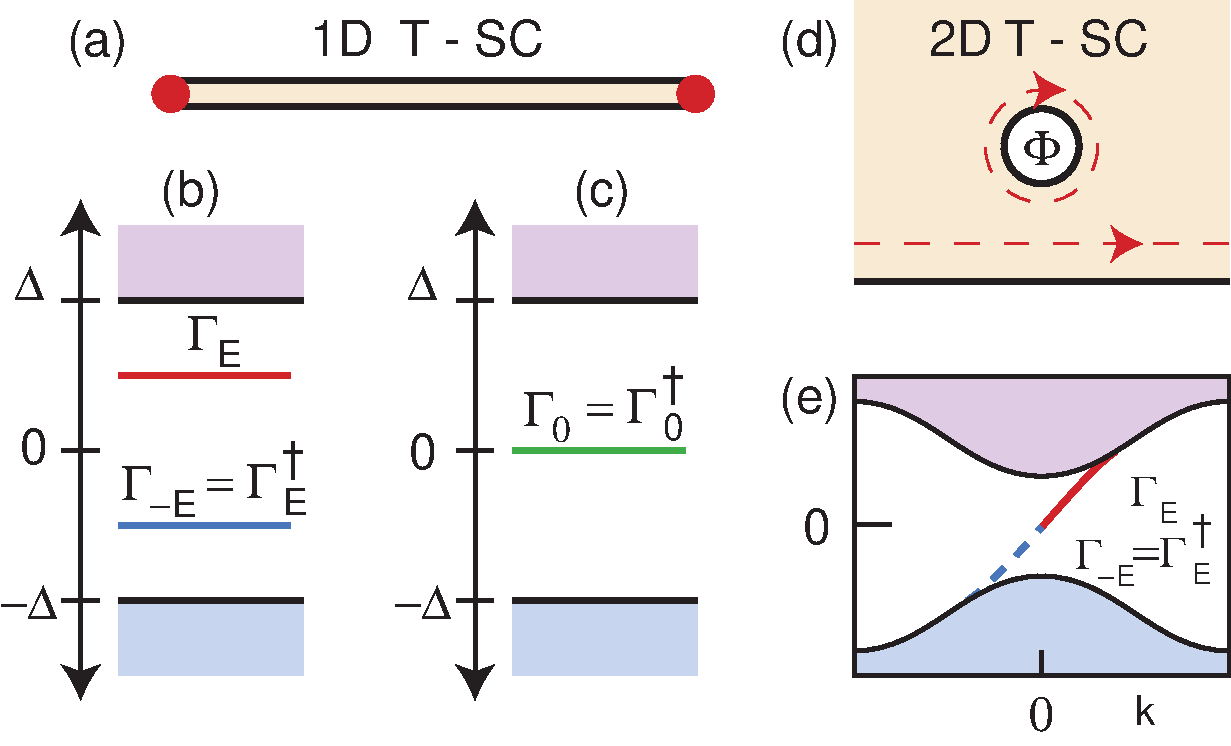
\includegraphics[width=3in]{Fig4}
		%\epsfxsize=3in
		%\epsfbox{Fig4.eps}
		\caption{Boundary states for a topological superconductor (T-SC).  (a) shows a 1D superconductor
			with bound states at its ends.  (b,c) show the end state spectrum for an ordinary 1D superconductor
			(b) and a 1D topological superconductor (c).  (d) shows a topological 2D superconductor
			with a chiral Majorana edge mode (e).  A vortex with flux $\Phi = h/2e$ is associated
			with a zero mode (c).}
		\label{fig:scedge}
	\end{figure}
	
	The Bogoliubov quasiparticle states associated with the zero modes are
	fascinating objects \cite{nayak08,readgreen00,stern04,ivanov01,kitaev00}.  Due to the particle-hole redundancy
	the quasiparticle operators satisfy $\Gamma_0 = \Gamma_0^\dagger$.
	Thus, a quasiparticle is its own antiparticle -- the defining
	feature of a {\it Majorana fermion}.
	A Majorana fermion is essentially {\it half} of an ordinary
	Dirac fermion.  Due to the particle-hole redundancy, a single fermionic state
	is associated with each {\it pair} of $\pm E$ energy levels.  The presence or absence
	of a fermion in this state defines a two level system with energy splitting $E$.
	Majorana zero modes
	must always come in pairs (for instance, a 1D superconductor has two ends), and a
	well separated pair
	defines a {\it degenerate} two level system, whose quantum state is stored nonlocally.
	This has profound implications, which we will return to in section
	\ref{sec:proximity}, when we discuss the proposal by \textcite{kitaev03} to use these
	properties for quantum information processing.
	
	In two dimensions the integer classification, $\mathbb{Z}$,
	gives the number of {\it chiral Majorana} edge
	modes (Fig. \ref{fig:scedge}(d,e)), which resemble chiral modes in the quantum Hall effect, but for
	the particle-hole redundancy.  A spinless superconductor with $p_x+ip_y$ symmetry
	is the simplest model 2D topological superconductor.
	Such superconductors will also exhibit Majorana bound states at the core of vortices
	\cite{caroli64,volovik99,readgreen00}.
	This may be understood simply by considering the vortex to be a hole
	in the superconductor circled by an edge mode (Fig. \ref{fig:scedge}(d)).
	When the flux in the
	hole is $h/2e$ the edge modes are quantized such that one state is exactly
	at $E=0$.
	
	Majorana fermions have been studied in particle
	physics for decades, but have not been definitively observed \cite{majorana37,wilczek09}.
	A neutrino {\it might} be a Majorana fermion.  Efforts to observe
	certain lepton number violating
	neutrinoless double $\beta$ decay processes may resolve that issue \cite{avignone08}.
	In condensed matter physics, Majorana fermions can arise due to
	a paired condensate that allows a pair of fermionic quasiparticles to
	``disappear" into the condensate.  They have been predicted in a
	number of physical systems related to the spinless
	$p_x+i p_y$ superconductor, including the Moore-Read state of the
	$\nu=5/2$ quantum Hall effect \cite{mooreread91,greiter92,readgreen00}, Sr$_2$RuO$_4$ \cite{dassarma06},
	cold fermionic atoms near a Feshbach resonance \cite{gurarie05,tewari07} and
	2D structures that combine superconductivity, magnetism and strong
	spin orbit coupling \cite{sato09,sau10,lee09}.
	In Section Vb we will discuss the prospect for creating
	Majorana fermion states at interfaces between topological
	insulators and ordinary superconductors \cite{fukane08}.
	
	\subsubsection{Periodic table}
	\label{sec:periodic}
	
	Topological insulators and superconductors fit together into a rich and elegant
	mathematical structure that generalizes the notions of topological band
	theory described above \cite{schnyder08,schnyder09,kitaev09,ryu09}.  The classes of equivalent Hamiltonians are determined by specifying the
	symmetry class and the dimensionality.  The symmetry class depends on
	the presence or absence of ${\cal T}$ symmetry \eqref{trsym} with $\Theta^2=\pm 1$ and/or
	particle-hole symmetry \eqref{phsym} with $\Xi^2=\pm 1$.  There are 10 distinct classes,
	which are closely related to the \textcite{altland97} classification of random
	matrices.  The topological classifications, given by
	$\mathbb{Z}$, $\mathbb{Z}_2$ or $0$, show a regular pattern as a function of
	symmetry class and dimensionality and can be arranged into the {\it periodic
		table} of topological insulators and superconductors shown in Table \ref{tab:periodic}.
	
	\begin{table}
		\centering
		\begin{ruledtabular}
			\begin{tabular}{c|ccc|cccccccc}
				\multicolumn{4}{c|}{Symmetry } & \multicolumn{8}{c}{ $d$} \\
				% after \\ : \hline or \cline{col1-col2} \cline{col3-col4} ...
				\multicolumn{1}{c}{AZ} &$\hspace{1.5mm}\Theta\hspace{1.5mm} $ &
				$\hspace{1.5mm} \Xi\hspace{1.5mm} $ &
				$\hspace{1.5mm} \Pi\hspace{1.5mm} $ &
				$1$   &  $2$ &  $3$ &  $4$ &  $5$ & $6$ & $7$& $8$ \\
				\hline
				A & $0$ & $0$ & $0$  &$0$& $\mathbb{Z}$ &$0$& $\mathbb{Z}$ &$0$& $\mathbb{Z}$ &$0$& $\mathbb{Z}$\\
				AIII & $0$ & $0$ & $1$ & $\mathbb{Z}$ &$0$& $\mathbb{Z}$ &$0$& $\mathbb{Z}$ &$0$& $\mathbb{Z}$& $0$\\
				\hline
				AI & $1$ & $0$ & $0$  &$0$&$0$&$0$&$\mathbb{Z}$&$0$&$\mathbb{Z}_2$&$\mathbb{Z}_2$& $\mathbb{Z}$ \\
				BDI & $1$ &$1$ &$1$ & $\mathbb{Z}$ &$0$&$0$&$0$&$\mathbb{Z}$&$0$&$\mathbb{Z}_2$& $\mathbb{Z}_2$\\
				D & $0$ &$1$ &$0$ & $\mathbb{Z}_2$& $\mathbb{Z}$ &$0$&$0$&$0$&$\mathbb{Z}$&$0$&$\mathbb{Z}_2$\\
				DIII&$-1$ &$1$ &$1$ &$\mathbb{Z}_2$& $\mathbb{Z}_2$& $\mathbb{Z}$ &$0$&$0$&$0$&$\mathbb{Z}$&$0$\\
				AII & $-1$ & $0$ & $0$ &$0$&$\mathbb{Z}_2$& $\mathbb{Z}_2$& $\mathbb{Z}$ &$0$&$0$& $0$&$\mathbb{Z}$\\
				CII & $-1$ &$-1$ & $1$&$\mathbb{Z}$ & $0$&$\mathbb{Z}_2$& $\mathbb{Z}_2$& $\mathbb{Z}$ &$0$&$0$&$0$ \\
				C & $0$ & $-1$& $0$ & $0$ &$\mathbb{Z}$ &$0$&$\mathbb{Z}_2$& $\mathbb{Z}_2$& $\mathbb{Z}$ &$0$& $0$\\
				CI & $1$ & $-1$ & $1$& $0$ & $0$&$\mathbb{Z}$&$0$&$\mathbb{Z}_2$& $\mathbb{Z}_2$& $\mathbb{Z}$& $0$ \\
				
			\end{tabular}
		\end{ruledtabular}
		\caption{Periodic table of topological insulators and superconductors.  The 10 symmetry
			classes are labeled using the notation of \textcite{altland97} (AZ) and are
			specified by presence or absence of ${\cal T}$ symmetry
			$\Theta$, particle-hole symmetry $\Xi$ and chiral symmetry $\Pi = \Xi\Theta$.
			$\pm 1$ and $0$ denotes the presence and absence of symmetry,
			with $\pm 1$ specifying the value of $\Theta^2$ and
			$\Xi^2$.  As a function of symmetry and space dimensionality, $d$, the topological
			classifications ($\mathbb{Z}$, $\mathbb{Z}_2$ and $0$) show a regular pattern
			that repeats when $d \rightarrow d+8$.  }
		\label{tab:periodic}
	\end{table}
	
	
	
	The quantum Hall state (Class A, no symmetry; $d=2$), the $\mathbb{Z}_2$ topological
	insulators (Class AII, $\Theta^2=-1$; $d=2,3$) and the $\mathbb{Z}_2$ and $\mathbb{Z}$ topological
	superconductors (Class D, $\Xi^2=1$; $d=1,2$) described above are each entries in the periodic table.
	There are also other non trivial entries describing different topological
	superconducting and superfluid phases.  Each non trivial phase is predicted,
	via the bulk-boundary correspondence to have gapless boundary states.  One
	notable example is superfluid $^3$He B \cite{schnyder08,roy08,nagato09,qihughesraduzhang09,volovik03,volovik09}, in
	(Class DIII, $\Theta^2=-1$, $\Xi^2=+1$; $d=3$) which has a $\mathbb{Z}$
	classification, along with gapless 2D Majorana fermion modes on its
	surface.   A generalization of the quantum Hall state introduced by
	\textcite{zhang01} corresponds to the $d=4$ entry in class A or AII.
	There are also other entries
	%in the table
	in physical dimensions that have yet to
	be filled by realistic systems.  The search is on to discover such
	phases.
	
	
	\section{Quantum Spin Hall Insulator}
	\label{sec:qshi}
	
	The 2D topological insulator is known as a quantum spin
	Hall insulator.  This state was originally theorized to exist in
	graphene \cite{kanemele05a} and in 2D semiconductor systems with a uniform
	strain gradient \cite{bernevig06}.  It was subsequently predicted to exist \cite{bernevighugheszhang06}, and was
	then observed \cite{konig07}, in HgCdTe quantum well structures.  In section \ref{sec:graphene} we
	will introduce the physics of this state in the model graphene system
	and describe its novel edge states.  Section \ref{sec:hgcdte} will
	review the experiments, which have also been the subject of the review article
	by \textcite{konig08}.
	
	\subsection{Model system: graphene}
	\label{sec:graphene}
	
	\begin{figure}
		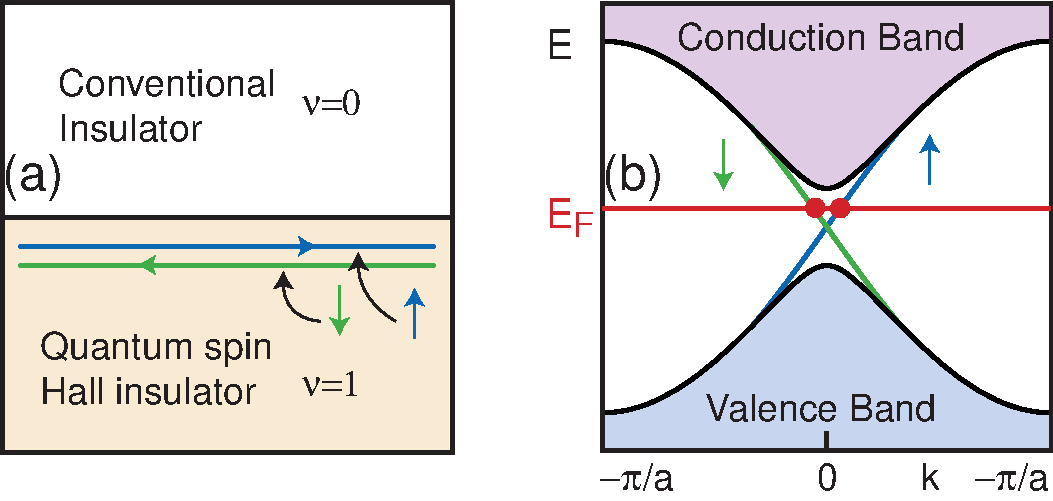
\includegraphics[width=3in]{Fig5}
		%\epsfxsize=3in
		%\epsfbox{Fig5.eps}
		\caption{Edge states in the quantum spin Hall insulator.  (a) shows the interface between a
			QSHI and an ordinary insulator, and (b) shows the edge state dispersion in the graphene model,
			in which up and down spins propagate in opposite directions.}
		\label{fig:qshedge}
	\end{figure}
	
	In section \ref{sec:dirac} we argued that the degeneracy at the Dirac
	point in graphene is protected by inversion and ${\cal T}$
	symmetry.  That argument ignored the spin of the
	electrons.  The spin orbit interaction allows a new mass
	term in \eqref{dirac} that respects {\it all} of graphene's
	symmetries.
	In the simplest picture, the intrinsic spin orbit interaction
	commutes with the electron spin $S_z$, so the Hamiltonian decouples
	into two independent Hamiltonians for the up and down spins.  The
	resulting theory is simply two copies the \textcite{haldane88} model
	with opposite signs of the Hall conductivity for up and down spins.
	This does not violate ${\cal T}$ symmetry because time reversal
	flips both the spin and $\sigma_{xy}$.  In an applied
	electric field, the up and down spins have Hall currents that flow in
	opposite directions.  The Hall conductivity is thus zero, but there
	is a quantized {\it spin Hall} conductivity, defined by
	$J_x^\uparrow-J_x^\downarrow = \sigma_{xy}^s E_y$ with
	$\sigma_{xy}^s = e/2\pi$ --
	a quantum spin Hall effect.  Related ideas were mentioned in
	earlier work on the planar state of $^3$He films\cite{volovik89}.
	Since it is two copies a quantum Hall state, the quantum
	spin Hall state must have gapless edge states (Fig. \ref{fig:qshedge}).
	
	The above discussion was predicated on the conservation of
	spin, $S_z$.  This is not a fundamental symmetry, though, and spin
	non conserving processes -- present in any real system -- invalidate the
	meaning of $\sigma_{xy}^s$.  This brings into
	question theories that relied on spin conservation to predict an
	integer quantized $\sigma_{xy}^s$ \cite{volovik89,bernevig06,qi06}, as well as the
	influential theory of the (non quantized) spin Hall insulator \cite{murakami04}.
	\textcite{kanemele05a} showed that due to ${\cal T}$ symmetry
	the edge states in the quantum spin Hall insulator are robust
	even when spin conservation is violated because their crossing at $k=0$ is
	protected by the Kramers degeneracy discussed in section
	\ref{sec:z2topo}.  This established the quantum spin Hall insulator as a
	topological phase.
	
	The quantum spin Hall edge states have the
	important ``spin filtered" property that the up spins propagate in one direction,
	while the down spins propagate in the other.  Such edge states were later dubbed
	``helical" \cite{wu06}, in analogy with the correlation between spin and momentum
	of a particle known as helicity.
	They form a unique 1D conductor that is essentially {\it half} of an ordinary 1D conductor.
	Ordinary conductors, which have both up and down spins propagating in
	both directions, are fragile because the electronic states are
	susceptible to Anderson localization in the presence of weak
	disorder \cite{anderson58,lee85}.  By contrast, the quantum spin Hall edge states can not be localized,
	even for strong disorder.  To see this, imagine an edge that is
	disordered in a finite region, and perfectly clean outside that
	region.  The exact eigenstates can be determined by solving the
	scattering problem relating incoming waves to those reflected from
	and transmitted through the disordered region.  \textcite{kanemele05a}
	showed that the reflection amplitude is {\it odd} under ${\cal T}$
	-- roughly because it involves flipping the spin.  It
	follows that unless ${\cal T}$ symmetry is broken, an incident
	electron is transmitted {\it perfectly} across the disordered region.
	Thus, eigenstates at any energy are extended, and
	at temperature $T=0$, the edge state transport is
	ballistic.  For $T>0$ inelastic backscattering processes are
	allowed, which will in general lead to a finite conductivity.
	
	The edge states are similarly protected from the
	effects of weak electron interactions, though for strong interactions Luttinger liquid
	effects lead to a magnetic instability \cite{wu06,xu06}.   This
	strongly interacting phase is interesting because it will
	exhibit charge $e/2$ quasiparticles similar to
	solitons in the \textcite{su79} model.  For sufficiently strong interactions
	similar fractionalization could
	be observed by measuring shot noise in the presence of magnetic
	impurities \cite{maciejko09} or at a quantum point contact \cite{teokane09}.
	
	\subsection{HgTe/CdTe quantum well structures}
	\label{sec:hgcdte}
	
	Graphene is made out of carbon -- a
	light element with a weak spin orbit interaction.  Though there
	is disagreement on its absolute magnitude \cite{min06,huertas06,yao07,boettger07,gmitra09},
	the energy gap in graphene is likely to be small.
	Clearly, a better place to look for this physics would be in
	materials with strong spin orbit interactions, made from
	heavy elements near the bottom of the periodic table.
	To this end, \textcite{bernevighugheszhang06} (BHZ) had the brilliant idea to
	consider quantum well structures of HgCdTe.  This paved
	the way to the experimental discovery of the quantum spin Hall
	insulator phase.
	
	%\subsubsection{Band inversion transition}
	%\label{sec:inversion}
	
	Hg$_{1-x}$Cd$_x$Te is a family of semiconductors with strong spin orbit
	interactions \cite{dornhaus83}.  CdTe has a band structure similar to other
	semiconductors.  The conduction band edge states have an $s$ like symmetry,
	while the valence band edge states have a $p$ like symmetry.
	In HgTe, the $p$ levels rise above the $s$ levels, leading to an {\it inverted}
	band structure.  BHZ considered a quantum well structure where HgTe is
	sandwiched between layers of CdTe.  When the thickness of the HgTe layer is
	$d < d_c= 6.3$ nm the 2D electronic states bound to the quantum well have the
	normal band order.  For $d > d_c$, however, the 2D bands
	invert.  BHZ showed that the inversion of the bands as a function of increasing $d$ signals a
	quantum phase transition between the trivial insulator and the quantum spin
	Hall insulator.   This can be understood simply in the approximation that
	the system has inversion symmetry.  In this case, since the $s$ states
	and $p$ states have opposite parity the bands will cross each other at $d_c$ without
	an avoided crossing.  Thus the energy gap at $d=d_c$ vanishes.
	From \eqref{parityz2}, the change in the parity of
	the valence band-edge state signals a phase transition in which
	the $\mathbb{Z}_2$ invariant $\nu$ changes.
	
	\begin{figure}
		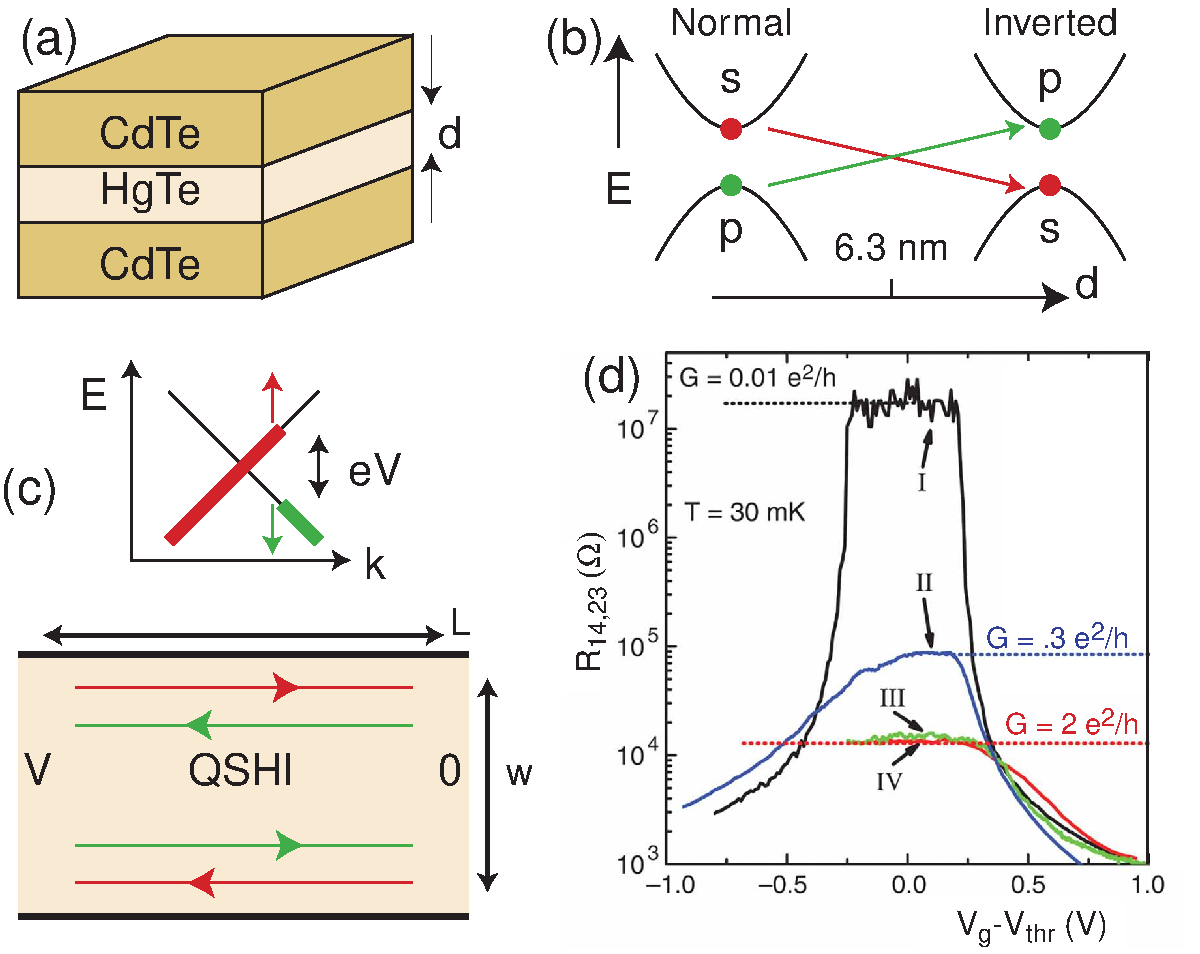
\includegraphics[width=3in]{Fig6}
		%\epsfxsize=3in
		%\epsfbox{Fig6.eps}
		%\epsfbox{mk.eps}
		\caption{(a) A HgCdTe quantum well structure.  (b) As a function of layer thickness
			$d$ the 2D quantum well states cross at a band inversion transition.  The
			inverted state is the QSHI, which has helical edge states (c) that
			have a non equilibrium population determined by the leads.  (d) shows
			experimental two terminal conductance as a function of a gate voltage that
			tunes $E_F$ through the bulk gap.    Sample I, with $d<d_c$ shows insulating
			behavior, while samples III and IV show quantized transport associated with
			edge states.  Adapted from \onlinecite{konig07}.  Reprinted with permission from AAAS.}
		\label{fig:hgcdtefig}
	\end{figure}
	
	%\subsubsection{Transport experiments}
	%\label{sec:transport}
	
	Within a year of the theoretical proposal the W\"urzburg group, led by Laurens
	Molenkamp, made the devices and performed transport experiments that
	showed the first signature of the quantum spin Hall insulator.
	\textcite{konig07}
	measured the electrical conductance due to the edge states.
	The low temperature ballistic edge state transport
	can be understood within a simple Landauer-B\"uttiker
	\cite{buttiker88}
	framework in which the edge states are populated according to the
	chemical potential of the lead that they emanate from.  This leads to
	a quantized conductance $e^2/h$ associated with each set of edge
	states.  Fig. \ref{fig:hgcdtefig}(d) shows the resistance measurements for a series of
	samples as a function of a gate voltage which tunes the Fermi energy
	through the bulk energy gap.  Sample I is a narrow quantum well
	that has a large resistance in the gap.  Samples II, III and IV are
	wider wells in the inverted regime.   Samples III and IV exhibit a
	conductance $2e^2/h$ associated with the top and bottom edges.  Samples III and IV have
	the same length $L = 1\mu$ but different widths
	$w = 0.5\mu,1\mu$, indicating transport is at the edge.  Sample
	II  ($L=20\mu$) showed finite temperature scattering effects. These
	experiments convincingly demonstrate the existence of the edge
	states of the quantum spin Hall insulator.  Subsequent
	experiments have established the inherently nonlocal electronic
	transport in the edge states \cite{roth09}.
	
	
	\section{3D Topological Insulators}
	\label{sec:3d}
	
	In the summer of 2006 three groups of theorists independently discovered that the
	topological characterization of the quantum spin Hall insulator state
	has a natural generalization in three dimensions \cite{fukanemele07,moorebalents07,roy09b}.
	\textcite{moorebalents07} coined the term ``topological
	insulator" to describe this electronic phase.  \textcite{fukanemele07} established the
	connection between the bulk topological order and the presence of unique conducting surface
	states.  Soon after, this phase was predicted in several real materials \cite{fukane07}, including
	Bi$_{1-x}$Sb$_x$ as well as strained HgTe and $\alpha-$Sn.  In 2008, \textcite{hsieh08}
	reported the experimental discovery of the first 3D topological
	insulator in Bi$_{1-x}$Sb$_x$.  In 2009 ``second generation" topological
	insulators, including Bi$_2$Se$_3$, which has numerous desirable properties,
	were identified experimentally \cite{xia09a} and theoretically \cite{xia09a,zhangh09}.
	In this section we will review these developments.
	
	
	\subsection{Strong and weak topological insulators}
	\label{sec:strongweak}
	
	A 3D topological insulator is characterized by four $\mathbb{Z}_2$
	topological invariants $(\nu_0;\nu_1\nu_2\nu_3)$ \cite{fukanemele07,moorebalents07,roy09b}.
	They can be most
	easily understood by appealing to the bulk-boundary correspondence,
	discussed in section \ref{sec:z2topo}.
	The surface states of a 3D crystal
	can be labeled with a 2D crystal
	momentum.  There are four ${\cal T}$ invariant points $\Gamma_{1,2,3,4}$ in the
	surface Brillouin zone, where surface states, if present, must be
	Kramers degenerate (Fig. \ref{fig:surfacebz}(a,b)).  Away from these special points, the spin orbit
	interaction will lift the degeneracy.  These Kramers degenerate
	points therefore form 2D {\it Dirac points} in the surface band
	structure (Fig. \ref{fig:surfacebz}(c)).
	The interesting question is how the Dirac points at the
	different ${\cal T}$ invariant points connect to each other.
	Between any pair $\Gamma_a$ and $\Gamma_b$, the surface state structure will resemble
	either Fig. \ref{fig:zigzag}a or \ref{fig:zigzag}b.  This determines whether the surface Fermi
	surface intersects a line joining $\Gamma_a$ to $\Gamma_b$ an even
	or an odd number of times.  If it is odd, then the surface states are
	topologically protected.  Which of these two alternatives occurs is
	determined by the four bulk $\mathbb{Z}_2$ invariants.
	
	\begin{figure}
		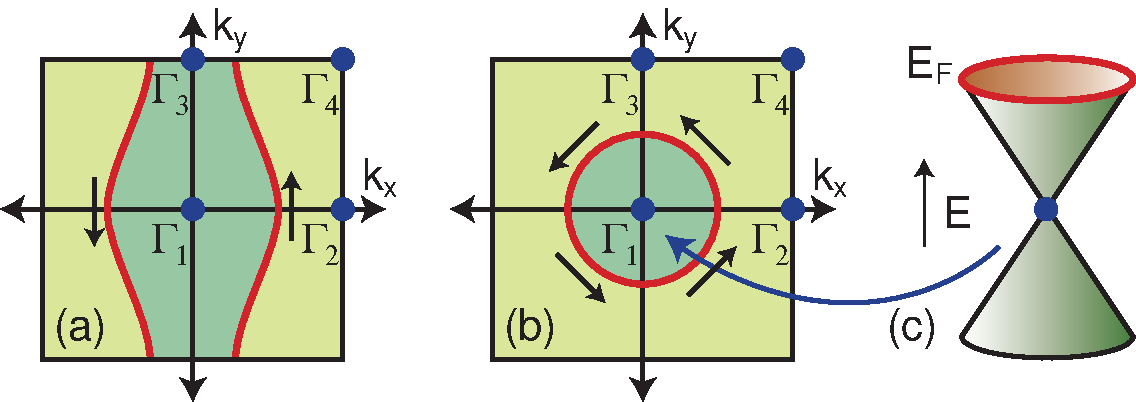
\includegraphics[width=3in]{Fig7}
		%\epsfxsize=3in
		%\epsfbox{Fig7.eps}
		\caption{Fermi circles in the surface Brillouin zone for (a) a weak topological insulator and
			(b) a strong topological insulator.  In the simplest strong topological insulator the Fermi circle
			encloses a single Dirac point (c).}
		\label{fig:surfacebz}
	\end{figure}
	
	The simplest non trivial 3D topological insulators may be
	constructed by stacking layers of the 2D quantum spin Hall
	insulator.  This is analogous to a similar construction for 3D
	integer quantum Hall states \cite{kohmoto92}.
	The helical edge states of the layers
	then become anisotropic surface states.
	A possible surface Fermi surface for weakly coupled layers stacked along the
	$y$ direction is sketched in Fig. \ref{fig:surfacebz}(a).  In this figure a single
	surface band intersects the Fermi energy between $\Gamma_1$ and $\Gamma_2$ and
	between $\Gamma_3$ and $\Gamma_4$, leading to the non trivial connectivity in
	Fig. \ref{fig:zigzag}(b).  This layered state is referred to as a weak topological
	insulator, and has $\nu_0=0$.
	The indices $(\nu_1\nu_2\nu_3)$ can be interpreted as Miller indices
	describing the orientation of the layers.
	Unlike the 2D helical edge states of a single layer, ${\cal T}$
	symmetry does not protect these surface states.  Though the
	surface states must be present for a clean surface, they
	can be localized in the presence of disorder.
	Interestingly, however, a line {\it dislocation} in
	a weak topological insulator is associated with protected 1D
	helical edge states \cite{ran09}.
	
	$\nu_0=1$ identifies a distinct phase, called a strong topological insulator,
	which can not be interpreted as a
	descendent of the 2D quantum spin Hall insulator.  $\nu_0$ determines
	whether an even or an odd number
	of Kramers points is enclosed by the surface Fermi circle.
	In a strong topological insulator the surface Fermi circle encloses an {\it odd} number of
	Kramers degenerate Dirac points.    The simplest case, with a single Dirac
	point(Fig. \ref{fig:surfacebz}(b,c)), can be described by the Hamiltonian,
	\begin{equation}
		{\cal H}_{\rm surface} = -i\hbar v_F \vec\sigma\cdot\vec\nabla,
		\label{surfacedirac}
	\end{equation}
	where $\vec\sigma$ characterizes the spin.  (For a surface with a mirror plane,
	symmetry requires $\vec S \propto \hat z\times\vec\sigma$.)
	
	The surface electronic structure of a topological insulator is
	similar to graphene, except rather than having four
	Dirac points (2 valley $\times$ 2 spin) there is just a single Dirac
	point.  This appears to violate the fermion doubling theorem \cite{nielssen83}
	discussed in section \ref{sec:dirac}.  The resolution is that the partner
	Dirac points reside on {\it opposite} surfaces.
	%The situation is
	%similar to the 2D quantum Hall effect, where the chiral edge states,
	%which violate a 1D doubling theorem, have a partner on the opposite
	%edge.
	
	The surface states of a strong topological insulator form a unique
	2D topological metal \cite{fukanemele07,fukane07} that is essentially {\it half}
	an ordinary metal.  Unlike an ordinary metal,
	which has up and down spins at every point on the Fermi surface, the surface
	states are not spin degenerate.  Since ${\cal T}$ symmetry requires that states at
	momenta ${\bf k}$ and $-{\bf k}$ have opposite spin, the spin must rotate with
	${\bf k}$ around the Fermi surface, as indicated in Fig.
	\ref{fig:surfacebz}(b).  This leads to a non trivial Berry phase
	acquired by an electron going around the Fermi
	circle.  ${\cal T}$ symmetry requires that this phase be $0$ or
	$\pi$.  When an electron circles a Dirac point, its spin rotates by
	$2\pi$, which leads to a $\pi$ Berry phase.
	
	The Berry phase has
	important consequences for the behavior in a magnetic field (to be
	discussed in section \ref{sec:qhetopomag}) and for the effects of disorder.  In
	particular, in an ordinary 2D electron gas the electrical
	conductivity decreases with decreasing temperature, reflecting the
	tendency towards Anderson localization in the presence of disorder \cite{lee85}.
	The $\pi$ Berry
	phase changes the sign of the weak localization correction to the
	conductivity leading to weak {\it antilocalization} \cite{suzuura02}.  In fact, the
	electrons at the surface of a strong topological insulator can not be
	localized even for strong disorder, as long as the bulk energy gap
	remains intact \cite{nomura07}.  In this regard, the situation is similar to the edge states of the
	quantum spin Hall insulator discussed in section \ref{sec:graphene}, however,
	the electron motion on the surface is diffusive rather than ballistic.
	
	The Dirac surface states \eqref{surfacedirac} can be
	understood in a 3D Dirac theory\cite{qihugheszhang08} where the Dirac mass changes sign at the
	surface, analogous to \eqref{jackiwrebbi}.  Such domain wall states were first
	discussed for Pb$_{1-x}$Sn$_x$Te\cite{volkov85,fradkin86},
	which exhibits a band inversion as a function of
	$x$.  An appropriate interface where $x$ changes was
	predicted to have 2D gapless states.  There is an important difference
	between these interface states and the surface
	states of a topological insulator, though, because the band inversion in
	Pb$_{1-x}$Sn$_x$Te occurs at 4 equivalent valleys.  Since 4 is even, PbTe and SnTe are
	both trivial insulators.  The interface states are not
	topologically protected from disorder in the sense discussed above.
	However, if the valleys can be split by applying uniaxial stress, then
	the topological insulator can occur in the vicinity of the band inversion
	transition\cite{fukane07}.
	Related ideas were also applied to interfaces between HgTe and CdTe
	\cite{chang85,cade85,linliu85,pankratovpakhomov87}.
	In this case, the band inversion occurs in a single valley, but since
	HgTe is a zero gap semiconductor, the surface states are not
	protected.  Nonetheless, if the cubic symmetry of the bulk HgTe can
	be lifted by applying uniaxial stress, a gap can be introduced in HgTe,
	so the HgTe-CdTe interface will have topologically protected states\cite{fukane07}.
	
	
	
	
	\subsection{The first 3D topological insulator: Bi$_{1-x}$Sb$_x$}
	\label{sec:bisb}
	
	\begin{figure}
		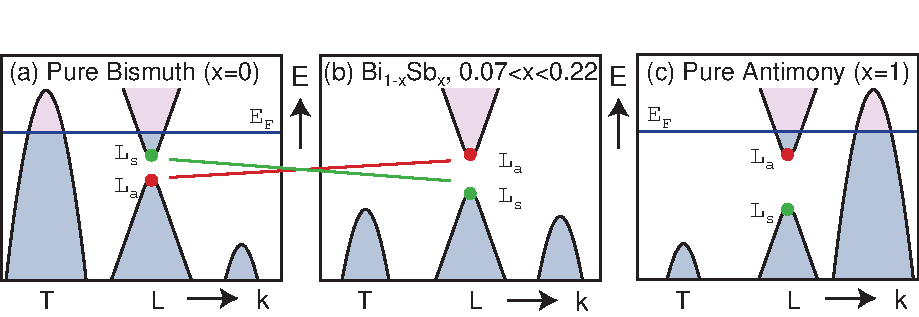
\includegraphics[width=3.2in]{Fig8}
		%\epsfxsize=3.2in
		%\epsfbox{Fig8.eps}
		\caption{Schematic representation of the band structure of Bi$_{1-x}$Sb$_x$,
			which evolves from semimetallic behavior for $x<.07$ to semiconducting behavior
			for $.07<x<.22$ and back to semimetallic behavior for $x>.18$.  The conduction
			and valence bands $L_{s,a}$ invert at $x \sim .04$. }
		\label{fig:bisbbands}
	\end{figure}
	\begin{table}
		\centering
		\begin{ruledtabular}
			\begin{tabular}{c|ccccc|c||c|ccccc|c}
				\multicolumn{7}{c||}{Bi: Class $(0;000)$ } &
				\multicolumn{7}{c}{Sb: Class $(1;111)$ } \\
				\multicolumn{1}{c}{$\Lambda_a$} &
				\multicolumn{5}{c}{Symmetry label}&
				\multicolumn{1}{c||}{$\delta_a$} &
				\multicolumn{1}{c}{$\Lambda_a$} &
				\multicolumn{5}{c}{Symmetry label} &
				\multicolumn{1}{c}{$\delta_a$} \\
				\hline
				$1\Gamma$ & $\Gamma_6^+$ & $\Gamma_6^-$ &$\Gamma_6^+$ &$\Gamma_6^+$ &
				$\Gamma_{45}^+$ & $-1$ &
				$1\Gamma$ & $\Gamma_6^+$ & $\Gamma_6^-$ &$\Gamma_6^+$ &$\Gamma_6^+$ &
				$\Gamma_{45}^+$ & $-1$ \\
				$3L$ & $L_s$ &$L_a$ &$L_s$ &$L_a$ &$L_a$ & $-1$ &
				$3L$ & $L_s$ &$L_a$ &$L_s$ &$L_a$ &$L_s$ & $+1$ \\
				$3X$ & $X_a$ & $X_s$ & $X_s$ & $X_a$ & $X_a$  & $-1$ &
				$3X$ & $X_a$ & $X_s$ & $X_s$ & $X_a$ & $X_a$  & $-1$ \\
				$1T$ & $T_6^-$ & $T_6^+$ & $T_6^-$ & $T_6^+$ & $T_{45}^-$ & $-1$ &
				$1T$ & $T_6^-$ & $T_6^+$ & $T_6^-$ & $T_6^+$ & $T_{45}^-$ & $-1$\\
			\end{tabular}
		\end{ruledtabular}
		\caption{Symmetry labels for the Bloch states at the 8 ${\cal T}$ invariant momenta
			$\Lambda_a$ for the 5 valence bands of Bi and Sb.
			$\delta_a$ are given by \eqref{parityz2} and
			determine the topological class $(\nu_0;\nu_1\nu_2\nu_3)$ by
			relations similar to \eqref{deltaa}.
			The difference between Bi and Sb is due to the inversion of
			the $L_s$ and $L_a$ bands that occurs at $x \sim .04$.}
		\label{tab:bisbtab}
	\end{table}
	
	The first 3D topological insulator to be identified experimentally
	was the semiconducting alloy
	Bi$_{1-x}$Sb$_{x}$, whose unusual surface bands were mapped in an
	angle resolved photoemission spectroscopy (ARPES) experiment by a Princeton
	University group led by Hasan\cite{hsieh08}.
	
	Bismuth antimony alloys have long been studied for their
	thermoelectric properties \cite{lenoir96}.  Pure bismuth is a semimetal with
	strong spin-orbit interactions.  Its band structure, depicted schematically in
	Fig. \ref{fig:bisbbands}(a) features conduction and valence bands that overlap,
	leading to pockets of holes near the $T$ point in the Brillouin zone
	and pockets of electrons near the three equivalent $L$ points.
	The valence and conduction bands at the $L$ point, derived
	from antisymmetric ($L_a$) and symmetric ($L_s$) orbitals have a small
	energy gap $\Delta$.  The states near $L$ have a nearly linear
	dispersion that is well described by a $3+1$
	dimensional Dirac equation \cite{wolff64} with a small mass.  These facts have been used to
	explain many peculiar properties of bismuth.
	
	Substituting bismuth with antimony changes the critical energies of
	the band structure (Fig. \ref{fig:bisbbands}(b)). At an Sb concentration of $x
	\approx .04$, the gap $\Delta$ between $L_a$ and $L_s$ closes and a
	truly massless 3D Dirac point is realized. As $x$ is
	further increased this gap reopens with an inverted ordering.
	For $x >.07$ the top of the valence band at $T$ moves below the bottom of the conduction
	band at $L$, and the material becomes an
	insulator. Once the band at $T$ drops below the valence band at $L$, at
	$x\sim .09$, the system is a direct gap insulator with
	a massive Dirac like bulk bands.  As $x$ is increased further, the conduction
	and valence bands remain separated, and for $x \gtrsim .22$ the valence band at
	a different point rises above the conduction band, restoring the semimetallic
	state.
	
	Since pure bismuth and pure antimony both have a finite direct band gap, their
	valence bands can be topologically classified.  Moreover, since they have
	inversion symmetry, Eq. \ref{parityz2} can be used to determine the topological indices.
	Table \ref{tab:bisbtab} shows the symmetry labels that specify the parity
	of the Bloch states, for the occupied bands at the 8
	${\cal T}$ invariant points in the bulk Brillouin zone \cite{liuallen95}.
	\textcite{fukane07} used this information to deduce
	that bismuth is in the trivial $(0;000)$ class, while antimony is in the
	$(1;111)$ class.  Since the semiconducting alloy is on the antimony side of the
	band inversion transition, it is predicted to inherit the $(1;111)$ class from
	antimony.
	
	Charge transport experiments,
	which were successful for identifying the 2D topological
	insulator \cite{konig07}, are problematic in 3D materials because
	the signature in the conductivity
	of the topological character of the surface states is more subtle in 3D.
	Moreover, it is difficult to separate the surface contribution to the conductivity
	from that of the bulk.
	Angle resolved photoemission spectroscopy (ARPES) is an ideal tool for probing
	the topological character of the surface states.
	ARPES uses a photon to eject an electron from a
	crystal, then determines the surface or bulk electronic structure
	from an analysis of the momentum of the emitted electron.
	High-resolution ARPES performed with
	modulated photon energy allows for a clear isolation of surface
	states from that of the bulk 3D band-structure because surface states
	do not disperse along a direction perpendicular to the surface where
	as the bulk states do. Moreover, unlike in a transport experiment,
	ARPES carried out in a spin resolution mode can, in addition, measure
	the distribution of spin orientations on the Fermi surface which can
	be used to estimate the Berry phase on the surface. Spin
	sensitivity is critically important for probing the existence of
	spin-momentum locking on the surface expected as a consequence of
	bulk topological order.
	
	\begin{figure}
		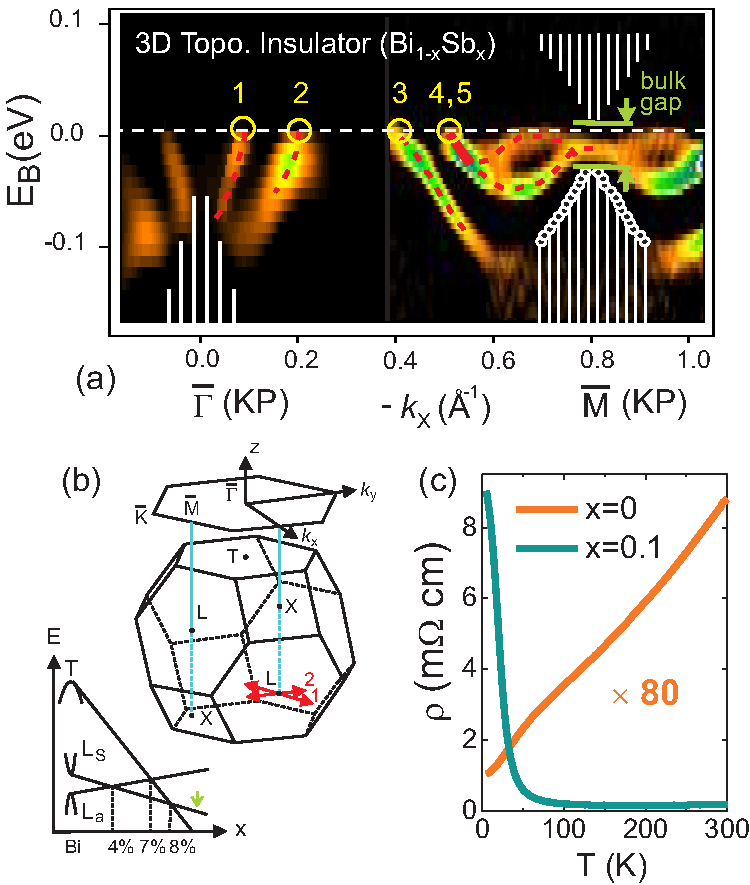
\includegraphics[width=2.8in]{Fig9}% Here is how to import EPS art
		\caption{Topological surface states in
			Bi$_{1-x}$Sb$_{x}$:  (a) ARPES data on the 111 surface of
			Bi$_{0.9}$Sb$_{0.1}$ which probes
			the occupied surface states as a function of momentum on the line connecting
			the ${\cal T}$ invariant points $\bar\Gamma$ and $\bar M$ in the surface Brillouin
			zone.  Only the surface bands cross the Fermi energy 5 times.  This, along with
			further detailed ARPES results \cite{hsieh08} establish that the semiconducting
			alloy Bi$_{1-x}$Sb$_{x}$ is a strong topological insulator in the $(1;111)$
			class.  (b) shows a schematic of the 3D Brillouin zone and its (111) surface
			projection.  (c) contrasts the resistivity of semimetallic pure Bi with
			the semiconducting alloy.  Adapted from \onlinecite{hsieh08}.}
		\label{fig:zfig1} \end{figure}
	
	Experiments by \textcite{hsieh08} probed both the bulk and
	surface electronic structure of Bi$_{.09}$Sb$_{.91}$ with ARPES.
	Fig. \ref{fig:zfig1}(a) shows the ARPES spectrum, which can be interpreted
	as a map of the energy of the occupied electronic states as a function
	of momentum along the line connecting $\bar\Gamma$ to $\bar M$ in the projected
	surface Brillouin zone (Fig. \ref{fig:zfig1}(b)).
	Bulk energy bands associated with the $L$ point are observed that reflect the
	nearly linear 3D Dirac like dispersion.
	The same experiments observed several surface states that span the bulk gap.
	
	The observed surface state structure of Bi$_{1-x}$Sb$_x$ has similarities with the
	surface states in pure Bi, which have been studied
	previously \cite{patthey94,agergaard01,ast01,hirahara06,hofmann06}.  In pure Bi, two
	bands emerge from the bulk band continuum near $\bar\Gamma$ to form a central
	electron pocket and an adjacent hole lobe.  These two bands result from the
	spin splitting of a surface state, and are thus expected to be singly
	degenerate.  In Bi$_{1-x}$Sb$_x$, there are additional states near $\bar M$,
	which play a crucial role.
	
	As explained in Section \ref{sec:strongweak}, Kramers' theorem requires surface states to be
	doubly degenerate at the ${\cal T}$ invariant points $\bar\Gamma$ and each of the
	three equivalent $\bar M$ points.
	Such a Kramers point is indeed observed at $\bar M$ approximately $15\pm 5$meV below
	$E_F$.  As expected for a system
	with strong spin orbit interactions, the degeneracy is lifted away from $\bar M$.
	The observed surface bands cross the Fermi energy 5 times between $\bar\Gamma$ and
	$\bar M$.  This odd number of crossings is analogous to Fig. \ref{fig:zigzag}(b),
	and indicates that these surface states are topologically protected.
	Accounting for the threefold rotational symmetry and mirror symmetry of the
	111 surface, this data shows that the surface Fermi surface encloses
	$\bar\Gamma$ an odd number of times, while it encloses the three equivalent
	$\bar M$ points an even number of times.  This establishes Bi$_{1-x}$Sb$_x$ as
	a strong topological
	insulator, with $\nu_0 = 1$.  The data is consistent with the predicted
	$(1;111)$ topological class.
	
	\begin{figure}
		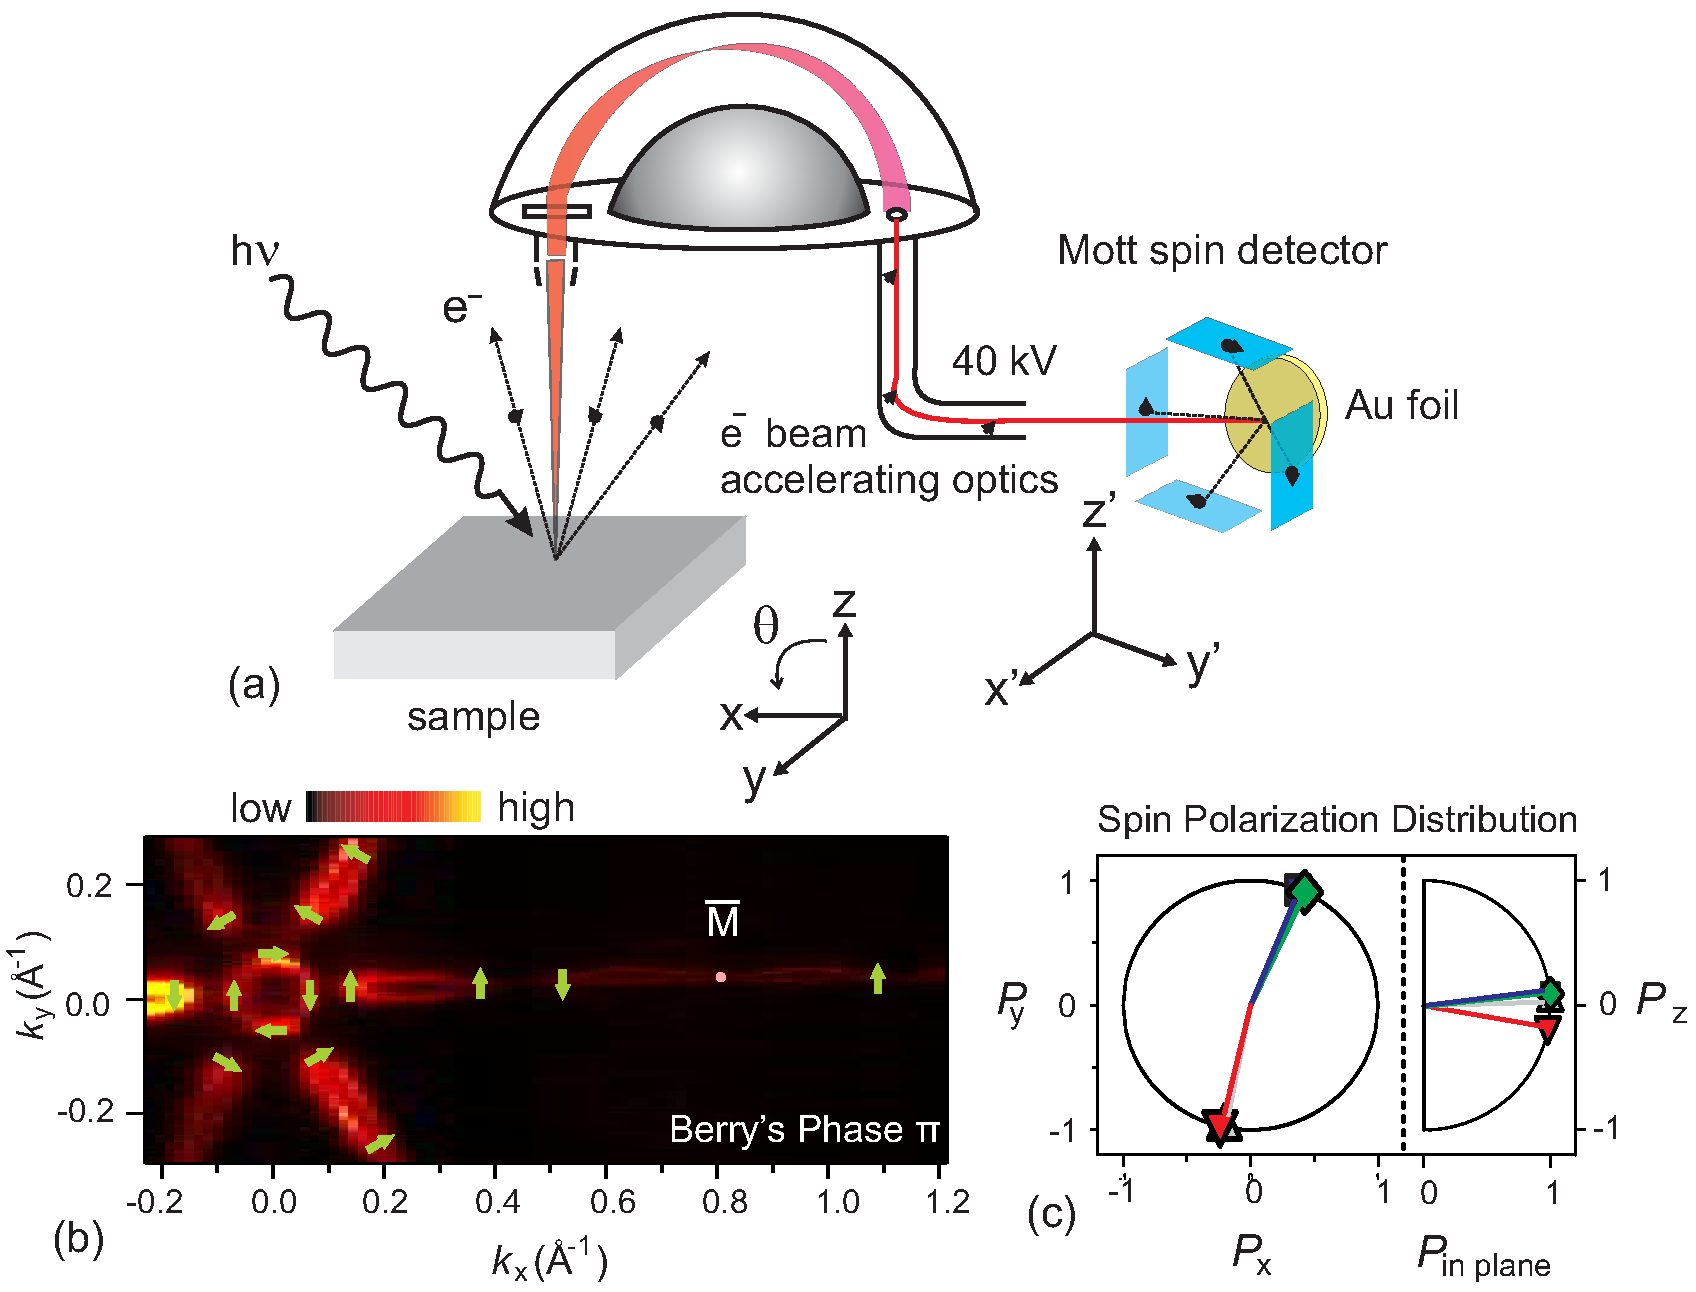
\includegraphics[width=3.3in]{Fig10}% Here is how to import EPS art
		\caption{Topological spin-textures:
			Spin resolved photoemission directly probes the non trivial spin textures
			of the topological insulator surface.
			(a) A schematic of spin-ARPES
			measurement set up that was used to measure the spin
			distribution on the (111) surface Fermi surface of
			Bi$_{0.91}$Sb$_{0.09}$.  (b) Spin orientations on the surface create a
			vortex like pattern around $\Gamma$-point. A net Berry phase
			$\pi$ is extracted from the full Fermi surface data.
			(c) Net polarization along x-, y- and z- directions are shown.
			\textit{P$_z$}$\sim$0 suggests that spins lie mostly within the
			surface plane.  Adapted from \onlinecite{hsieh09a,hsieh09d,hsieh10}.  }
		\label{fig:zfig2} \end{figure}
	
	A distinguishing feature of topological insulator surface states is the
	intimate correlation between spin and momentum they exhibit, which underlies
	the $\pi$ Berry phase associated with the Fermi surface.  Spin resolved
	ARPES, described schematically in Fig. \ref{fig:zfig2}(a),
	is ideally suited to probe this physics.
	Experiments by \textcite{hsieh09a} measured the spin polarization of the surface
	states.  These experiments proved that the surface states are indeed
	non degenerate and strongly spin polarized (Fig. \ref{fig:zfig2}(b)),
	providing even more decisive
	evidence for their topological classification.
	In addition, the spin polarization
	data also established the connectivity of the
	surfaces state bands above $E_F$ (which is inaccessible to ARPES),
	showing that bands labeled $2$ and $3$ in Fig. \ref{fig:zfig1}(a) connect to
	form a hole pocket.    Finally, they directly mapped
	the spin texture of the Fermi surface,
	providing the first direct evidence for
	the $\pi$ Berry phase by showing that the spin polarization rotates by
	$360^\circ$ around the central Fermi surface, shown in
	Fig. \ref{fig:zfig2}(c).  The measurement of the {\it handedness} of this
	rotation provided even more information about the topological structure,
	by probing a {\it mirror Chern number}, which agreed favorably with theory \cite{teofukane08}.
	
	Spin polarized ARPES also enables a similar characterization of
	surface states in the metallic regime of
	the Bi$_{1-x}$Sb$_x$ series.  Pure Sb is predicted to have a topologically non
	trivial valence band, despite the semi metallic band overlap.
	\textcite{hsieh09a} found that the surface states of Sb carry
	a Berry phase and chirality property predicted by theory \cite{teofukane08}
	that is unlike the conventional spin-orbit metals such as gold, which has
	zero net Berry phase and no net chirality.
	Additional compositions of the Bi$_{1-x}$Sb$_x$ series provided further
	evidence for the topological character of the surface states \cite{nishide10}.
	These results demonstrate that ARPES and spin-ARPES are powerful probes of topological
	order.
	
	\begin{figure}
		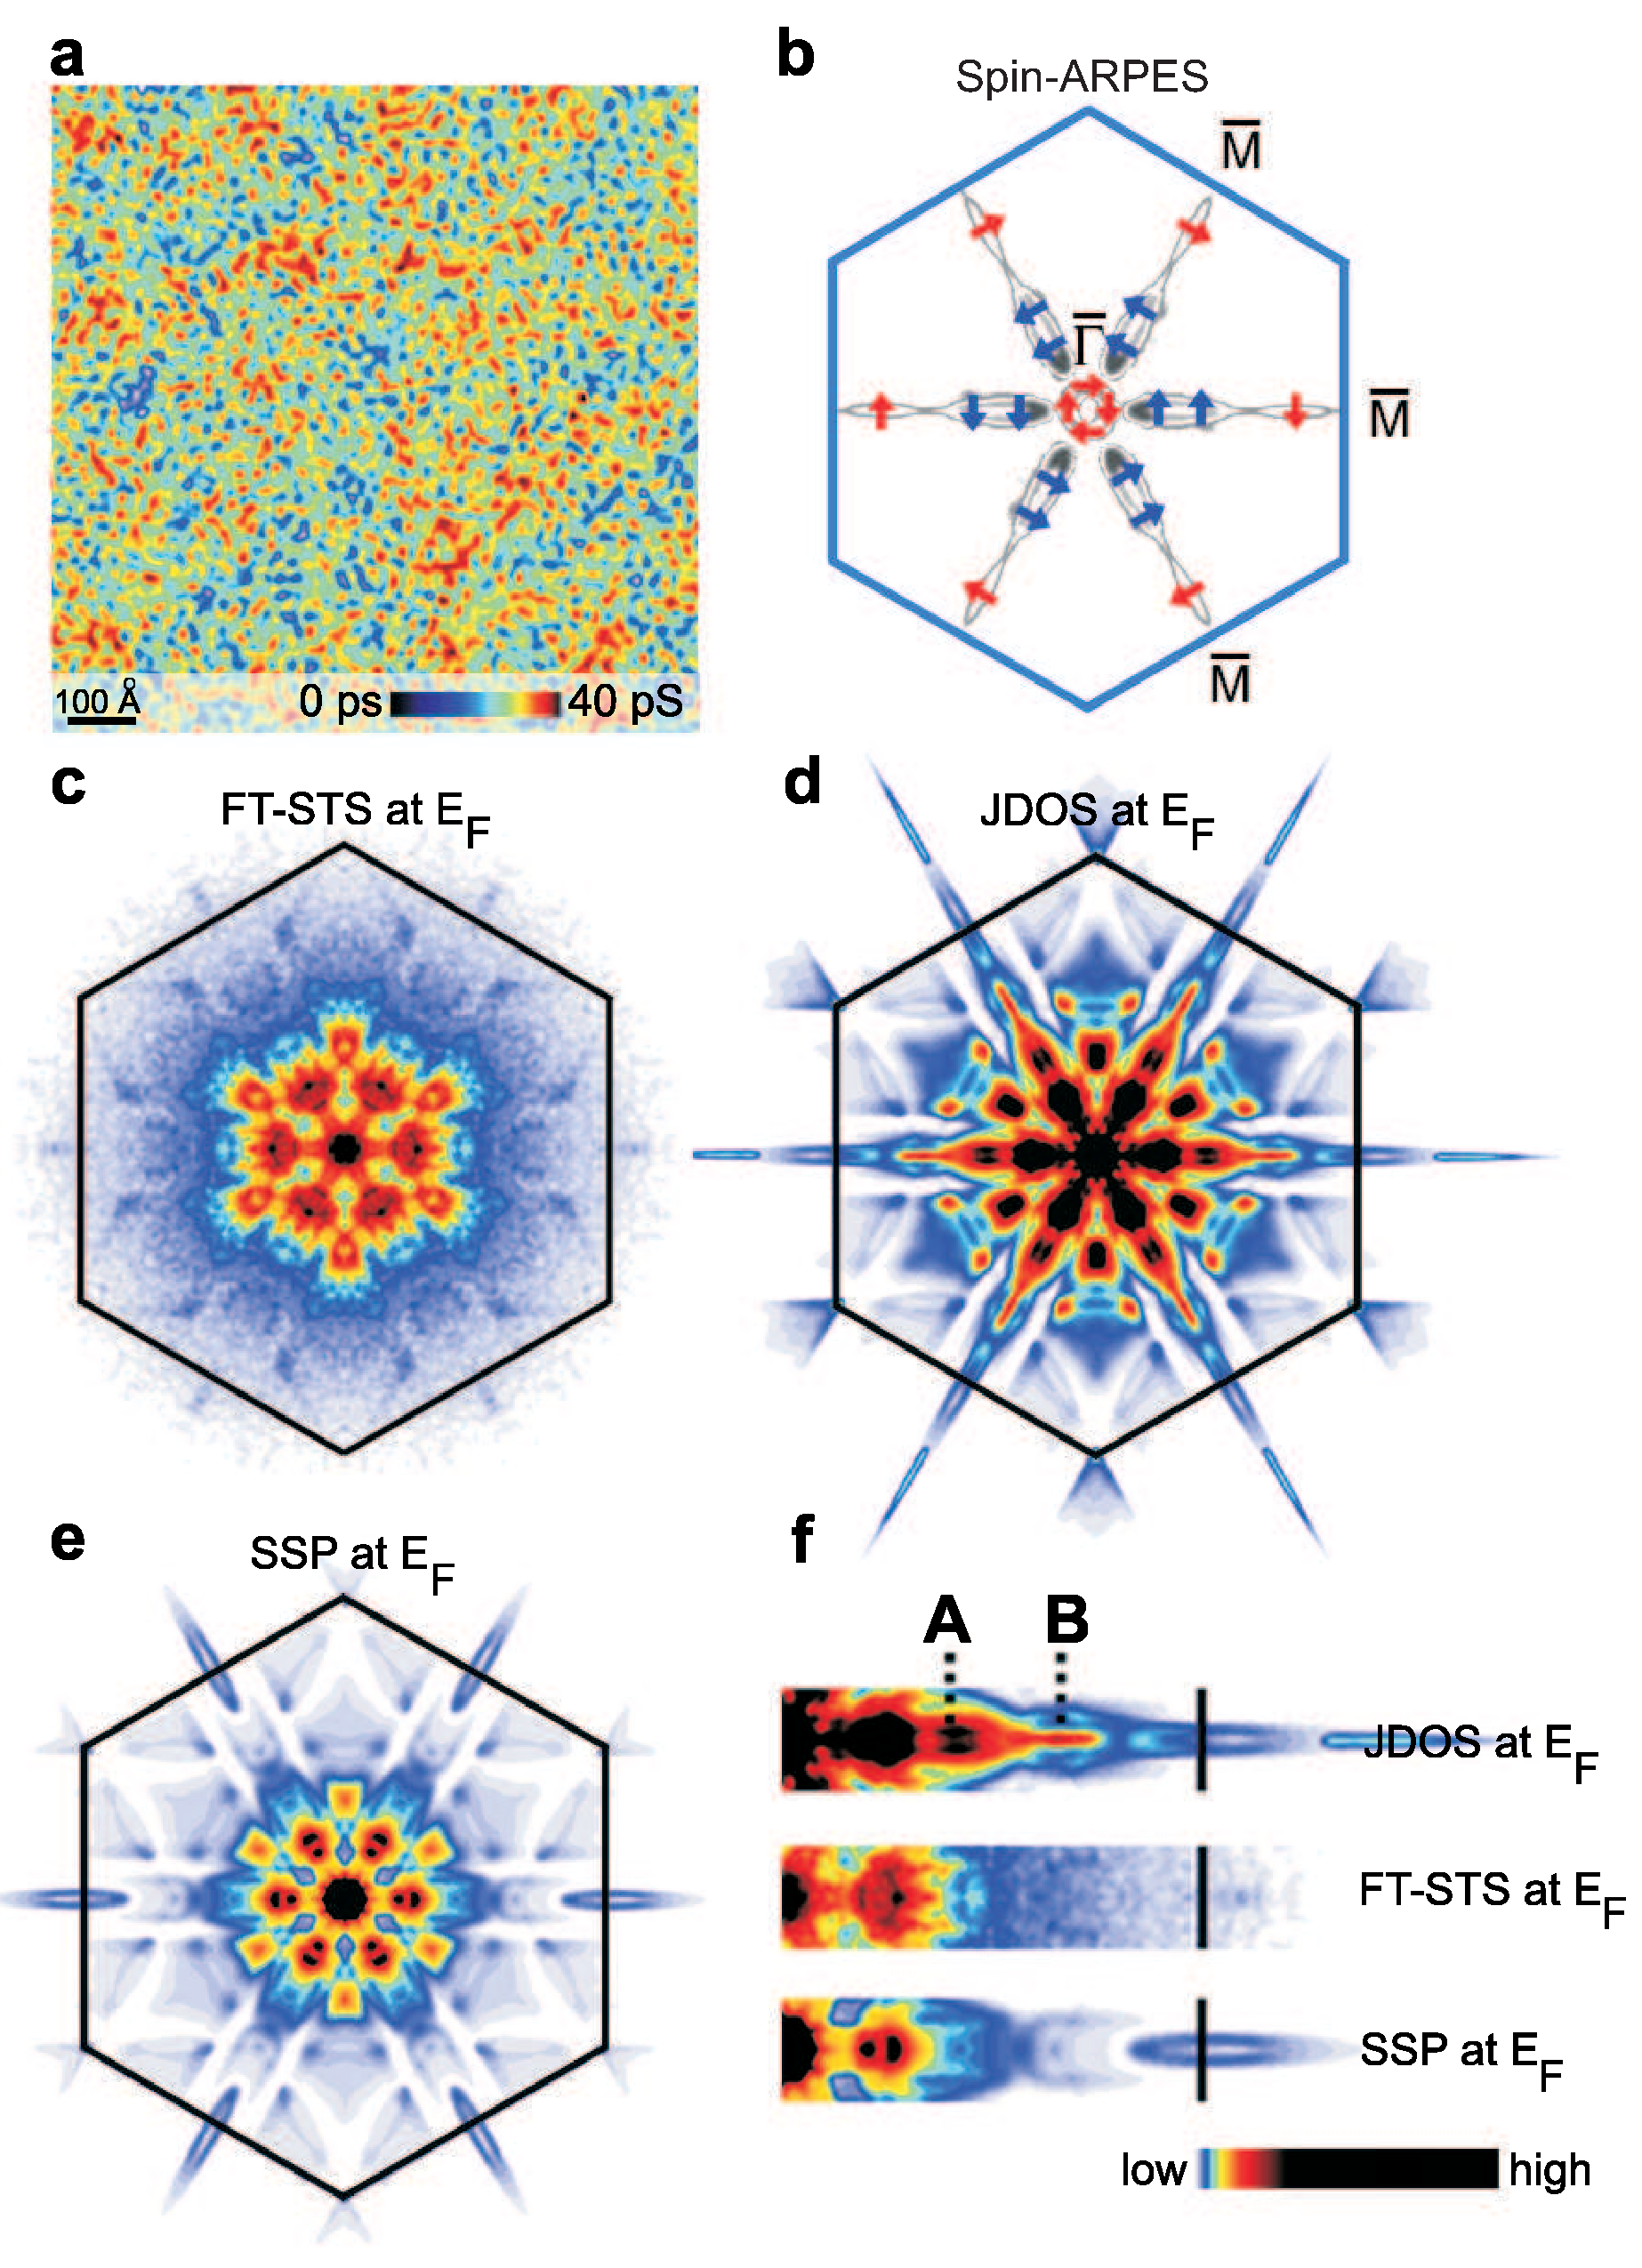
\includegraphics[width=2.8in]{Fig11}
		\caption{ Absence of backscattering:
			Quasiparticle interference observed at the surface of Bi$_{0.92}$Sb$_{0.08}$
			exhibits and
			absence of elastic backscattering: (a) Spatially resolved conductance
			maps of the (111) surface obtained at 0 mV
			over a 1000\AA$\times$1000\AA. (b) Spin-ARPES map of the
			surface state measured at the Fermi level. The spin textures from
			spin-ARPES measurements are shown with arrows. (c) Fourier transform
			scanning tunneling spectroscopy (FT-STS) at $E_F$. (d) The joint
			density of states (JDOS) at $E_F$. (e) The spin-dependent scattering
			probability(SSP) at $E_F$. (f) Close-up of the JDOS, FT-STS
			and SSP at $E_F$, along the $\Gamma$-M direction.  Adapted from
			\onlinecite{hsieh09a,roushan09}.}
		\label{fig:zfig3}
	\end{figure}
	
	As discussed in section \ref{sec:strongweak}
	the topological surface states are expected to be
	robust in the presence of non magnetic disorder, and immune from
	Anderson localization.  The origin of this is the fact that
	${\cal T}$ symmetry forbids the backscattering between Kramers
	pairs at ${\bf k}$ and $-{\bf k}$.
	Random alloying in Bi$_{1-x}$Sb$_x$,
	which is not present in other material families of topological
	insulators found to date, makes this material system an ideal
	candidate in which to examine the impact of disorder or random
	potential on topological surface states. The fact that the
	2D states are indeed protected from spin-independent
	scattering was established by \textcite{roushan09} by
	combining results from scanning tunneling spectroscopy and
	spin-ARPES.  Fig. \ref{fig:zfig3} shows
	the analysis of the interference pattern
	due to scattering at the surface.
	Fig. \ref{fig:zfig3}(c) shows the Fourier transform of the observed pattern
	(Fig. \ref{fig:zfig3}(a)),
	while Figs. \ref{fig:zfig3}(d,e) show the joint density of states computed from
	the Fermi surface (Fig. \ref{fig:zfig3}(b))
	with and without a suppression of ${\bf k}$ to $-{\bf k}$
	backscattering.  The similarity between Figs. \ref{fig:zfig3}(c,e) shows that
	despite strong atomic scale disorder,
	${\bf k}$ to $-{\bf k}$ backscattering is absent.
	Similar conclusions have emerged from studies of the electronic interference
	patterns near defects or steps on the surface in other topological insulators
	\cite{urazhdin04,zhangt09,alpichshev10}.  In graphene there is an approximate version of
	this protection if the disorder has a smooth potential which does
	not mix the valleys at ${\bf K}$ and ${\bf K}'$, but real graphene
	will become localized with strong disorder \cite{neto09}.
	
	\subsection{Second generation materials: Bi$_2$Se$_3$, Bi$_2$Te$_3$, Sb$_2$Te$_3$}
	\label{sec:bise}
	
	The surface structure of Bi$_{1-x}$Sb$_x$ was
	rather complicated and the band gap was rather small.  This
	motivated a search for topological insulators with a larger band gap
	and simpler surface spectrum.
	A second generation of 3D
	topological insulator materials \cite{moore09}, especially Bi$_2$Se$_3$, offer the
	potential for topologically protected behavior in ordinary crystals
	at room temperature and zero magnetic field.
	%This is in stark contrast to the quantum Hall effect,
	%which generally requires low temperature and strong magnetic fields.
	In 2008, work led by the Princeton group used ARPES and
	first principles calculations to study the surface band structure of
	Bi$_2$Se$_3$ and observed the characteristic signature of a
	topological insulator in the form of a single Dirac cone \cite{xia09a}.
	Concurrent theoretical work by \textcite{zhangh09}
	used electronic structure methods to show that
	Bi$_2$Se$_3$ is just one of several new large band gap topological
	insulators. \textcite{zhangh09} also provided a simple tight-binding
	model to capture the single Dirac cone observed in these materials.
	Detailed and systematic surface
	investigations of Bi$_2$Se$_3$ \cite{hsieh09b,hor09,park10}, Bi$_2$Te$_3$
	\cite{chen09,hsieh09b,hsieh09c,xia09b} and  Sb$_2$Te$_3$ \cite{hsieh09c}
	confirmed the topological band structure of all 3 of these materials.
	This also explained earlier
	puzzling observations on Bi$_2$Te$_3$ \cite{noh08}.
	These works showed that the topological insulator behavior in
	these materials is associated with a band inversion at ${\bf k}=0$, leading to
	the $(1;000)$ topological class.
	The $(1;000)$ phase observed in the Bi$_2$Se$_3$ series
	differs from the $(1;111)$ phase in Bi$_{1-x}$Sb$_x$ due to its
	weak topological invariant, which has implications for the behavior
	of dislocations\cite{ran09}.
	
	\begin{figure}
		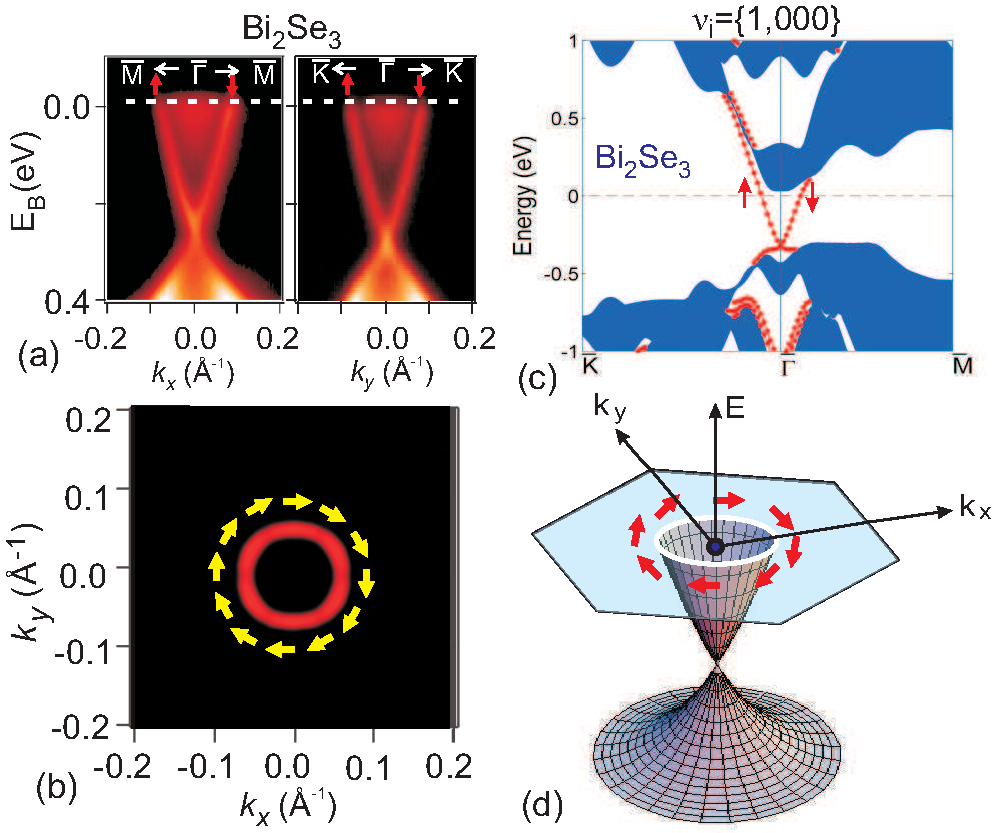
\includegraphics[width=3in]{Fig12}
		\caption{\label{fig:zfig4}
			Helical fermions: Spin-momentum
			locked helical surface Dirac fermions are hallmark signatures of
			topological insulators.  (a) ARPES data for Bi$_2$Se$_3$ reveals
			surface electronic states with a single
			spin-polarized Dirac cone. The Surface Fermi surface (b) exhibits a chiral
			left-handed spin texture.  (c) Surface electronic structure of
			Bi$_2$Se$_3$ computed in the local density approximation.  The shaded
			regions describe bulk states, and the red lines are surface states.
			(d) Schematic of the spin polarized surface state dispersion in
			Bi$_2$X$_3$ $(1;000)$ topological insulators.  Adapted from \onlinecite{hsieh09b,xia08,xia09b}.}
	\end{figure}
	
	Though the phase observed in the Bi$_2$Se$_3$ class has the same
	strong topological invariant $\nu_0=1$ as Bi$_{1-x}$Sb$_x$,
	there are three
	crucial differences that suggest that this series may become the
	reference material for future experiments. The
	Bi$_2$Se$_3$ surface state is found from ARPES and theory to be
	a nearly idealized single Dirac cone as seen from the experimental
	data in Figs. \ref{fig:zfig4},\ref{fig:zfig7},\ref{fig:zfig6}.
	Second, Bi$_2$Se$_3$ is stoichiometric (i.e., a pure
	compound rather than an alloy like Bi$_{1-x}$Sb$_x$) and hence can be
	prepared in principle at higher purity.  While the topological
	insulator phase is predicted to be quite robust to disorder, many
	experimental probes of the phase, including ARPES of the surface band
	structure, are clearer in high-purity samples. Finally, and perhaps
	most important for applications, Bi$_2$Se$_3$ has a large band gap of
	approximately 0.3 eV (3600$^\circ$K).  This indicates that in its high
	purity form Bi$_2$Se$_3$ can exhibit topological insulator behavior at
	{\it room temperature}(Fig. \ref{fig:zfig7})
	and greatly increases the
	potential for applications. To understand the likely impact
	of these new topological insulators, an analogy can be drawn with the
	early days of high-temperature cuprate superconductivity: the
	original cuprate superconductor LBCO was quickly superseded by
	``second-generation" materials such as YBCO and BSCCO for most applied
	and scientific purposes.
	
	\begin{figure}
		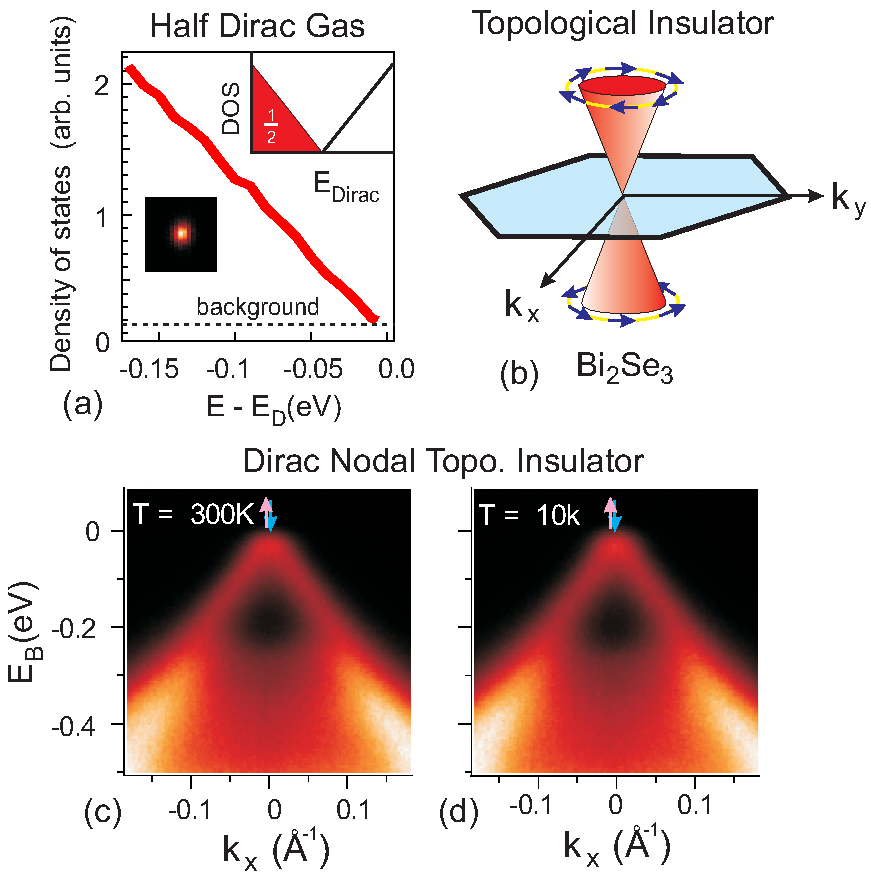
\includegraphics[width=3in]{Fig13}
		\caption{ Room temperature topological
			order in Bi$_2$Se$_3$:  (a) Crystal momentum
			integrated ARPES data near Fermi level exhibit linear fall-off of
			density of states, which combined with the spin-resolved nature of
			the states suggest that a half Fermi gas is realized on the
			topological surfaces. (b) Spin-texture map based on spin-ARPES data
			suggest that the spin-chirality changes sign across the Dirac point.
			(c) The Dirac node remains well
			defined up a temperature of 300K suggesting the stability of
			topological effects up to the room temperature.  Adapted from \onlinecite{hsieh09b}.}
		\label{fig:zfig7}
	\end{figure}
	
	All the key properties of
	topological states have been demonstrated for Bi$_2$Se$_3$ which has
	the simplest Dirac cone surface spectrum and the largest band gap.
	In Bi$_2$Te$_3$ the surface states exhibit large deviations
	from a simple Dirac cone (Fig. \ref{fig:zfig8}) due to a combination of smaller
	band gap (0.15 eV) and a strong trigonal potential \cite{chen09},
	which can be utilized to explore some aspects
	of its surface properties \cite{fu09,hasan09}.
	The hexagonal deformation of the surface states is confirmed by STM
	measurements \cite{alpichshev10} (Fig. \ref{fig:zfig8}).
	Speaking of applications within this class of
	materials, Bi$_2$Te$_3$, is already well known to materials
	scientists working on thermoelectricity.  It is a commonly used
	thermoelectric material in the crucial engineering regime near room
	temperature.
	
	\begin{figure}
		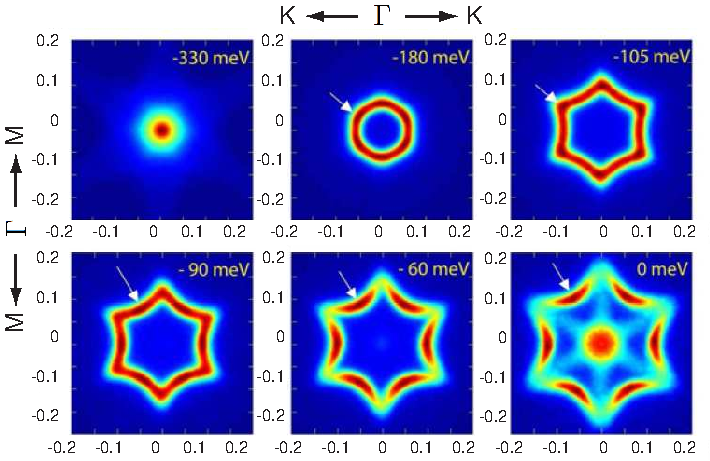
\includegraphics[width=3in]{Fig14}
		\caption{Hexagonal warping of
			surface states in Bi$_2$Te$_3$: ARPES and STM studies of Bi$_2$Te$_3$
			reveal a hexagonal deformation of surface states.  Fermi surface evolution with
			increasing n-type doping as observed in ARPES measurements.  Adapted from
			\onlinecite{alpichshev10}.}
		\label{fig:zfig8}
	\end{figure}
	
	Two defining properties of topological insulators --
	spin-momentum locking of surface states and $\pi$ Berry phase -- can
	be clearly demonstrated in the Bi$_2$Se$_3$ series.
	The surface states are expected to be protected by ${\cal T}$ symmetry
	which implies that the surface Dirac node should be robust in
	the presence of non-magnetic disorder but open a gap in the presence
	of ${\cal T}$ breaking perturbations.
	Magnetic impurities such as Fe or Mn on the surface of Bi$_2$Se$_3$ open a gap at the
	Dirac point (Fig. \ref{fig:zfig5}(a,b)) \cite{xia08,hsieh09b,hor10b,wray10}.
	The magnitude of the gap is
	likely set by the interaction of Fe ions with the Se surface and the
	${\cal T}$ breaking disorder potential introduced on the surface.
	Non-magnetic disorder created via molecular absorbent NO$_2$ or
	alkali atom adsorption (K or Na) on the surface leaves the Dirac node
	intact (Fig. \ref{fig:zfig5}(c,d)) in both Bi$_2$Se$_3$ and Bi$_2$Te$_3$
	\cite{xia09b,hsieh09b}. These results
	are consistent with the fact that the topological surface states are
	protected by ${\cal T}$ symmetry.
	
	\begin{figure}
		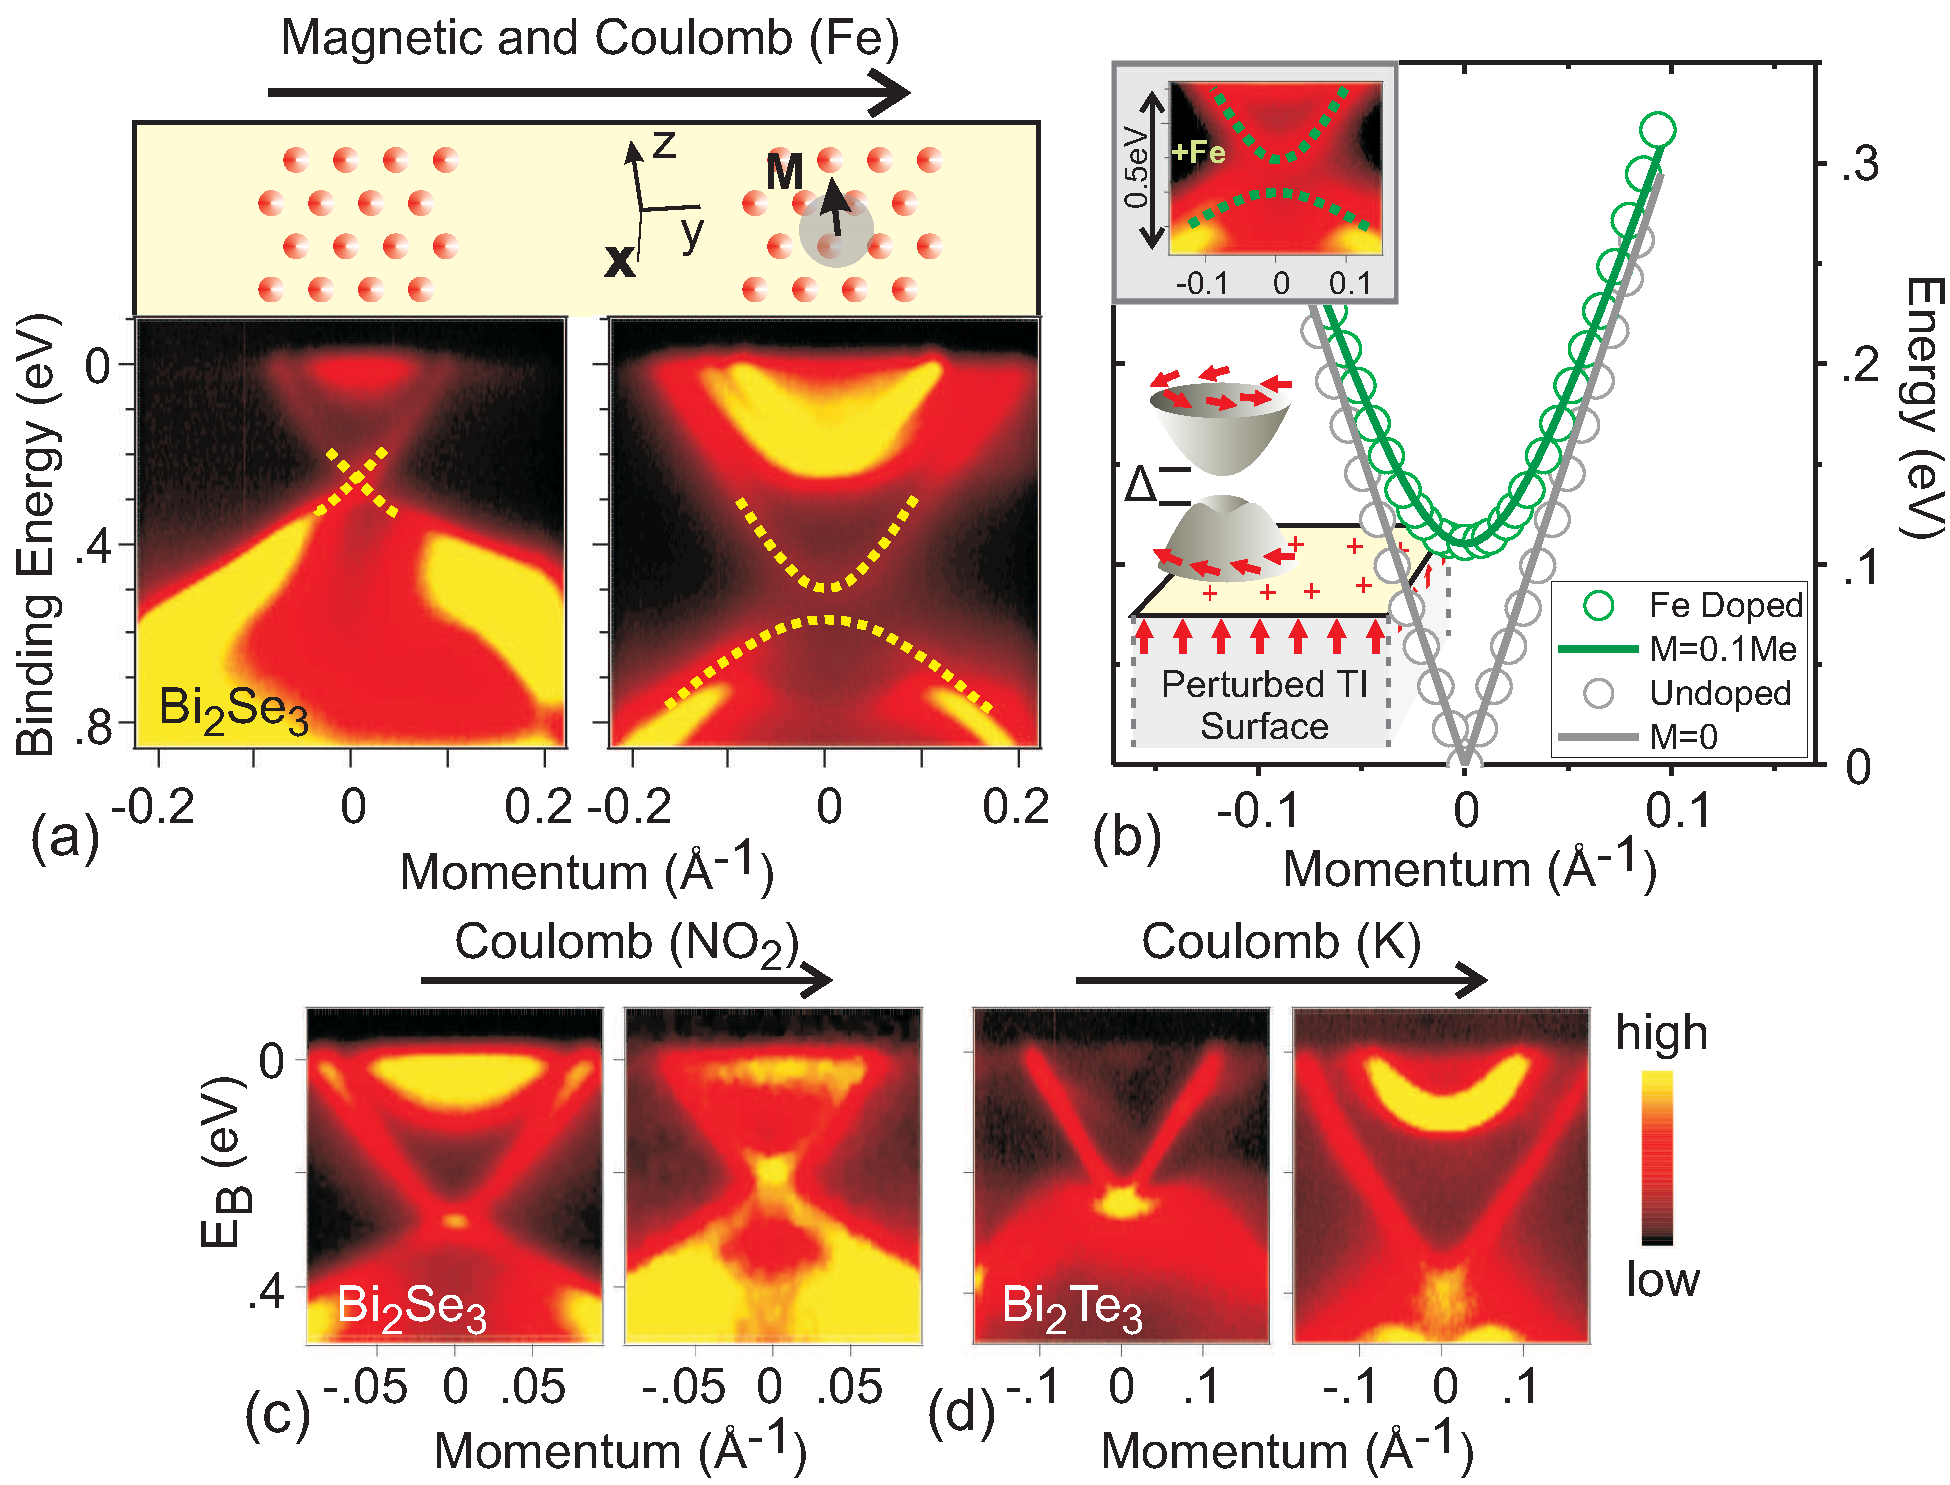
\includegraphics[width=3in]{Fig15}% Here is how to import EPS art
		\caption{ Protection by time reversal
			symmetry: Topological surface states are robust in the presence of
			strong non-magnetic disorder but open a gap in the presence of
			${\cal T}$ breaking magnetic impurities and disorder. (a) Magnetic
			impurity such as Fe on the surface of Bi$_2$Se$_3$ opens a gap at the
			Dirac point. The magnitude of the gap is set by the interaction of Fe
			ions with the Se surface and the ${\cal T}$ breaking disorder
			potential introduced on the surface. (b) A comparison of surface band
			dispersion with and without Fe doping. (c,d) Non-magnetic disorder
			created via molecular absorbent NO$_2$ or alkali atom adsorption (K
			or Na) on the surface leaves the Dirac node intact in both
			Bi$_2$Se$_3$ and Bi$_2$Te$_3$.  Adapted from \onlinecite{hsieh09b,xia09b,wray10}.}
		\label{fig:zfig5}
	\end{figure}
	
	\begin{figure}
		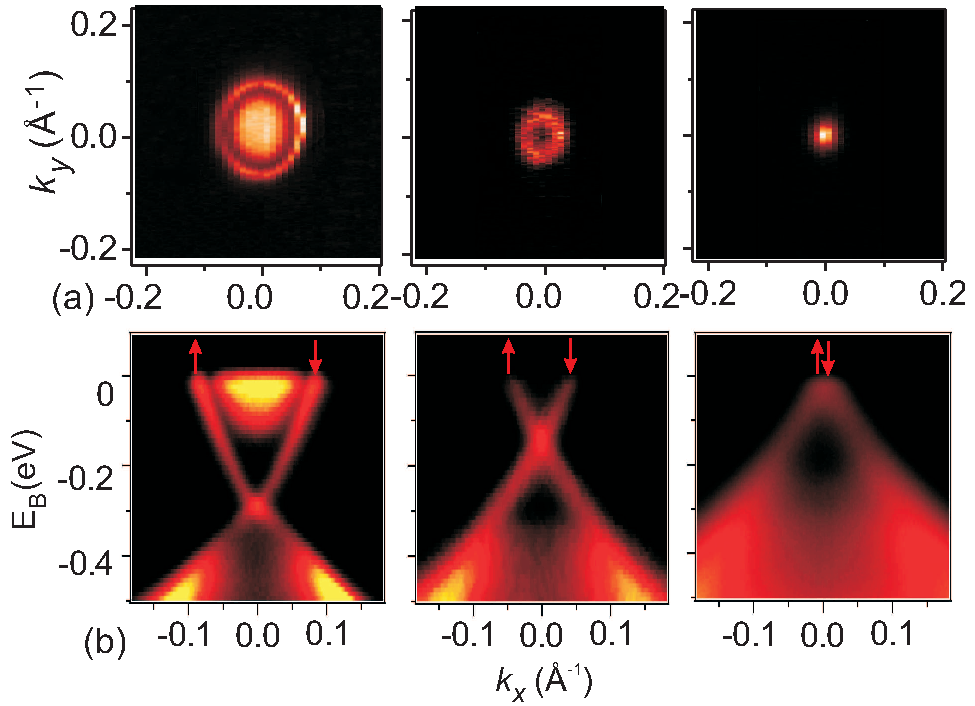
\includegraphics[width=3in]{Fig16}% Here is how to import EPS art
		\caption{
			Chemical gating a topological
			surface to the spin-degenerate point: Topological insulator surfaces
			are most interesting if the chemical potential can be placed at the
			Dirac node without intercepting any bulk band. This can be
			achieved in Bi$_2$Se$_3$ via the chemical tailoring of the surface or
			using electrical gating methods. (a) Evolution of surface Fermi
			surface with increasing NO$_2$ adsorption on the surface.
			NO$_2$ extracts electrons from the Bi$_2$Se$_3$ surface leading to an
			effective hole doping of the material. (b) Chemical gating of the
			surface can be used to place the chemical potential at the spin
			degenerate Dirac point.  Adapted from \onlinecite{hsieh09b}.}
		\label{fig:zfig6}
	\end{figure}
	
	Many of the interesting theoretical proposals that utilize
	topological insulator surfaces
	require the chemical potential to lie at or near the surface Dirac point.
	This is similar to the case in graphene, where
	the chemistry of carbon atoms naturally locates the Fermi
	level at the Dirac point.   This makes its
	density of carriers highly tunable by an applied electrical field and
	enables applications of graphene to both basic science and
	microelectronics.  The surface Fermi level of a topological insulator
	depends on the detailed electrostatics of the surface, and is not necessarily
	at the Dirac point.  Moreover, for naturally grown Bi$_2$Se$_3$ the {\it bulk} Fermi
	energy is not even in the gap.  The observed $n$ type behavior is believed to
	be caused Se vacancies.  By appropriate chemical modifications, however, the
	Fermi energy of both the bulk and the surface can be controlled.
	This allowed \textcite{hsieh09b} to reach the sweet spot in which the surface
	Fermi energy is tuned to the Dirac point (Fig. \ref{fig:zfig6}).  This
	was achieved by doping bulk
	with a small concentration of Ca,
	which compensates the Se vacancies, to place the Fermi level within
	the bulk band gap.  The surface was hole doped by exposing the
	surface to NO$_2$ gas to place the Fermi level at the Dirac point.
	
	The main remaining complication with these materials, especially for
	experimental techniques that (unlike ARPES) do not distinguish
	directly between bulk and surface states, is that they have some
	residual conduction in the bulk from impurity or self doping states.
	Electrical transport measurements on Bi$_2$Se$_3$ show that doping with a small
	concentration of Ca leads to insulating behavior.  Fig. \ref{fig:transport}(a)
	shows the resistivity of several samples with varying Ca concentrations.  For
	$.002<x<.025$, the resistivity shows a sharp upturn below 100$^\circ$K before
	saturating.  The low temperature resistivity is still too small to be explained by
	the surface states alone.  However, the low temperature transport exhibits
	interesting 2D mesoscopic effects that are not completely
	understood \cite{checkelsky09}.   Doping Bi$_2$Se$_3$ with copper leads to a
	metallic state that shows superconducting behavior (Fig.
	\ref{fig:transport}(b)) below 3.8$^\circ$K \cite{hor10a,wray09}.  This has important
	ramifications for some of the devices proposed in the following section.
	
	\begin{figure}
		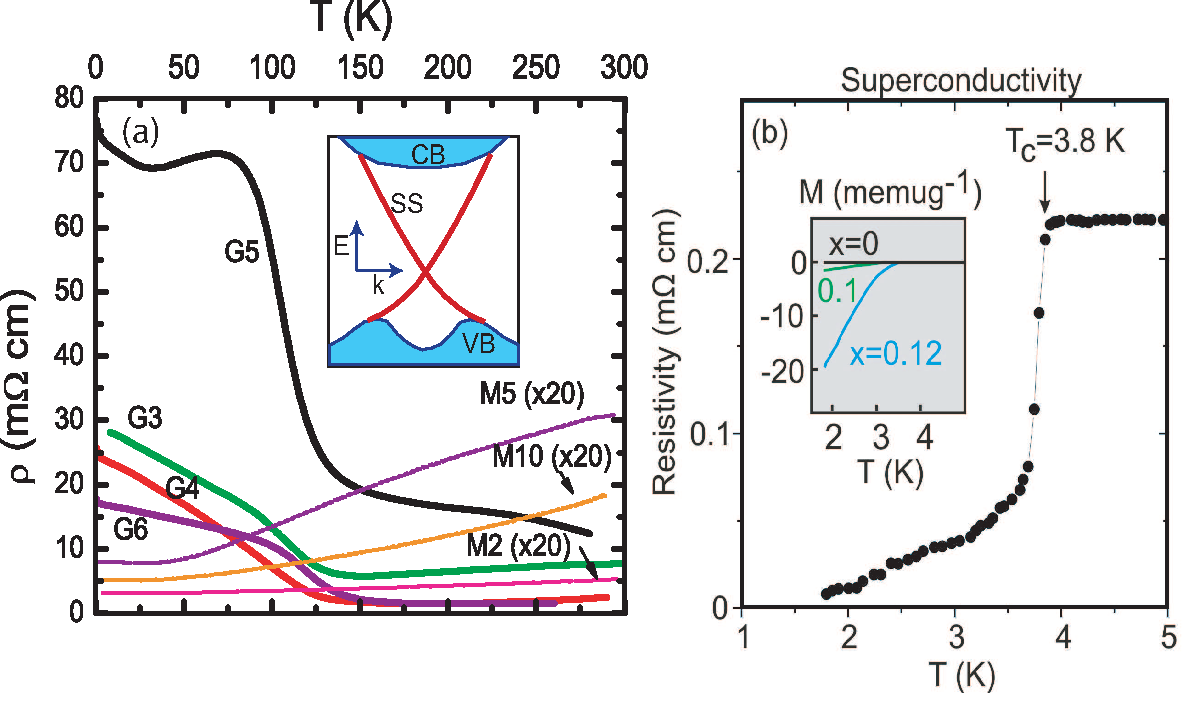
\includegraphics[width=3in]{Fig17}% Here is how to import EPS art
		\caption{Electrical transport in Bi$_2$Se$_3$.  (a) Resistivity for samples of
			pure Bi$_2$Se$_3$ doped with a small concentration of Ca.  Increasing the Ca
			concentration moves the Fermi level from the conduction band into the gap and
			then to the valence band.  Samples with $.002<x<.0025$, labeled G,
			show insulating behavior below 100$^\circ$K \cite{checkelsky09}.  (b) Bi$_2$Se$_3$ doped with Cu shows superconducting behavior
			below 3.8$^\circ$K for $x = .12$.  The inset shows the magnetic susceptibility
			which exhibits the Meissner effect.  Adapted from \onlinecite{hor10a,wray10}.
		}
		\label{fig:transport}
	\end{figure}
	
	\section{Exotic Broken Symmetry Surface Phases}
	\label{sec:exoticsurface}
	
	Now that the basic properties of topological insulators have been established,
	we may ask what can be done with them.  In this section we will argue
	that the unique properties of topological insulator surface and edge
	states are most dramatic if an energy gap can be induced in them.
	This can be done by breaking ${\cal T}$ symmetry with an external
	magnetic field \cite{fukane07} or proximity to a magnetic material \cite{qihugheszhang08}, by breaking gauge
	symmetry due to proximity to a superconductor \cite{fukane08}, or by an excitonic
	instability of two coupled surfaces \cite{seradjeh09}.  In this section we review
	the magnetic and superconducting surface phases.
	
	\subsection{Quantum Hall effect and topological magnetoelectric effect}
	\label{sec:qhetopomag}
	
	\subsubsection{Surface quantum Hall effect}
	\label{sec:surfaceqhe}
	
	A perpendicular magnetic field will lead to Landau levels in the
	surface electronic spectrum, and the quantum Hall effect.
	The Landau levels for Dirac electrons
	are special, however, because a Landau level is guaranteed to exist
	at exactly zero energy \cite{jackiw84}.  This zero Landau level is particle-hole symmetric
	in the sense that the Hall conductivity is equal and opposite when the
	Landau level is full or empty.  Since the Hall conductivity increases by
	$e^2/h$ when the Fermi energy crosses a Landau level
	the Hall conductivity is {\it half integer} quantized \cite{ando02},
	\begin{equation}
		\sigma_{xy} = (n+1/2) e^2/h.
		\label{n+1/2}
	\end{equation}
	
	This physics has been famously demonstrated in experiments on
	graphene \cite{novoselov05,zhangy05}.  However, there is an important difference.  In graphene
	\eqref{n+1/2} is multiplied by four, due to the spin and valley degeneracy
	of graphene's Dirac points, so the observed Hall conductivity is
	still integer quantized.  At the surface of the topological
	insulator there is only a {\it single} Dirac point.  Such a
	``fractional" integer quantized Hall effect should be a cause for
	concern because the integer quantized Hall effect is always
	associated with chiral edge states, that can only be integer
	quantized.  The resolution is the mathematical fact
	that a surface can not have
	a boundary.  In a slab geometry shown in Fig. \ref{fig:surfaceqhe}(a), the
	top surface and bottom surface are necessarily connected to each other, and will
	always be measured in parallel \cite{fukane07}, doubling the $1/2$.  The top and
	bottom can share a single chiral edge state, which carries the integer
	quantized Hall current.
	
	\begin{figure}
		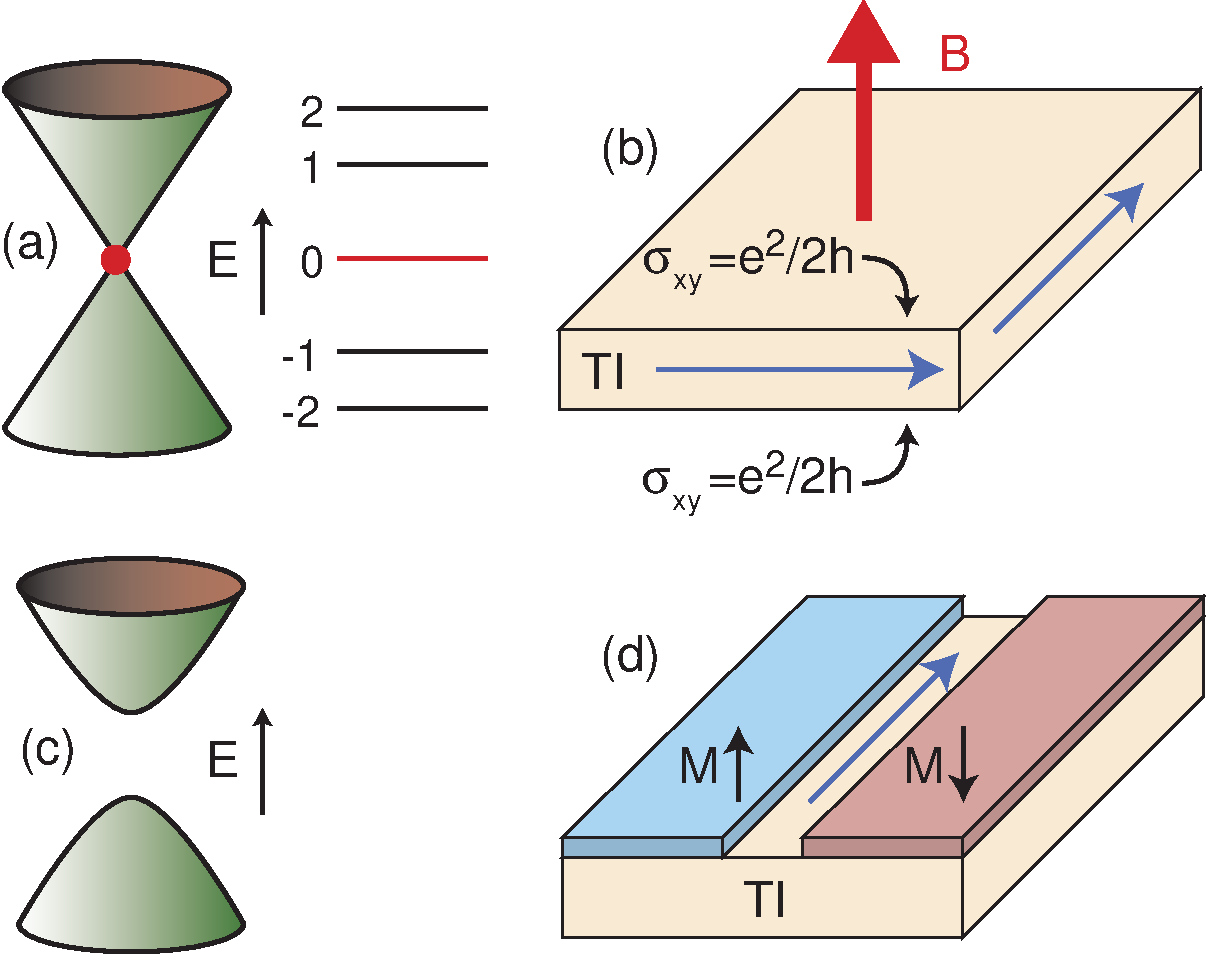
\includegraphics[width=2.8in]{Fig18}
		\caption{Surface quantum Hall effect.  (a) The Dirac spectrum is replaced by Landau levels
			in an orbital magnetic field.  (b) The top and bottom surfaces share a single chiral fermion
			edge mode.  (c) A thin magnetic film can induce an energy gap at the surface.
			(d) A domain wall in the surface magnetization then exhibits a chiral fermion mode.}
		\label{fig:surfaceqhe}
	\end{figure}
	
	A related surface quantum Hall effect, called the anomalous quantum Hall
	effect, can be induced with the proximity to a
	magnetic insulator.  A thin magnetic
	film on the surface of a topological insulator will give rise to a local exchange
	field that lifts the Kramers degeneracy at the surface Dirac points.  This
	introduces a mass term $m$ into the Dirac equation \eqref{surfacedirac},
	as in \eqref{diracmass}.  If the $E_F$ is in this energy
	gap, there is a half integer quantized Hall conductivity
	$\sigma_{xy}=e^2/2h$\cite{pankratov87}, as discussed in section \ref{sec:dirac}.
	This can be probed in a transport experiment by introducing a {\it domain
		wall} into the magnet.  The sign of $m$ depends on the direction of
	the magnetization.  At an interface where $m$ changes sign (Fig. \ref{fig:surfaceqhe}(d))
	there will be a 1D chiral edge state, analogous to unfolding the
	surface in Fig. \ref{fig:surfaceqhe}(b).
	%The presence of these edge states can then be probed with
	%non local transport experiments.
	
	\subsubsection{Topological magnetoelectric effect and axion electrodynamics}
	\label{sec:topomag}
	
	The surface Hall conductivity can also be probed without the
	edge states either by optical methods or by measuring the magnetic field produced by surface
	currents.  This leads to an intriguing {\it topological magnetoelectric effect} \cite{qihugheszhang08,essin09}.
	Imagine a cylindrical topological insulator with magnetically gapped surface
	states and an electric field ${\bf E}$ along its axis.  The azimuthal surface Hall
	current $(e^2/2h)|{\bf E}|$ leads to a magnetic dipole moment associated
	with a magnetization ${\bf M} = \alpha{\bf E}$, where the magnetoelectric polarizability
	is given by $\alpha = e^2/2h$.
	
	A field theory for this magnetoelectric effect can be developed by including a
	``$\theta$ term" in the electromagnetic Lagrangian, which has a form analogous to
	the theory of axion electrodynamics that has been studied in particle
	physics contexts \cite{wilczek87},
	\begin{equation}
		\Delta {\cal L} = \theta (e^2/2\pi h) {\bf E}\cdot{\bf B}.
		\label{edotb}
	\end{equation}
	The field $\theta$, which is a dynamical variable in the axion theory, is
	a constant, $\pi$, in the topological insulator.
	Importantly, when expressed in terms of the vector potential ${\bf E}\cdot {\bf
		B}$ is a total derivative, so a constant $\theta$ has no effect on the
	electrodynamics.  However, a gapped interface,
	across which $\theta$ changes by $\Delta\theta$, is
	associated with a surface Hall conductivity $\sigma_{xy} = \Delta\theta e^2/(2\pi h)$.
	
	As in the axion theory, the action corresponding to \eqref{edotb} is invariant under
	$\theta \rightarrow \theta+2\pi$.  Physically, this reflects the fact
	that an integer quantum Hall state with $\sigma_{xy}=ne^2/h$
	can exist at the surface without changing the bulk properties \cite{essin09}.
	This resembles a similar ambiguity in the
	{\it electric polarization}.
	%, which is defined modulo the electric
	%charge $e$.
	\textcite{qihugheszhang08} showed that
	since ${\bf E}\cdot{\bf B}$ is odd under ${\cal T}$,
	only $\theta=0$ or $\pi$ are consistent with ${\cal T}$ symmetry,
	so $\theta$ is quantized.
	By computing the magnetoelectric response perturbatively,
	$\theta$ can be computed in a
	manner similar to the Kubo formula calculation of $\sigma_{xy}$.
	% by \textcite{thouless82}.
	$\theta/\pi$ is identical to $\nu_0$, the invariant
	characterizing a strong topological insulator.
	
	Observation of the surface currents associated with this magnetoelectric effect
	will be an important complement to the ARPES experiments.  It should be
	emphasized, however, that despite the topologically quantized status of
	$\theta$, the surface currents are not quantized the way edge state {\it transport} currents
	are quantized in the quantum Hall effect.  The
	surface currents are {\it bound} currents, which must be distinguished from
	other bound currents that may be present.  Nonetheless, it may be possible to
	account for such effects, and signatures of $\theta$
	will be interesting to observe.  \textcite{qizhang09} pointed out that a
	consequence of a nonzero surface $\sigma_{xy}$ is that an electric
	charge outside the surface gives rise to a pattern of surface
	currents that produces a magnetic field the same as that of an image
	magnetic monopole.
	
	\subsection{Superconducting proximity effect}
	\label{sec:proximity}
	
	Combining topological insulators with ordinary superconductors leads
	to an exquisitely correlated interface state that, like a topological
	superconductor, is predicted to host Majorana fermion excitations.
	In this section we will begin by reviewing the properties of Majorana
	fermion excitations and the ingenious proposal by \textcite{kitaev03} to use those
	properties for fault tolerant quantum information processing.  We
	will then describe methods for engineering Majorana fermions in
	superconductor-topological insulator devices and prospects for their
	experimental observation.
	
	\subsubsection{Majorana fermions and topological quantum computing}
	\label{sec:qcompute}
	
	As discussed in section \ref{sec:majoranaedge}, a well separated pair of
	Majorana bound states
	defines a degenerate two level system -- a qubit.  Importantly, the quantum
	information in the qubit is stored non locally.  The state
	can not be measured with a local measurement on one of the bound states.  This
	is crucial, because the main difficulty with making a quantum computer is
	preventing the system from accidentally measuring itself.  $2N$ Majorana bound states
	defines $N$ qubits -- a quantum memory.
	
	Adiabatically interchanging the vortices, or more generally braiding them, leads to
	the phenomenon of {\it non-Abelian statistics} \cite{mooreread91}.  Such processes implement unitary
	operations on the state vector $|\psi_a\rangle\rightarrow
	U_{ab}|\psi_b\rangle$ that generalize the usual notion of Fermi and Bose quantum
	statistics \cite{nayak96,ivanov01}.  These operations are precisely
	what a quantum computer is supposed to do.
	A quantum computation will consist of three steps, depicted in Fig. \ref{fig:braid}:
	
	{\it (i) Create}:  If a pair $i, j$ of
	vortices is created, they will be in the ground state $|0_{ij}\rangle$
	with no extra quasiparticle excitations.  Creating $N$ pairs
	initializes the system.
	
	{\it (ii) Braid}:  Adiabatically rearranging
	the vortices modifies the state, and performs a quantum computation.
	
	{\it (iii) Measure}: Bringing vortices $i$ and $j$ back together allows
	the quantum state associated with each pair to be measured.
	$|1_{ij}\rangle$ and $|0_{ij}\rangle$ will be distinguished by the presence or
	absence of an extra fermionic quasiparticle associated with the pair.
	
	\begin{figure}
		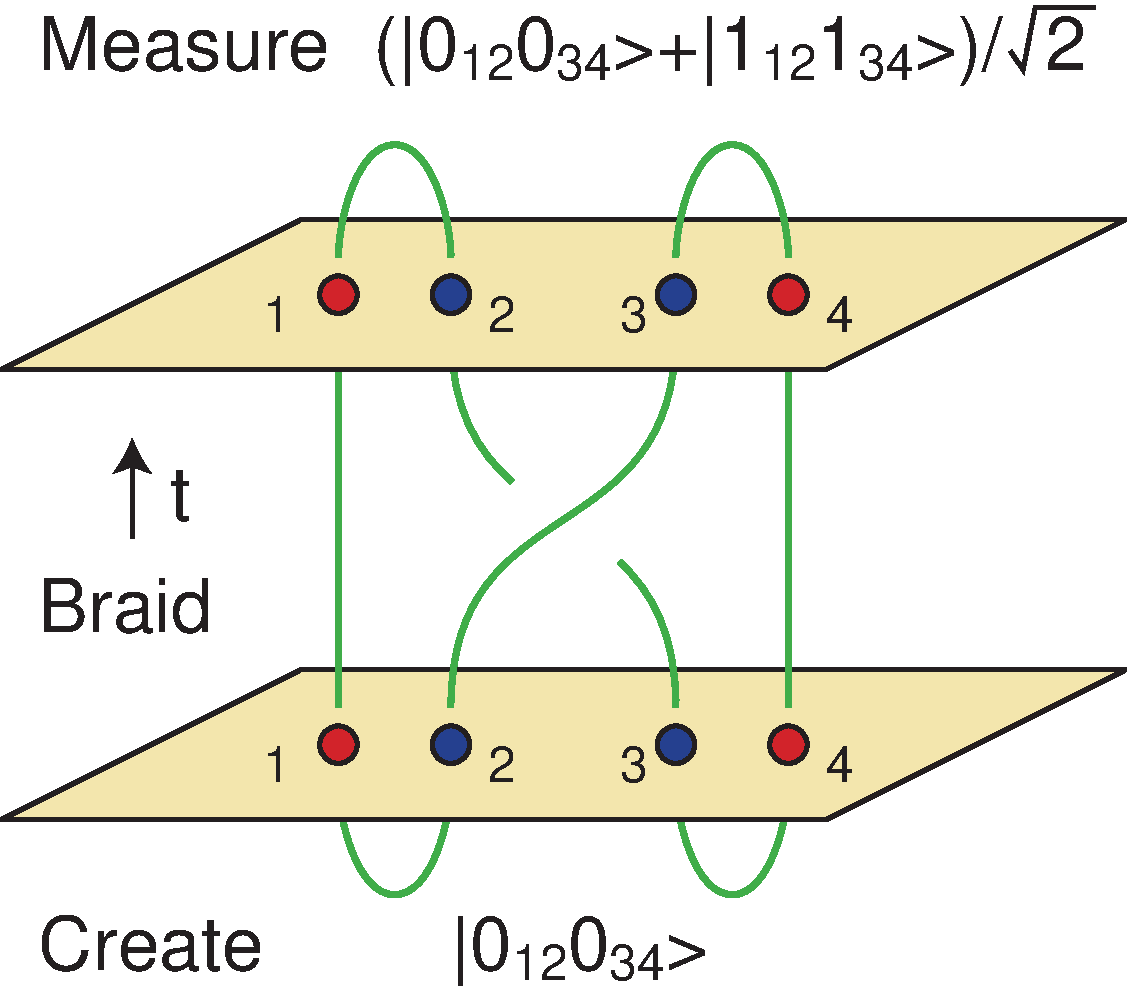
\includegraphics[width=2in]{Fig19}
		\caption{A simple operation in which two vortices are exchanged.  The vortex pairs 12 and 34 are
			created in the vacuum (0 quasiparticle) state.
			When they are brought back together they are in an entangled superposition of
			0 and 1 quasiparticle states.}
		\label{fig:braid}
	\end{figure}
	
	Though the quantum operations allowed by manipulating the Majorana states
	do not have sufficient structure to construct a universal quantum
	computer \cite{freedman02}, the topological protection of the quantum information
	makes the experimental observation of Majorana fermions and non-Abelian
	statistics a high priority in condensed matter
	physics \cite{nayak08}.   Current experimental efforts have focused on the
	$\nu=5/2$ quantum Hall state, where interferometry experiments \cite{sternhalperin06,dassarma05}  can
	in principle detect the non-Abelian statistics predicted for the quasiparticles.
	Though recent experiments on the quantum Hall effect
	have shown encouraging indirect evidence for these states \cite{dolev08,radu08,willett09},
	definitive observation of the Majorana states has remained elusive.
	In the following section we will describe the possibility of
	realizing these states in topological insulator-superconductor
	structures.   The large energy scale associated with the energy gap
	in Bi$_2$Se$_3$ may provide an advantage, so the required temperature
	scale will be limited only by the superconductor.
	
	\subsubsection{Majorana fermions on topological insulators}
	\label{sec:majoranaontopo}
	
	\begin{figure}
		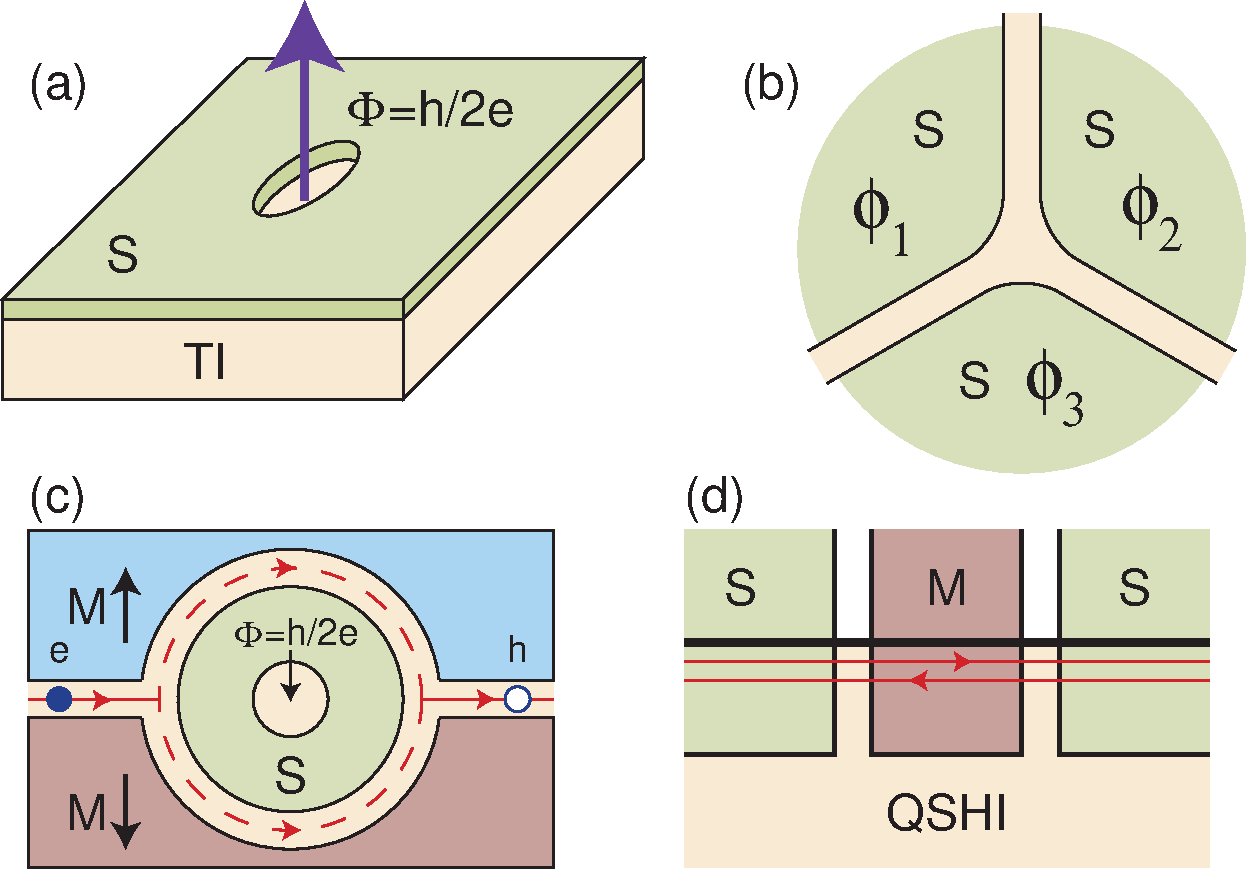
\includegraphics[width=3in]{Fig20}
		\caption{Majorana fermions on topological insulators.  (a) A superconducting vortex, or antidot
			with flux $h/2e$ on a topological insulator is associated with a Majorana zero mode.  (b)
			a superconducting tri-junction on a topological insulator.  Majorana modes
			at the junction can be controlled by adjusting the phases $\phi_{1,2,3}$.  1D chiral
			Majorana modes exist at a superconductor-magnet interface on a topological
			insulator. (c)
			shows a 1D chiral Dirac mode on a magnetic domain wall
			that splits into two chiral Majorana modes around a superconducting island.
			When $\Phi = h/2e$ interference of the Majorana modes converts an electron
			into a hole.  (d) Majorana modes at a superconductor-magnet junction on a 2D QSHI.
		}
		\label{fig:majorana}
	\end{figure}
	
	Consider an interface between a topological insulator and an $s$ wave superconductor.
	Due to the superconducting proximity effect, Cooper pairs may tunnel from the
	superconductor to the surface, leading to
	an induced superconducting energy gap in the surface states.  The resulting
	2D superconducting state is different from an ordinary
	superconductor because the surface states are not spin degenerate and
	contain only half the degrees of freedom of a normal metal.  The
	superconducting state resembles the spinless $p_x+i p_y$ topological superconductor discussed in
	section \ref{sec:superconductor}, which is also based on a spin non degenerate Fermi
	surface.   Unlike the $p_x+i p_y$ superconductor, the surface superconductor does not
	violate ${\cal T}$ symmetry, and its Cooper pairs have even
	parity.  The minus sign required by Fermi statistics is supplied by the $\pi$
	Berry phase of the surface states.  Like the $p_x+ip_y$ superconductor,
	the surface superconductor will have a zero energy Majorana state
	bound to a vortex \cite{fukane08}.
	Similar zero modes were later found for superconducting
	graphene\cite{ghaemi07,bergman09}, though those modes were intrinsically doubled.
	Undoubled Majorana bound states were found earlier by \textcite{jackiw81}
	in a related field theory model that had an extra chiral symmetry.
	Interestingly, the Majorana states on a topological insulator
	emerge as solutions to a 3D BdG theory, so there is a sense in which their
	non-Abelian statistics is inherently three dimensional \cite{teokane10}.
	
	Majorana states can in principle be engineered and manipulated by using junctions of superconductors
	on the surface of a topological insulator \cite{fukane08}.   If the phases on three superconductors
	that meet at a tri-junction (Fig. \ref{fig:majorana}(b)) are arranged such that $(\phi_1,\phi_2,\phi_3) =
	(0,2\pi/3,4\pi/3)$, then a vortex is simulated, and a zero mode will
	be bound to the junction.  If the phases are changed, the zero mode
	can not disappear until the energy gap along one of the three linear
	junctions goes to zero.  This occurs when the phase difference across
	the junction is $\pi$.  At this point the Majorana bound state moves to the
	other end of the linear junction.  Combining these tri-junctions into
	circuits connected by linear junctions could then allow for
	the {\it Create-Braid-Measure} protocol discussed in section
	\ref{sec:qcompute} to be implemented.
	The state of two Majorana modes brought
	together on a linear junction can be probed by measuring the
	supercurrent across that junction.
	
	There are many hurtles to overcome before this ambitious proposal can be realized.
	The first step is finding a suitable superconductor that makes good
	contact with a topological insulator.  Probing the signatures of
	Majorana fermions and non-Abelian statistics will require ingenuity
	-- what makes them good for quantum computing makes them
	hard to measure.  A first step would be to detect the
	Majorana state at a vortex,  antidot or tri-junction by tunneling into
	it from a normal metal.  A signature of the zero mode would
	be a zero bias anomaly, which would have a characteristic
	current-voltage relation \cite{bolech07,law09}.
	
	Another venue for Majorana fermions on a topological insulator surface is a
	linear interface between superconducting and magnetically gapped regions
	\cite{fukane08,tanaka09,linder10}.  This
	leads to a 1D chiral Majorana mode, analogous to the edge state of
	a 2D topological superconductor (Fig. \ref{fig:scedge}(e)).  This can
	be used to construct a novel interferometer for Majorana
	fermions \cite{fukane09b,akhmerov09}.  Fig. \ref{fig:majorana}(c) shows a
	superconducting island surrounded by magnetic regions with a magnetic
	domain wall.  The chiral Dirac fermions on the magnetic domain wall
	incident from the left split into two chiral Majorana fermions on opposite sides of the
	superconductor and then recombine.  If the superconductor encloses a
	flux $\Phi=h/2e$, then the Majorana fermions pick up a relative minus
	sign - analogous to the Aharonov Bohm effect.  This has the effect of
	converting an incident electron into an outgoing hole, with a Cooper
	pair of electrons absorbed by the superconductor.  This could be
	observed in a three terminal transport setup.
	
	Majorana bound states can also be engineered at the edge of a 2D quantum spin Hall insulator
	utilizing magnetic and superconducting energy gaps
	(Fig \ref{fig:majorana}(d)) \cite{fukane09a,nilsson08}.  This and other geometries
	can in principle be used to test the inherent non-locality of Majorana fermion
	states \cite{fu10}
	
	\section{Conclusion and Outlook}
	\label{sec:outlook}
	
	Though the basic properties of topological insulators have been
	established, the field is at an early stage
	in its development.  There is much work to be done to
	realize the potential of these new and fascinating materials.
	In this concluding section we will discuss some very recent
	developments and look toward the future.
	
	In the history of condensed matter physics, the single most important
	ingredient in the emergence of a new field is the perfection of the
	techniques for producing high quality materials.  For example, the
	intricate physics of the fractional quantum Hall effect would never
	have emerged without ultra high mobility GaAs. Topological insulator
	materials need to be perfected, so that they actually insulate. There
	has been substantial progress in this direction.  For instance,
	transport experiments on Ca doped crystals of Bi$_2$Se$_3$ show clear
	insulating behavior below around 100$^\circ$K \cite{checkelsky09}.
	However, the electrical resistance saturates at low temperature,
	and the surface currents appear to be overwhelmed by either bulk
	currents or currents in a layer near the surface.  This is
	a challenging problem because narrow gap semiconductors are very
	sensitive to doping. Nonetheless, it seems clear that there is ample
	room for improvement. Thin films produced, for instance, by
	mechanical exfoliation (as in graphene), or catalytically generated
	Bi$_2$Se$_3$ ribbons and wires \cite{peng09} may be helpful in this
	regard.  A particularly promising new direction is the growth of
	epitaxial films of Bi$_2$Se$_3$
	\cite{zhangg09,zhangy10} and Bi$_2$Te$_3$ \cite{li10}. This has led to the recent observation of Landau
	quantization in the Dirac surface states \cite{cheng10,hanaguri10}. It will be interesting
	to observe such quantization in a transport study.  Present materials pose
	a challenge due to competition between surface and bulk states \cite{taskin09,checkelsky09}.
	The detailed
	study of the electronic and spin transport properties of the surface
	states is called for, complemented by a host of other probes, ranging
	from optics to tunneling spectroscopy.
	
	Another direction for future innovation will be the study of {\it
		heterostructures} involving topological insulators and other
	materials.  In addition to providing a means for protecting and controlling the
	population of the surface states, such structures could provide a step towards the
	longer term goal of engineering exotic states, such as Majorana
	fermions, with the surface states.  There are many materials problems
	to be solved in order to find appropriate magnetic and
	superconducting materials which exhibit the appropriate proximity
	effects with the surface states, and detailed experiments will be
	necessary to characterize those states.  An exciting recent development
	along these lines is the discovery of superconductivity in Cu doped
	Bi$_2$Se$_3$ \cite{hor10a}.  One can imagine devices fabricated
	with techniques of {\it modulation doping} that have proved extremely
	powerful in semiconductor physics.  One can also imagine other devices that
	integrate magnetic materials with topological insulators, to take advantage of
	the special spin properties of the surface states.
	
	Topological insulating behavior is likely to arise in other classes
	of materials, in addition to the binary compounds Bi$_{1-x}$Sb$_x$,
	Bi$_2$Te$_3$, Bi$_2$Se$_3$ and Sb$_2$Te$_3$.
	If one expands ones horizon to ternary compounds (or beyond) the
	possibilities for exotic materials multiply.  Candidate materials will be narrow
	gap semiconductors which include heavy elements.  One intriguing class
	of materials are transition metal oxides involving iridium.
	\textcite{shitade09} have predicted that
	Na$_2$IrO$_3$ is a weak topological insulator.  \textcite{pesin10}
	have suggested that certain iridium based pyrochlore compounds
	%such as Pr$_2$Ir$_2$O$_7$
	may be strong topological insulators.  Since these materials
	involve $d$ electrons, a crucial issue will be to understand the interplay
	between strong electron-electron interactions and the spin-orbit interaction.
	Very recent theoretical work predicts topological insulator behavior
	in ternary Heusler compounds\cite{lin10a,chadov10} and other materials
	\cite{lin10b,lin10c,yan10}.
	These are exciting new directions where further theoretical and experimental
	work is called for.
	
	Topological superconductors present another exciting frontier direction.
	In addition to observing the surface Majorana modes predicted for $^3$He B \cite{chung09}, it will be very
	interesting to predict and observe electronic topological superconductors,
	to characterize their surface modes
	and to explore their potential utility.  To this end there
	has been recent progress in developing methods to theoretically identify topological
	superconductors based on their band structure \cite{qi10,fuberg10}.
	
	More generally there may be other interesting correlated states related to topological
	insulators and superconductors.  For example, \textcite{levin09} showed that
	a ${\cal T}$ invariant {\it fractional} quantum spin Hall state can be topologically stable.
	This points to a general theoretical problem associated with the
	topological classification of {\it interacting} systems: How do we
	unify the seemingly different notions of topological order
	epitomized by \textcite{thouless82} and by \textcite{wen95}?
	The topological field theories studied by
	\textcite{qihugheszhang08}, as well as tantalizing connections
	with string theory \cite{ryu10} provide steps in this direction, but a complete
	theory remains to be developed.
	
	To conclude, the recent advances in the physics of topological insulators have been driven
	by a rich interplay between theoretical insight and experimental
	discoveries.  There is reason for optimism that this field
	will continue to develop in exciting new directions.
	
	\section*{Acknowledgments} C.L.K. thanks E. J. Mele, L. Fu and
	J. C. Y. Teo for collaboration and NSF Grant DMR 0906175 for support.
	M.Z.H. thanks L. A. Wray for assistance preparing figures and
	A. Bansil, R. J. Cava, J. G. Checkelsky, J. H. Dil, A.
	V. Fedorov, Y. S. Hor, D. Hsieh, H. Lin, F. Meier, N. P. Ong, J.
	Osterwalder, L. Patthey, D. Qian, P. Roushan, L. A. Wray, Y. Xia and A. Yazdani  for
	collaborations and U.S. DOE (Grants No. DE-FG-02-05ER46200, No. AC03-76SF00098, and No. DE-FG02-
	07ER46352), NSF [Grant No. DMR-0819860 (materials)
	DMR-1006492], Alfred P. Sloan Foundation, and Princeton
	University for support.
	
	
	
	\bibliographystyle{apsrmp}
	\begin{thebibliography}{99}
		
		\bibitem[Agergaard, \emph{et al.}(2001)]{agergaard01}
		%Agergaard, S., \emph{et al.}, 2001,
		Agergaard, S., C. Sondergaard, H. Li, M. B. Nielsen, S. V. Hoffmann,
		Z. Li and Ph. Hofmann, 2001,
		New J. Phys. {\bf 3}, 15.
		
		\bibitem[Akhmerov, Nilsson and Beenakker(2009)]{akhmerov09}
		Akhmerov, A. R., J. Nilsson, and C. W. J. Beenakker, 2009,
		Phys. Rev. Lett. {\bf 102}, 216404.
		
		\bibitem[Alpichshev, \emph{et al.}(2010)]{alpichshev10}
		Alpichshev, Z., J. G. Analytis, J. H. Chu, I. R. Fisher, Y. L. Chen, Z. X. Shen,
		A. Fang, and A. Kapitulnik, 2010,
		Phys. Rev. Lett. {\bf 104}, 016401.
		
		\bibitem[Altland and Zirnbauer(1997)]{altland97}
		Altland, A., and M. R. Zirnbauer, 1997,
		Phys. Rev. B {\bf 55}, 1142.
		
		\bibitem[Anderson(1958)]{anderson58}
		Anderson, P. W., 1958,
		Phys. Rev. {\bf 109}, 1492.
		
		\bibitem[Ast and H\"ochst(2001)]{ast01}
		Ast, C. R.  and H. H\"ochst, 2001,
		Phys. Rev. Lett. {\bf 87}, 177602.
		
		\bibitem[Avignone, Elliott and Engel(2008)]{avignone08}
		Avignone, F. T., S. R. Elliott, and J. Engel, 2008,
		Rev. Mod. Phys. {\bf 80}, 481.
		
		\bibitem[Bergman and Le Hur(2009)]{bergman09}
		Bergman, D. L. and K. Le Hur, 2009,
		Phys. Rev. B {\bf 79}, 184520.
		
		\bibitem[Bernevig, Hughes and Zhang(2006)]{bernevighugheszhang06}
		Bernevig, B. A., T. A. Hughes, and S. C. Zhang, 2006,
		Science {\bf 314}, 1757.
		
		\bibitem[Bernevig and Zhang(2006)]{bernevig06}
		Bernevig, B. A. and S. C. Zhang, 2006,
		Phys. Rev. Lett. {\bf 96}, 106802.
		
		\bibitem[Berry(1984)]{berry84}
		Berry, M. V., 1984,
		Proc. R. Soc. Lond. A {\bf 392}, 45.
		
		\bibitem[Bloch(1929)]{bloch29}
		Bloch, F., 1929,
		Z. Physik {\bf 52}, 555.
		
		\bibitem[Boettger and Trickey(2007)]{boettger07}
		Boettger, J. C., and S. B. Trickey, 2007,
		Phys. Rev. B {\bf 75}, 121402(R).
		
		\bibitem[Bolech and Demler(2007)]{bolech07}
		Bolech, C. J. and E. Demler, 2007,
		Phys. Rev. Lett. {\bf 98}, 237002.
		
		\bibitem[Bonderson, Freedman and Nayak(2008)]{bonderson08}
		Bonderson P., M. Freedman and C. Nayak, 2008,
		Phys. Rev. Lett. {\bf 101}, 010501.
		
		\bibitem[B\"uttiker(1988)]{buttiker88}
		B\"uttiker, M., 1988,
		Phys. Rev. B {\bf 38}, 9375.
		
		\bibitem[Cade(1985)]{cade85}
		Cade, N. A., 1985,
		J. Phys. C {\bf 18}, 5135.
		
		\bibitem[Caroli, de Gennes and Matricon(1964)]{caroli64}
		Caroli, C., P. G. de Gennes and J. Matricon, 1964,
		Phys. Lett. {\bf 9}, 307.
		
		\bibitem[Castro Neto, \emph{et al.}(2009)]{neto09}
		Castro Neto, A. H., F. Guinea, N. M. R. Peres, K. S. Novoselov and A. K. Geim, 2009,
		Rev. Mod. Phys. {\bf 81}, 109.
		
		\bibitem[Chadov, \emph{et al.}(2010)]{chadov10}
		Chadov, S., X. L. Qi, J K\"ubler, G. H. Fecher, C. Felser, S. C. Zhang, 2010,
		Nature Materials {\bf 9}, 541.
		
		\bibitem[Chang, \emph{et al.}(1985)]{chang85}
		Chang, Y. C., J. N. Schulman, G. Bastard, Y. Guldner and M. Voos, 1985,
		Phys. Rev. B {\bf 31}, 2557.
		
		
		\bibitem[Checkelsky, \emph{et al.}(2009)]{checkelsky09}
		%Checkelsky, J. G., \emph{et al.}, 2009,
		Checkelsky, J. G., Y. S. Hor, M. H. Liu, D. X. Qu, R. J. Cava, and N. P. Ong, 2009,
		Phys. Rev. Lett. {\bf 103}, 246601.
		
		\bibitem[Chen, \emph{et al.}(2009)]{chen09}
		Chen, Y. L., J. G. Analytis, J. H. Chu, Z. K. Liu, S. K. Mo, X. L. Qi, H. J. Zhang,
		D. H. Lu, X. Dai, Z. Fang, S. C. Zhang, I. R. Fisher, Z. Hussain, Z. X. Shen, 2009,
		Science {\bf 325}, 178.
		
		\bibitem[Cheng, \emph{et al.}(2010)]{cheng10}
		%Cheng P., \emph{et al.}, 2010,
		Cheng P., C. Song, T. Zhang, Y. Zhang, Y. Wang, J. F. Jia, J. Wang, Y. Wang, B. F. Zhu,
		X. Chen, X. Ma, K. He, L. Wang, X. Dai, Z. Fang, X. C. Xie, X. L. Qi, C. X. Liu,
		S. C. Zhang and Q. K. Xue, 2010,
		Phys. Rev. Lett. {\bf 105}, 076801 (2010).
		
		\bibitem[Chung and Zhang(2009)]{chung09}
		Chung, S. B. and S. C. Zhang, 2009,
		Phys. Rev. Lett. {\bf 103}, 235301.
		
		\bibitem[Das Sarma, Freedman and Nayak(2005)]{dassarma05}
		Das Sarma, S., M. Freedman, and C. Nayak, 2005,
		Phys. Rev. Lett. {\bf 94}, 166802.
		
		\bibitem[Das Sarma, Nayak and Tewari(2006)]{dassarma06}
		Das Sarma, S., C. Nayak, and S. Tewari, 2006,
		Phys. Rev. B {\bf 73}, 220502(R).
		
		\bibitem[De Gennes(1966)]{degennes66}
		De Gennes, P. G., 1966,
		{\it Superconductivity of Metals and Alloys} (W. A. Benjamin, New York).
		
		\bibitem[DiVincenzo and Mele(1984)]{divencenzo84}
		DiVincenzo, D. P. and E. J. Mele, 1984,
		Phys. Rev. B {\bf 29}, 1685.
		
		\bibitem[Dolev, \emph{et al.}(2008)]{dolev08}
		Dolev, M., M. Heiblum, V. Umansky, A. Stern, and D. Mahalu, 2008,
		Nature {\bf 452}, 829.
		
		\bibitem[Dornhaus and Nimtz(1983)]{dornhaus83}
		Dornhaus R. and G. Nimtz, 1983,
		{\it Narrow Gap Semiconductors},
		Springer Tracts in Modern Physics {\bf 98} (Springer, Berlin).
		
		\bibitem[Essin, Moore and Vanderbilt(2009)]{essin09}
		Essin, A. M., J. E. Moore and D. Vanderbilt, 2009,
		Phys. Rev. Lett. {\bf 102}, 146805.
		
		\bibitem[Fradkin, Dagotto and Boyanovsky(1986)]{fradkin86}
		Fradkin E., E. Dagotto, and D. Boyanovsky, 1986, Phys. Rev.
		Lett. {\bf 57}, 2967.
		
		\bibitem[Freedman, Larsen and Wang(2002)]{freedman02}
		Freedman, M. H., M. Larsen, and Z. Wang, 2002,
		Commun. Math. Phys. {\bf 227}, 605.
		
		\bibitem[Fu(2009)]{fu09}
		Fu, L., 2009,
		Phys. Rev. Lett. {\bf 103}, 266801.
		
		\bibitem[Fu(2010)]{fu10}
		Fu, L., 2010,
		Phys. Rev. Lett. {\bf 104}, 056402.
		
		\bibitem[Fu and Berg(2009)]{fuberg10}
		Fu, L., and E. Berg, 2009,
		Phys. Rev. Lett. {\bf 105}, 097001 (2010).
		
		\bibitem[Fu and Kane(2006)]{fukane06}
		Fu, L. and C. L. Kane, 2006,
		Phys.\ Rev.\ B\ {\bf 74}, 195312.
		
		\bibitem[Fu and Kane(2007)]{fukane07}
		Fu, L. and C. L. Kane, 2007,
		Phys. Rev. B {\bf 76}, 045302.
		
		\bibitem[Fu and Kane(2008)]{fukane08}
		Fu, L. and C. L. Kane, 2008,
		Phys. Rev. Lett. {\bf 100}, 096407.
		
		\bibitem[Fu and Kane(2009a)]{fukane09a}
		Fu, L. and C. L. Kane, 2009,
		Phys. Rev. B {\bf 79}, 161408(R).
		
		\bibitem[Fu and Kane(2009b)]{fukane09b}
		Fu, L. and C. L. Kane, 2009,
		Phys. Rev. Lett. {\bf 102}, 216403.
		
		\bibitem[Fu, Kane and Mele(2007)]{fukanemele07}
		Fu, L., C. L. Kane and E. J. Mele, 2007,
		Phys. Rev. Lett. {\bf 98}, 106803.
		
		\bibitem[Fukui, Fujiwara and Hatsugai(2008)]{fukui08}
		Fukui, T., T. Fujiwara and Y. Hatsugai, 2008,
		J. Phys. Soc. Jpn. {\bf 77} 123705.
		
		\bibitem[Fukui and Hatsugai(2007)]{fukui07}
		Fukui, T. and Y. Hatsugai, 2007,
		J. Phys. Soc. Jpn. {\bf 76}, 053702.
		
		\bibitem[Geim and Novoselov(2007)]{geim07}
		Geim A. V. and K. S. Novoselov, 2007,
		Nature Mater. {\bf 6}, 183.
		
		\bibitem[Ghaemi and Wilczek(2007)]{ghaemi07}
		Ghaemi P. and F. Wilczek, 2007,
		arXiv:0709.2626 (unpublished).
		
		\bibitem[Gmitra, \emph{et al.}(2009)]{gmitra09}
		%Gmitra, M., \emph{et al.}, 2009,
		Gmitra, M., S. Konschuh, C. Ertler, C. Ambrosch-Draxl, and J. Fabian, 2009,
		Phys. Rev. B {\bf 80}, 235431.
		
		\bibitem[Greiter, Wen and Wilczek(1992)]{greiter92}
		Greiter, M., X. G. Wen, and F. Wilczek, 1992,
		Nucl. Phys. B {\bf 374}, 567.
		
		\bibitem[Guo and Franz(2009)]{guo09}
		Guo, H. M. and M. Franz, 2009,
		Phys. Rev. Lett. {\bf 103}, 206805.
		
		\bibitem[Gurarie, Radzihovsky and Andreev(2005)]{gurarie05}
		Gurarie, V., L. Radzihovsky, and A. V. Andreev, 2005,
		Phys. Rev. Lett. {\bf 94}, 230403.
		
		\bibitem[Haldane(1988)]{haldane88}
		Haldane, F. D. M., 1988,
		Phys. Rev. Lett. {\bf 61}, 2015.
		
		\bibitem[Halperin(1982)]{halperin82}
		Halperin, B. I., 1982,
		Phys. Rev. B {\bf 25}, 2185.
		
		\bibitem[Hanaguri, \emph{et al.}(2010)]{hanaguri10}
		Hanaguri, T., K. Igarashi, M. Kawamura, H. Takagi, T. Sasagawa, 2010,
		Phys. Rev. B {\bf 82}, 081305(R) (2010).
		
		\bibitem[Hasan, Lin and Bansil(2009)]{hasan09}
		Hasan, M. Z., H. Lin, A. Bansil, 2009,
		Physics {\bf 2}, 108.
		
		\bibitem[Hirahara, \emph{et al.}(2006)]{hirahara06}
		%Hirahara, T., \emph{et al.}, 2006
		Hirahara, T, T. Nagao, I. Matsuda, G. Bihlmayer, E. V. Chulkov,
		Y. M. Koroteev, P. M. Echenique, M. Saito, and S. Hasegawa, 2006
		Phys. Rev. Lett. {\bf 97}, 146803.
		
		\bibitem[Hofmann(2006)]{hofmann06}
		Hofmann, Ph., 2006,
		Prog. Surf. Sci. {\bf 81}, 191.
		
		\bibitem[Hor, \emph{et al.}(2009)]{hor09}
		Hor, Y. S., A. Richardella, P. Roushan, Y. Xia, J. G. Checkelsky, A. Yazdani,
		M. Z. Hasan, N. P. Ong, and R. J. Cava, 2009,
		Phys. Rev. B {\bf 79}, 195208.
		
		\bibitem[Hor, \emph{et al.}(2010a)]{hor10a}
		%Hor, Y. S., \emph{et al.}, 2010a,
		Hor, Y. S., A. J. Williams, J. G. Checkelsky, P. Roushan, J. Seo, Q. Xu, H. W. Zandbergen,
		A. Yazdani, N. P. Ong, R. J. Cava, 2010a,
		Phys. Rev. Lett. {\bf 104}, 057001.
		
		\bibitem[Hor, \emph{et al.}(2010b)]{hor10b}
		Hor, Y. S., P. Roushan, H. Beidenkopf, J. Seo, D. Qu, J. G. Checkelsky,
		L. A. Wray, Y. Xia, S.-Y. Xu, D. Qian, M. Z. Hasan, N. P. Ong,
		A. Yazdani, R. J. Cava, 2010b,
		Phys. Rev. B {\bf 81}, 195203 (2010).
		
		\bibitem[Hsieh, \emph{et al.}(2008)]{hsieh08}
		%Hsieh D., \emph{et al.}, 2008,
		Hsieh, D., D. Qian, L. Wray, Y. Xia, Y. S. Hor, R. J. Cava and M. Z. Hasan, 2008,
		Nature {\bf 452}, 970.
		
		\bibitem[Hsieh, \emph{et al.}(2009a)]{hsieh09a}
		Hsieh, D., Y. Xia, L. Wray, D. Qian, A. Pal, J. H. Dil, J. Osterwalder, F. Meier, G. Bihlmayer,
		C. L. Kane, Y. S. Hor, R. J. Cava and M. Z. Hasan, 2009a,
		Science {\bf 323}, 919.
		
		\bibitem[Hsieh, \emph{et al.}(2009b)]{hsieh09b}
		Hsieh, D., Y. Xia, D. Qian, L. Wray, J. H. Dil, F. Meier, J. Osterwalder, L. Patthey,
		J. G. Checkelsky, N. P. Ong, A. V. Fedorov, H. Lin, A. Bansil, D. Grauer, Y. S. Hor,
		R. J. Cava and M. Z. Hasan, 2009b,
		Nature {\bf 460}, 1101.
		
		\bibitem[Hsieh, \emph{et al.}(2009c)]{hsieh09c}
		Hsieh, D., Y. Xia, D. Qian, L. Wray, F. Meier, J. H. Dil, J. Osterwalder, L. Patthey,
		A. V. Fedorov, H. Lin, A. Bansil, D. Grauer, Y. S. Hor, R. J. Cava, and M. Z. Hasan, 2009c,
		Phys. Rev. Lett. {\bf 103}, 146401.
		
		\bibitem[Hsieh, \emph{et al.}(2009d)]{hsieh09d}
		Hsieh, D., Y. Xia, L. Wray, D. Qian, A. Pal, J. H. Dil, F. Meier, J. Osterwalder,
		G. Bihlmayer, C. L. Kane, Y. S. Hor, R. J. Cava and M. Z. Hasan, 2009d,
		arXiv:0909.5509.
		
		\bibitem[Hsieh, \emph{et al.}(2010)]{hsieh10}
		Hsieh, D., Y. Xia, L. Wray, D. Qian, A. Pal, J. H. Dil, F. Meier, J. Osterwalder,
		G. Bihlmayer, C. L. Kane, Y. S. Hor, R. J. Cava, M. Z. Hasan, 2010,
		arXiv:1001.1574.
		
		\bibitem[Huertas-Hernando, Guinea and Brataas(2006)]{huertas06}
		Huertas-Hernando, D.,  F. Guinea, and A. Brataas, 2006,
		Phys. Rev. B {\bf 74}, 155426.
		
		\bibitem[Ivanov(2001)]{ivanov01}
		Ivanov, D. A., 2001,
		Phys. Rev. Lett. {\bf 86}, 268.
		
		\bibitem[Jackiw(1984)]{jackiw84}
		Jackiw, R., 1984,
		Phys. Rev. D {\bf 29}, 2375.
		
		\bibitem[Jackiw and Rebbi(1976)]{jackiw76}
		Jackiw, R. and C. Rebbi, 1976
		Phys. Rev. D {\bf 13}, 3398.
		
		\bibitem[Jackiw and Rossi(1981)]{jackiw81}
		Jackiw, R. and P. Rossi, 1981,
		Nucl. Phys. B, {\bf 190} 681.
		
		\bibitem[Kane and Mele(2005a)]{kanemele05a}
		Kane, C. L. and E. J. Mele, 2005a,
		Phys. Rev. Lett. {\bf 95}, 226801.
		
		\bibitem[Kane and Mele(2005b)]{kanemele05b}
		Kane, C. L. and E. J. Mele, 2005b,
		Phys. Rev. Lett. {\bf 95}, 146802.
		
		\bibitem[Kaplan(1992)]{kaplan92}
		Kaplan, D. B., 1992,
		Phys. Lett. B {\bf 288} 342.
		
		\bibitem[Kitaev(2000)]{kitaev00}
		Kitaev, A., 2000,
		arXiv:cond-mat/0010440 (unpublished).
		
		\bibitem[Kitaev(2003)]{kitaev03}
		Kitaev, A., 2003,
		Ann. Phys. {\bf 303}, 2.
		
		\bibitem[Kitaev(2009)]{kitaev09}
		Kitaev, A., 2009,
		AIP Conf. Proc. {\bf 1134}, 22.
		
		\bibitem[Kohmoto, Halperin and Wu(1992)]{kohmoto92}
		Kohmoto, M., B. I. Halperin, and Y. S. Wu, 1992,
		Phys. Rev. B {\bf 45}, 13488.
		
		\bibitem[K\"onig, \emph{et al.}(2007)]{konig07}
		%K\"onig, M., \emph{et al.}, 2007,
		K\"onig, M., S. Wiedmann, C. Br�ne, A. Roth, H. Buhmann, L. W. Molenkamp,
		X. L. Qi and S. C. Zhang, 2007,
		Science {\bf 318}, 766.
		
		\bibitem[K\"onig, \emph{et al.}(2008)]{konig08}
		%K\"onig M., \emph{et al.}, 2008,
		K\"onig, M., H. Buhmann, L. W. Molenkamp, T. Hughes, C. X. Liu,
		X. L. Qi and S. C. Zhang, 2008,
		J. Phys. Soc. Jpn. {\bf 77}, 031007.
		
		\bibitem[Laughlin(1983)]{laughlin83}
		Laughlin, R. B., 1983,
		Phys. Rev. Lett. {\bf 50}, 1395.
		
		\bibitem[Law, Lee and Ng(2009)]{law09}
		Law, K. T., P. A. Lee, and T. K. Ng, 2009,
		Phys. Rev. Lett. {\bf 103}, 237001.
		
		\bibitem[Lee(2009)]{lee09}
		Lee, P. A., 2009,
		arXiv:0907.2681 (unpublished).
		
		\bibitem[Lee and Ramakrishnan(1985)]{lee85}
		Lee, P. A.  and T. V. Ramakrishnan, 1985,
		Rev. Mod. Phys. {\bf 57}, 287.
		
		\bibitem[Lenoir, \emph{et al.}(1996)]{lenoir96}
		Lenoir, B., A. Dauscher, X. Devaux, R. Martin-Lopez, Y. I. Ravich,
		H. Scherrer and S Scherrer, 1996, in
		{\it Fifteenth International Conference on Thermoelectrics}
		(IEEE, New York) p. 1-13.
		
		\bibitem[Levin and Stern(2009)]{levin09}
		Levin, M. and A. Stern, 2009,
		Phys. Rev. Lett. {\bf 103}, 196803.
		
		\bibitem[Li, \emph{et al.}(2009)]{li10}
		%Li, Y. Y., \emph{et al.}, 2009,
		Li, Y. Y., G. Wang, X. G.  Zhu, M. H. Liu, C. Ye, X. Chen, Y. Y. Wang,
		K. He, L. L. Wang, X. C. Ma, H. J. Zhang, X. Dai, Z. Fang, X. C. Xie,
		Y. Liu, X. L. Qi, J. F. Jia, S. C. Zhang, Q. K. Xue, 2009,
		arXiv:0912.5054.
		
		\bibitem[Lin, \emph{et al.}(2010a)]{lin10a}
		Lin, H., L. A. Wray, Y. Xia, S. Jia, R. J. Cava, A. Bansil, M. Z. Hasan, 2010,
		Nature Materials {\bf 9}, 546.
		
		\bibitem[Lin, \emph{et al.}(2010b)]{lin10b}
		Lin, H., L. A. Wray, Y. Xia, S. Y. Xu, S. Jia, R. J. Cava, A. Bansil, M. Z. Hasan, 2010,
		arXiv:1003.2615.
		
		\bibitem[Lin, \emph{et al.}(2010c)]{lin10c}
		Lin, H., R. S. Markiewicz, L. A. Wray, L. Fu, M. Z. Hasan, and A. Bansil, 2010,
		Phys. Rev. Lett. {\bf 105}, 036404.
		
		\bibitem[Lin-Liu and Sham(1985)]{linliu85}
		Lin-Liu, Y. R. and L. J. Sham, 1985,
		Phys. Rev. B {\bf 32}, 5561.
		
		\bibitem[Linder, \emph{et al.}(2010)]{linder10}
		Linder, J., Y. Tanaka, T. Yokoyama, A. Sudbo and N. Nagaosa, 2010,
		Phys. Rev. Lett. {\bf 104}, 067001.
		
		\bibitem[Liu and Allen(1995)]{liuallen95}
		Liu, Y. and R. E. Allen, 1995,
		Phys. Rev. B {\bf 52}, 1566.
		
		\bibitem[Maciejko, \emph{et al.}(2009)]{maciejko09}
		%Maciejko, J., \emph{et al.}, 2009,
		Maciejko, J., C. Liu, Y. Oreg, X. L. Qi, C. Wu, S. C. Zhang, 2009,
		Phys. Rev. Lett. {\bf 102}, 256803.
		
		\bibitem[Majorana(1937)]{majorana37}
		Majorana, E., 1937,
		Nuovo Cimento {\bf 5}, 171.
		
		\bibitem[Min, \emph{et al.}(2006)]{min06}
		%Min, H., \emph{et al.}, 2006,
		Min, H., J. E. Hill, N. A. Sinitsyn, B. R. Sahu, L. Kleinman and A. H.
		MacDonald, 2006,
		Phys. Rev. B {\bf 74}, 165310.
		
		\bibitem[Moore and Read(1991)]{mooreread91}
		Moore, G. and N. Read, 1991,
		Nucl. Phys. B {\bf 360}, 362.
		
		\bibitem[Moore(2009)]{moore09}
		Moore, J. E., 2009,
		Nature Phys. {\bf 5}, 378.
		
		\bibitem[Moore(2010)]{moore10}
		Moore, J. E., 2010, Nature {\bf 464}, 194.
		
		\bibitem[Moore and Balents(2007)]{moorebalents07}
		Moore, J. E. and L. Balents, 2007,
		Phys. Rev. B {\bf 75}, 121306(R).
		
		\bibitem[Murakami, Nagaosa and Zhang(2004)]{murakami04}
		Murakami, S., N. Nagaosa, and S. C. Zhang, 2004,
		Phys. Rev. Lett. {\bf 93}, 156804.
		
		\bibitem[Nagato, Higashitani and Nagai(2009)]{nagato09}
		Nagato, Y., S. Higashitani and K. Nagai, 2009,
		J. Phys. Soc. Jpn. {\bf 78}, 123603.
		
		\bibitem[Nakahara(1990)]{nakahara90}
		Nakahara, M., 1990,
		{\it Geometry, Topology and Physics} (Adam Hilger, Bristol).
		
		\bibitem[Nayak, \emph{et al.}(2008)]{nayak08}
		Nayak, C., S. H. Simon, A. Stern, M. Freedman, and S. Das Sarma, 2008,
		Rev. Mod. Phys. {\bf 80}, 1083.
		
		\bibitem[Nayak and Wilczek(1996)]{nayak96}
		Nayak C., and F. Wilczek, 1996,
		Nucl. Phys. B {\bf 479}, 529.
		
		\bibitem[Nielssen and Ninomiya(1983)]{nielssen83}
		Nielssen, H. and N. Ninomiya, 1983,
		Phys. Lett. 130B, 389.
		
		\bibitem[Nilsson, Akhmerov and Beenakker(2008)]{nilsson08}
		Nilsson J., A. R. Akhmerov, and C. W. J. Beenakker, 2008
		Phys. Rev. Lett. {\bf 101}, 120403.
		
		\bibitem[Nishide, \emph{et al.}(2010)]{nishide10}
		Nishide, A., A. A. Taskin, Y. Takeichi, T. Okuda, A. Kakizaki, T. Hirahara,
		K. Nakatsuji, F. Komori, Y. Ando and I. Matsuda, 2010,
		Phys. Rev. B {\bf 81}, 041309(R).
		
		\bibitem[Noh, \emph{et al.}(2008)]{noh08}
		Noh, H. J., H. Koh, S. J. Oh, J. H. Park, H. D. Kim, J. D. Rameau, T. Valla,
		T. E. Kidd, P. D. Johnson, Y. Hu and Q. Li, 2008,
		Europhys. Lett. {\bf 81}, 57006.
		
		\bibitem[Nomura, Koshino and Ryu(2007)]{nomura07}
		Nomura K., M. Koshino, S. Ryu, 2007,
		Phys. Rev. Lett. {\bf 99}, 146806.
		
		\bibitem[Novoselov, \emph{et al.}(2005)]{novoselov05}
		%Novoselov, K. S., \emph{et al.}, 2005,
		Novoselov, K. S., A. K. Geim, S. V. Morozov, D. Jiang, M. I. Katsnelson,
		I. V. Grigorieva, S. V. Dubonos and A. A. Firsov, 2005,
		Nature {\bf 438}, 197.
		
		\bibitem[Pankratov(1987)]{pankratov87}
		Pankratov, O. A., 1987,
		Phys. Lett. A {\bf 121}, 360.
		
		\bibitem[Pankratov, Pakhomov and Volkov(1987)]{pankratovpakhomov87}
		Pankratov, O. A., S. V. Pakhomov and B. A. Volkov, 1987,
		Solid State Comm. {\bf 61}, 93.
		
		\bibitem[Park, \emph{et al.}(2010)]{park10}
		Park, S. R., W. S. Jung, C. Kim, D. J. Song, C. Kim, S. Kimura, K. D. Lee and N. Hur, 2010,
		Phys. Rev. B {\bf 81}, 041405(R).
		
		\bibitem[Patthey, Schneider and Micklitz(1994)]{patthey94}
		Patthey, F., W. D. Schneider, and H. Micklitz, 1994,
		Phys. Rev. B {\bf 49}, 11293.
		
		\bibitem[Peng, \emph{et al.}(2010)]{peng09}
		%Peng H., \emph{et al.}, 2009,
		Peng, H., K. Lai, D. Kong, S. Meister, Y. Chen, X. L. Qi, S. C. Zhang, Z. X. Shen, Y. Cui, 2010,
		Nature Materials {\bf 9}, 225.
		
		\bibitem[Pesin and Balents(2010)]{pesin10}
		Pesin, D. A. and L. Balents, 2010,
		Nat. Phys. {\bf 6}, 376.
		
		\bibitem[Prange and Girvin(1987)]{prange87}
		Prange, R. E. and S. M. Girvin, 1987,
		{\it The Quantum Hall Effect} (Springer, New York).
		
		\bibitem[Qi, Hughes and Zhang(2008)]{qihugheszhang08}
		Qi, X. L., T. L. Hughes, and S. C. Zhang, 2008,
		Phys. Rev. B {\bf 78}, 195424.
		
		\bibitem[Qi, Hughes and Zhang(2010)]{qi10}
		Qi, X. L., T. L. Hughes, and S. C. Zhang, 2010,
		Phys. Rev. B {\bf 81}, 134508.
		
		\bibitem[Qi, \emph{et al.}(2009)]{qihughesraduzhang09}
		Qi, X. L., T. L. Hughes, S. Raghu and S. C. Zhang, 2009,
		Phys. Rev. Lett. {\bf 102}, 187001.
		
		\bibitem[Qi, Wu and Zhang(2006)]{qi06}
		Qi, X. L., Y. S. Wu and S. C. Zhang, 2006,
		Phys. Rev. B {\bf 74}, 085308.
		
		\bibitem[Qi, \emph{et al.}(2009)]{qizhang09}
		Qi, X. L., R. Li, J. Zang and S. C. Zhang, 2009,
		Science {\bf 323}, 1184.
		
		\bibitem[Qi and Zhang(2010)]{qizhang10}
		Qi, X. L. and S. C. Zhang, 2010,
		Physics Today, {\bf 63}, 33.
		
		\bibitem[Radu, \emph{et al.}(2008)]{radu08}
		Radu, P., J. B. Miller, C. M. Marcus, M. A. Kastner, L. N. Pfeiffer and K. W. West, 2008,
		Science {\bf 320}, 899.
		
		\bibitem[Ran, Zhang and Vishwanath(2009)]{ran09}
		Ran, Y., Y. Zhang and A. Vishwanath, 2009,
		Nat. Phys. {\bf 5}, 298.
		
		\bibitem[Read and Green(2000)]{readgreen00}
		Read, N. and D. Green, 2000,
		Phys. Rev. B {\bf 61}, 10267.
		
		\bibitem[Roth, \emph{et al.}(2009)]{roth09}
		Roth A., C. Br\"une, H. Buhmann, L. W. Molenkamp, J. Maciejko, X. L. Qi, and S. C. Zhang, 2009,
		Science {\bf 325}, 294.
		
		\bibitem[Roushan, \emph{et al.}(2009)]{roushan09}
		Roushan, P., J. Seo, C. V. Parker, Y. S. Hor, D. Hsieh, D. Qian, A. Richardella, M. Z. Hasan,
		R. J. Cava and A. Yazdani, 2009,
		Nature {\bf 460}, 1106.
		
		\bibitem[Roy(2008)]{roy08}
		Roy, R., 2008,
		arXiv:0803.2868 (unpublished).
		
		\bibitem[Roy(2009a)]{roy09a}
		Roy, R., 2009,
		Phys. Rev. B {\bf 79}, 195321; arXiv:cond-mat/0604211.
		
		\bibitem[Roy(2009b)]{roy09b}
		Roy, R., 2009,
		Phys. Rev. B {\bf 79}, 195322; arXiv:cond-mat/0607531.
		
		\bibitem[Ryu, \emph{et al.}(2010)]{ryu09}
		Ryu, S., A. Schnyder, A. Furusaki, A. W. W.  Ludwig, 2010,
		New J. Phys. {\bf 12}, 065010.
		
		\bibitem[Ryu and Takayanagi(2010)]{ryu10}
		Ryu, S. and T. Takayanagi, 2010,
		arXiv:1001.0763.
		
		\bibitem[Sato and Fujimoto(2009)]{sato09}
		Sato, M. and S. Fujimoto, 2009,
		Phys. Rev. B {\bf 79}, 094504.
		
		\bibitem[Sau, \emph{et al.}(2010)]{sau10}
		Sau, J. D., R. M. Lutchyn, S. Tewari and S. Das Sarma, 2010,
		Phys. Rev. Lett. {\bf 104}, 040502.
		
		\bibitem[Schnyder, \emph{et al.}(2008)]{schnyder08}
		Schnyder, A. P., S. Ryu, A. Furusaki and A. W. W. Ludwig, 2008,
		Phys. Rev. B {\bf 78}, 195125.
		
		\bibitem[Schnyder, \emph{et al.}(2009)]{schnyder09}
		Schnyder, A. P., S. Ryu, A. Furusaki and A. W. W. Ludwig, 2009,
		AIP Conf. Proc. {\bf 1134}, 10.
		
		\bibitem[Semenoff(1984)]{semenoff84}
		Semenoff, G. W., 1984,
		Phys. Rev. Lett. {\bf 53}, 2449.
		
		\bibitem[Seradjeh, Moore and Franz(2009)]{seradjeh09}
		Seradjeh, B., J. E. Moore, and M. Franz, 2009,
		Phys. Rev. Lett. {\bf 103}, 066402.
		
		\bibitem[Sheng, \emph{et al.}(2006)]{sheng06}
		Sheng, D. N., Z. Y. Weng, L. Sheng, and F. D. M. Haldane, 2006,
		Phys. Rev. Lett. {\bf 97}, 036808.
		
		\bibitem[Shitade, \emph{et al.}(2009)]{shitade09}
		%Shitade, A., \emph{et al.}, 2009,
		Shitade A., H. Katsura, J. Kunes, X. L. Qi, S. C. Zhang and N. Nagaosa, 2009,
		Phys. Rev. Lett. {\bf 102}, 256403.
		
		\bibitem[Stern and Halperin(2006)]{sternhalperin06}
		Stern, A. and B. I. Halperin, 2006,
		Phys. Rev. Lett. {\bf 96}, 016802.
		
		\bibitem[Stern, von Oppen and Mariani(2004)]{stern04}
		Stern, A., F. von Oppen, and E. Mariani, 2004,
		Phys. Rev. B {\bf 70}, 205338.
		
		\bibitem[Su, Schrieffer and Heeger(1979)]{su79}
		Su, W. P., J. R. Schrieffer, and A. J. Heeger, 1979,
		Phys. Rev. Lett. {\bf 42}, 1698.
		
		\bibitem[Suzuura and Ando(2002)]{suzuura02}
		Suzuura H., and T. Ando, 2002,
		Phys. Rev. Lett. {\bf 89}, 266603.
		
		\bibitem[Tanaka, Yokoyama and Nagaosa(2009)]{tanaka09}
		Tanaka, Y., T. Yokoyama, and N. Nagaosa, 2009,
		Phys. Rev. Lett. {\bf 103}, 107002.
		
		\bibitem[Taskin and Ando(2009)]{taskin09}
		Taskin, A. A. and Y. Ando, 2009,
		Phys. Rev. B {\bf 80}, 085303.
		
		\bibitem[Teo, Fu and Kane(2008)]{teofukane08}
		Teo, J. C. Y., L. Fu and C. L. Kane, 2008,
		Phys. Rev. B {\bf 78}, 045426.
		
		\bibitem[Teo and Kane(2009)]{teokane09}
		Teo, J. C. Y. and C. L. Kane, 2009,
		Phys. Rev. B {\bf 79}, 235321.
		
		\bibitem[Teo and Kane(2010)]{teokane10}
		Teo, J. C. Y. and C. L. Kane, 2010,
		Phys. Rev. Lett. {\bf 104}, 046401.
		
		\bibitem[Tewari, \emph{et al.}(2007)]{tewari07}
		Tewari, S., S. Das Sarma, C. Nayak, C. Zhang, and P. Zoller, 2007,
		Phys. Rev. Lett. {\bf 98}, 010506.
		
		\bibitem[Thouless, \emph{et al.}(1982)]{thouless82}
		Thouless, D. J., M. Kohmoto, M. P. Nightingale and M. den Nijs, 1982,
		Phys. Rev. Lett. {\bf 49}, 405.
		
		\bibitem[Tsui, Stormer and Gossard(1982)]{tsui82}
		Tsui, D. C., H. L. Stormer and A. C. Gossard, 1982,
		Phys. Rev. Lett. {\bf 48}, 1559.
		
		\bibitem[Urazhdin, \emph{et al.}(2004)]{urazhdin04}
		Urazhdin, S., D. Bilc, S. D. Mahanti, and S. H. Tessmer, T. Kyratsi, and M. G.
		Kanatzidis, 2004,
		Phys. Rev. B {\bf 69}, 085313.
		
		\bibitem[Volkov and Pankratov(1985)]{volkov85}
		Volkov, B. A. and O. A. Pankratov, 1985,
		Pis'ma Zh. Eksp. Teor. Fiz. {\bf 42}, 145; JETP Lett. {\bf 42}, 178.
		
		\bibitem[Volovik and Yakovenko(1989)]{volovik89}
		Volovik, G. E. and V. M. Yakovenko, 1989,
		J. Phys.: Condens. Matter {\bf 1}, 5263.
		
		\bibitem[Volovik(1999)]{volovik99}
		Volovik, G. E., 1999,
		Pis'ma Zh. Eksp. Teor. Fiz. {\bf 70}, 601; JETP Lett. {\bf 70}, 609.
		
		\bibitem[Volovik(2003)]{volovik03}
		Volovik, G. E., 2003,
		{\it The Universe in a Helium Droplet} (Clarendon, Oxford).
		
		\bibitem[Volovik(2009)]{volovik09}
		Volovik, G. E., 2009,
		JETP Lett. {\bf 90}, 587.
		
		\bibitem[von Klitzing, Dorda and Pepper(1980)]{vonklitzing80}
		Von Klitzing, K., G. Dorda and M. Pepper, 1980,
		Phys. Rev. Lett. {\bf 45}, 494.
		
		\bibitem[von Klitzing(2005)]{vonklitzing05}
		Von Klitzing, K., 2005,
		Phil. Trans. R. Soc. A {\bf 363}, 2203.
		
		\bibitem[Wang, Qi and Zhang(2010)]{wang09}
		Wang, Z., X. L. Qi and S. C. Zhang, 2010,
		New J. Phys. {\bf 12}, 065007.
		
		\bibitem[Wen(1995)]{wen95}
		Wen, X. G., 1995,
		Advances in Physics {\bf 44}, 405.
		
		\bibitem[Wilczek(1987)]{wilczek87}
		Wilczek, F., 1987,
		Phys. Rev. Lett. {\bf 58}, 1799.
		
		\bibitem[Wilczek(2009)]{wilczek09}
		Wilczek, F., 2009,
		Nat. Phys. {\bf 5}, 614.
		
		\bibitem[Willett, Pfeiffer and West(2009)]{willett09}
		Willett, R. L., L. N. Pfeiffer, and K. W. West, 2009,
		Proc. Natl. Acad. Sci. {\bf 106}, 8853.
		
		\bibitem[Wolff(1964)]{wolff64}
		Wolff, P. A., 1964,
		J. Phys. Chem. Solids {\bf 25}, 1057.
		
		
		\bibitem[Wray, \emph{et al.}(2009)]{wray09}
		Wray, L., S. Xu, J. Xiong, Y. Xia, D. Qian, H. Lin, A. Bansil, Y. Hor, R. J. Cava and M. Z. Hasan, 2009,
		arXiv:0912.3341.
		
		\bibitem[Wray, \emph{et al.}(2010)]{wray10}
		Wray, L., S. Xu, J. Xiong, Y. Xia, D. Qian, H. Lin, A. Bansil, Y.
		Hor, R. J. Cava, and M. Z. Hasan, 2010, Nat. Phys. (to be
		published).
		
		\bibitem[Wu, Bernevig and Zhang(2006)]{wu06}
		Wu C., B. A. Bernevig, and S. C. Zhang, 2006,
		Phys. Rev. Lett. {\bf 96}, 106401.
		
		\bibitem[Xia, \emph{et al.}(2008)]{xia08}
		%Xia, Y. \emph{et al.}, 2008,
		Xia,Y., L. Wray, D. Qian, D. Hsieh, A. Pal, H. Lin, A. Bansil, D. Grauer,
		Y. S. Hor, R. J. Cava and M. Z. Hasan, 2008,
		arXiv:0812.2078.
		
		\bibitem[Xia, \emph{et al.}(2009a)]{xia09a}
		%Xia, Y. \emph{et al.}, 2009,
		Xia, Y., D. Qian, D. Hsieh, L. Wray, A. Pal, H. Lin, A. Bansil, D. Grauer, Y. S. Hor,
		R. J. Cava and M. Z. Hasan, 2009
		Nat. Phys. {\bf 5}, 398.
		%Xia,Y. \emph{et al.}, arXiv:0812.2078v1.
		
		\bibitem[Xia, \emph{et al.}(2009b)]{xia09b}
		Xia, Y., D. Qian, D. Hsieh, R. Shankar, H. Lin, A. Bansil, A. V. Fedorov, D. Grauer,
		Y. S. Hor, R. J. Cava and M. Z. Hasan, 2009,
		arXiv:0907.3089.
		
		\bibitem[Xu and Moore(2006)]{xu06}
		Xu, C. and J. E. Moore, 2006,
		Phys. Rev. B {\bf 73}, 045322.
		
		\bibitem[Yan, \emph{et al.}(2010)]{yan10}
		Yan, B., C. X. Liu, H. J. Zhang, C. Y. Yam, X. L. Qi, T. Frauenheim, S. C. Zhang, 2010,
		Europhys. Lett. {\bf 90}, 37002 (2010).
		
		\bibitem[Yao, \emph{et al.}(2007)]{yao07}
		%Yao, Y., \emph{et al.}, 2007,
		Yao Y., F. Ye, X. L. Qi, S. C. Zhang and Z. Fang, 2007,
		Phys. Rev. B {\bf 75}, 041401(R).
		
		\bibitem[Zhang, H., \emph{et al.}(2009)]{zhangh09}
		%Zhang, H. \emph{et al.}, 2009,
		Zhang H., C. X. Liu, X. L. Qi, X. Dai, Z. Fang and S. C. Zhang, 2009,
		Nat. Phys. {\bf 5}, 438.
		
		\bibitem[Zhang and Hu(2001)]{zhang01}
		Zhang, S. C. and J. Hu, 2001,
		Science {\bf 294}, 823.
		
		\bibitem[Zhang, G., \emph{et al.}(2009)]{zhangg09}
		Zhang, G., \emph{et al.}, 2009,
		Appl. Phys. Lett. {\bf 95}, 053114.
		
		\bibitem[Zhang, T. \emph{et al.}(2009)]{zhangt09}
		%Zhang, T. et al., 2009,
		Zhang, T., P. Cheng, X. Chen, J. F. Jia, X. Ma, K. He, L. Wang, H. Zhang, X. Dai, Z. Fang,
		X. Xie and Q. K. Xue, 2009
		Phys. Rev. Lett. {\bf 103}, 266803.
		
		\bibitem[Zhang, Y., \emph{et al.}(2005)]{zhangy05}
		%Zhang, Y., \emph{et al.}, 2005,
		Zhang, Y., Y. W. Tan, H. L. Stormer, P. Kim, 2005,
		Nature {\bf 438}, 201.
		
		\bibitem[Zhang, Y., \emph{et al.}(2010)]{zhangy10}
		%Zhang, Y., \emph{et al.}, 2009,
		Zhang, Y., K. He, C. Z. Chang, C. L. Song, L. Wang, X. Chen, J. Jia, Z. Fang, X. Dai, W. Y. Shan,
		S. Q. Shen, Q. Niu, X. L. Qi, S. C. Zhang, X. Ma, Q. K. Xue, 2010,
		Nature Phys. 6 , 712 (2010).
		
		\bibitem[Zheng and Ando(2002)]{ando02}
		Zheng, Y. and T. Ando, 2002,
		Phys. Rev. B {\bf 65}, 245420.
		
		%\end{thebibliography}
		%\end{document}
		
		\vspace{-10.5pt}\bibitem[Bloch(1929)]{bloch29}
		\vspace{-10.5pt}\bibitem[Majorana(1937)]{majorana37}
		\vspace{-10.5pt}\bibitem[Anderson(1958)]{anderson58}
		\vspace{-10.5pt}\bibitem[Caroli, de Gennes and Matricon(1964)]{caroli64}
		\vspace{-10.5pt}\bibitem[Wolff(1964)]{wolff64}
		\vspace{-10.5pt}\bibitem[De Gennes(1966)]{degennes66}
		\vspace{-10.5pt}\bibitem[Jackiw and Rebbi(1976)]{jackiw76}
		\vspace{-10.5pt}\bibitem[Su, Schrieffer and Heeger(1979)]{su79}
		\vspace{-10.5pt}\bibitem[von Klitzing, Dorda and Pepper(1980)]{vonklitzing80}
		\vspace{-10.5pt}\bibitem[Jackiw and Rossi(1981)]{jackiw81}
		\vspace{-10.5pt}\bibitem[Halperin(1982)]{halperin82}
		\vspace{-10.5pt}\bibitem[Thouless, \emph{et al.}(1982)]{thouless82}
		\vspace{-10.5pt}\bibitem[Tsui, Stormer and Gossard(1982)]{tsui82}
		\vspace{-10.5pt}\bibitem[Dornhaus and Numtz(1983)]{dornhaus83}
		\vspace{-10.5pt}\bibitem[Laughlin(1983)]{laughlin83}
		\vspace{-10.5pt}\bibitem[Nielssen and Ninomiya(1983)]{nielssen83}
		\vspace{-10.5pt}\bibitem[Berry(1984)]{berry84}
		\vspace{-10.5pt}\bibitem[DiVincenzo and Mele(1984)]{divencenzo84}
		\vspace{-10.5pt}\bibitem[Jackiw(1984)]{jackiw84}
		\vspace{-10.5pt}\bibitem[Semenoff(1984)]{semenoff84}
		\vspace{-10.5pt}\bibitem[Cade(1985)]{cade85}
		\vspace{-10.5pt}\bibitem[Chang, \emph{et al.}(1985)]{chang85}
		\vspace{-10.5pt}\bibitem[Lee and Ramakrishnan(1985)]{lee85}
		\vspace{-10.5pt}\bibitem[Lin-Liu and Sham(1985)]{linliu85}
		\vspace{-10.5pt}\bibitem[Volkov and Pankratov(1985)]{volkov85}
		\vspace{-10.5pt}\bibitem[Fradkin, Dagotto and Boyanovsky(1986)]{fradkin86}
		\vspace{-10.5pt}\bibitem[Pankratov(1987)]{pankratov87}
		\vspace{-10.5pt}\bibitem[Pankratov, Pakhomov and Volkov(1987)]{pankratovpakhomov87}
		\vspace{-10.5pt}\bibitem[Prange and Girvin(1987)]{prange87}
		\vspace{-10.5pt}\bibitem[Wilczek(1987)]{wilczek87}
		\vspace{-10.5pt}\bibitem[B\"uttiker(1988)]{buttiker88}
		\vspace{-10.5pt}\bibitem[Haldane(1988)]{haldane88}
		\vspace{-10.5pt}\bibitem[Volovik and Yakovenko(1989)]{volovik89}
		\vspace{-10.5pt}\bibitem[Nakahara(1990)]{nakahara90}
		\vspace{-10.5pt}\bibitem[Moore and Read(1991)]{mooreread91}
		\vspace{-10.5pt}\bibitem[Greiter, Wen and Wilczek(1992)]{greiter92}
		\vspace{-10.5pt}\bibitem[Kaplan(1992)]{kaplan92}
		\vspace{-10.5pt}\bibitem[Kohmoto, Halperin and Wu(1992)]{kohmoto92}
		\vspace{-10.5pt}\bibitem[Patthey, Schneider and Micklitz(1994)]{patthey94}
		\vspace{-10.5pt}\bibitem[Liu and Allen(1995)]{liuallen95}
		\vspace{-10.5pt}\bibitem[Wen(1995)]{wen95}
		\vspace{-10.5pt}\bibitem[Lenoir, \emph{et al.}(1996)]{lenoir96}
		\vspace{-10.5pt}\bibitem[Nayak and Wilczek(1996)]{nayak96}
		\vspace{-10.5pt}\bibitem[Altland and Zirnbauer(1997)]{altland97}
		\vspace{-10.5pt}\bibitem[Volovik(1999)]{volovik99}
		\vspace{-10.5pt}\bibitem[Kitaev(2000)]{kitaev00}
		\vspace{-10.5pt}\bibitem[Read and Green(2000)]{readgreen00}
		\vspace{-10.5pt}\bibitem[Agergaard, \emph{et al.}(2001)]{agergaard01}
		\vspace{-10.5pt}\bibitem[Ast and H\"ochst(2001)]{ast01}
		\vspace{-10.5pt}\bibitem[Ivanov(2001)]{ivanov01}
		\vspace{-10.5pt}\bibitem[Zhang and Hu(2001)]{zhang01}
		\vspace{-10.5pt}\bibitem[Freedman, Larsen and Wang(2002)]{freedman02}
		\vspace{-10.5pt}\bibitem[Suzuura and Ando(2002)]{suzuura02}
		\vspace{-10.5pt}\bibitem[Zheng and Ando(2002)]{ando02}
		\vspace{-10.5pt}\bibitem[Kitaev(2003)]{kitaev03}
		\vspace{-10.5pt}\bibitem[Volovik(2003)]{volovik03}
		\vspace{-10.5pt}\bibitem[Murakami, Nagaosa and Zhang(2004)]{murakami04}
		\vspace{-10.5pt}\bibitem[Stern, von Oppen and Mariani(2004)]{stern04}
		\vspace{-10.5pt}\bibitem[Urazhdin, \emph{et al.}(2004)]{urazhdin04}
		\vspace{-10.5pt}\bibitem[Das Sarma, Freedman and Nayak(2005)]{dassarma05}
		\vspace{-10.5pt}\bibitem[Gurarie, Radzihovsky and Andreev(2005)]{gurarie05}
		\vspace{-10.5pt}\bibitem[Kane and Mele(2005a)]{kanemele05a}
		\vspace{-10.5pt}\bibitem[Kane and Mele(2005b)]{kanemele05b}
		\vspace{-10.5pt}\bibitem[Novoselov(2005)]{novoselov05}
		\vspace{-10.5pt}\bibitem[von Klitzing(2005)]{vonklitzing05}
		\vspace{-10.5pt}\bibitem[Zhang, Y., \emph{et al.}(2005)]{zhangy05}
		\vspace{-10.5pt}\bibitem[Bernevig, Hughes and Zhang(2006)]{bernevighugheszhang06}
		\vspace{-10.5pt}\bibitem[Bernevig and Zhang(2006)]{bernevig06}
		\vspace{-10.5pt}\bibitem[Das Sarma, Nayak and Tewari(2006)]{dassarma06}
		\vspace{-10.5pt}\bibitem[Fu and Kane(2006)]{fukane06}
		\vspace{-10.5pt}\bibitem[Hirahara, \emph{et al.}(2006)]{hirahara06}
		\vspace{-10.5pt}\bibitem[Hofmann(2006)]{hofmann06}
		\vspace{-10.5pt}\bibitem[Huertas-Hernando, Guinea and Brataas(2006)]{huertas06}
		\vspace{-10.5pt}\bibitem[Min, \emph{et al.}(2006)]{min06}
		\vspace{-10.5pt}\bibitem[Qi, Wu and Zhang(2006)]{qi06}
		\vspace{-10.5pt}\bibitem[Sheng, \emph{et al.}(2006)]{sheng06}
		\vspace{-10.5pt}\bibitem[Stern and Halperin(2006)]{sternhalperin06}
		\vspace{-10.5pt}\bibitem[Wu, Bernevig and Zhang(2006)]{wu06}
		\vspace{-10.5pt}\bibitem[Xu and Moore(2006)]{xu06}
		\vspace{-10.5pt}\bibitem[Boettger and Trickey(2007)]{boettger07}
		\vspace{-10.5pt}\bibitem[Bolech and Demler(2007)]{bolech07}
		\vspace{-10.5pt}\bibitem[Fu and Kane(2007)]{fukane07}
		\vspace{-10.5pt}\bibitem[Fu, Kane and Mele(2007)]{fukanemele07}
		\vspace{-10.5pt}\bibitem[Fukui and Hatsugai(2007)]{fukui07}
		\vspace{-10.5pt}\bibitem[Geim and Novoselov(2007)]{geim07}
		\vspace{-10.5pt}\bibitem[Ghaemi and Wilczek(2007)]{ghaemi07}
		\vspace{-10.5pt}\bibitem[K\"onig, \emph{et al.}(2007)]{konig07}
		\vspace{-10.5pt}\bibitem[Moore and Balents(2007)]{moorebalents07}
		\vspace{-10.5pt}\bibitem[Nomura, Koshino and Ryu(2007)]{nomura07}
		\vspace{-10.5pt}\bibitem[Tewari, \emph{et al.}(2007)]{tewari07}
		\vspace{-10.5pt}\bibitem[Yao, \emph{et al.}(2007)]{yao07}
		\vspace{-10.5pt}\bibitem[Avignone, Elliott and Engel(2008)]{avignone08}
		\vspace{-10.5pt}\bibitem[Bonderson, Freedman and Nayak(2008)]{bonderson08}
		\vspace{-10.5pt}\bibitem[Dolev, \emph{et al.}(2008)]{dolev08}
		\vspace{-10.5pt}\bibitem[Fu and Kane(2008)]{fukane08}
		\vspace{-10.5pt}\bibitem[Fukui, Fujiwara and Hatsugai(2008)]{fukui08}
		\vspace{-10.5pt}\bibitem[Hsieh, \emph{et al.}(2008)]{hsieh08}
		\vspace{-10.5pt}\bibitem[K\"onig, \emph{et al.}(2008)]{konig08}
		\vspace{-10.5pt}\bibitem[Nayak, \emph{et al.}(2008)]{nayak08}
		\vspace{-10.5pt}\bibitem[Nilsson, Akhmerov and Beenakker(2008)]{nilsson08}
		\vspace{-10.5pt}\bibitem[Noh, \emph{et al.}(2008)]{noh08}
		\vspace{-10.5pt}\bibitem[Qi, Hughes and Zhang(2008)]{qihugheszhang08}
		\vspace{-10.5pt}\bibitem[Radu, \emph{et al.}(2008)]{radu08}
		\vspace{-10.5pt}\bibitem[Roy(2008)]{roy08}
		\vspace{-10.5pt}\bibitem[Schnyder, \emph{et al.}(2008)]{schnyder08}
		\vspace{-10.5pt}\bibitem[Teo, Fu and Kane(2008)]{teofukane08}
		\vspace{-10.5pt}\bibitem[Xia, \emph{et al.}(2008)]{xia08}
		\vspace{-10.5pt}\bibitem[Akhmerov, Nilsson and Beenakker(2009)]{akhmerov09}
		\vspace{-10.5pt}\bibitem[Bergman and Le Hur(2009)]{bergman09}
		\vspace{-10.5pt}\bibitem[Castro Neto, \emph{et al.}(2009)]{neto09}
		\vspace{-10.5pt}\bibitem[Checkelsky, \emph{et al.}(2009)]{checkelsky09}
		\vspace{-10.5pt}\bibitem[Chen, \emph{et al.}(2009)]{chen09}
		\vspace{-10.5pt}\bibitem[Chung and Zhang(2009)]{chung09}
		\vspace{-10.5pt}\bibitem[Essin, Moore and Vanderbilt(2009)]{essin09}
		\vspace{-10.5pt}\bibitem[Fu(2009)]{fu09}
		\vspace{-10.5pt}\bibitem[Fu and Berg(2009)]{fuberg10}
		\vspace{-10.5pt}\bibitem[Fu and Kane(2009a)]{fukane09a}
		\vspace{-10.5pt}\bibitem[Fu and Kane(2009b)]{fukane09b}
		\vspace{-10.5pt}\bibitem[Gmitra, \emph{et al.}(2009)]{gmitra09}
		\vspace{-10.5pt}\bibitem[Guo and Franz(2009)]{guo09}
		\vspace{-10.5pt}\bibitem[Hasan, Lin and Bansil(2009)]{hasan09}
		\vspace{-10.5pt}\bibitem[Hor, \emph{et al.}(2009)]{hor09}
		\vspace{-10.5pt}\bibitem[Hsieh, \emph{et al.}(2009a)]{hsieh09a}
		\vspace{-10.5pt}\bibitem[Hsieh, \emph{et al.}(2009b)]{hsieh09b}
		\vspace{-10.5pt}\bibitem[Hsieh, \emph{et al.}(2009c)]{hsieh09c}
		\vspace{-10.5pt}\bibitem[Hsieh, \emph{et al.}(2009d)]{hsieh09d}
		\vspace{-10.5pt}\bibitem[Kitaev(2009)]{kitaev09}
		\vspace{-10.5pt}\bibitem[Law, Lee and Ng(2009)]{law09}
		\vspace{-10.5pt}\bibitem[Lee(2009)]{lee09}
		\vspace{-10.5pt}\bibitem[Levin and Stern(2009)]{levin09}
		\vspace{-10.5pt}\bibitem[Li, \emph{et al.}(2009)]{li10}
		\vspace{-10.5pt}\bibitem[Maciejko, \emph{et al.}(2009)]{maciejko09}
		\vspace{-10.5pt}\bibitem[Moore(2009)]{moore09}
		\vspace{-10.5pt}\bibitem[Nagato, Higashitani and Nagai(2009)]{nagato09}
		\vspace{-10.5pt}\bibitem[Qi, \emph{et al.}(2009)]{qihughesraduzhang09}
		\vspace{-10.5pt}\bibitem[Qi, \emph{et al.}(2009)]{qizhang09}
		\vspace{-10.5pt}\bibitem[Ran, Zhang and Vishwanath(2009)]{ran09}
		\vspace{-10.5pt}\bibitem[Roth, \emph{et al.}(2009)]{roth09}
		\vspace{-10.5pt}\bibitem[Roushan, \emph{et al.}(2009)]{roushan09}
		\vspace{-10.5pt}\bibitem[Roy(2009a)]{roy09a}
		\vspace{-10.5pt}\bibitem[Roy(2009b)]{roy09b}
		\vspace{-10.5pt}\bibitem[Sato and Fujimoto(2009)]{sato09}
		\vspace{-10.5pt}\bibitem[Schnyder, \emph{et al.}(2009)]{schnyder09}
		\vspace{-10.5pt}\bibitem[Seradjeh, Moore and Franz(2009)]{seradjeh09}
		\vspace{-10.5pt}\bibitem[Shitade, \emph{et al.}(2009)]{shitade09}
		\vspace{-10.5pt}\bibitem[Tanaka, Yokoyama and Nagaosa(2009)]{tanaka09}
		\vspace{-10.5pt}\bibitem[Taskin and Ando(2009)]{taskin09}
		\vspace{-10.5pt}\bibitem[Teo and Kane(2009)]{teokane09}
		\vspace{-10.5pt}\bibitem[Volovik(2009)]{volovik09}
		\vspace{-10.5pt}\bibitem[Wilczek(2009)]{wilczek09}
		\vspace{-10.5pt}\bibitem[Willett, Pfeiffer and West(2009)]{willett09}
		\vspace{-10.5pt}\bibitem[Wray, \emph{et al.}(2009)]{wray09}
		\vspace{-10.5pt}\bibitem[Xia, \emph{et al.}(2009a)]{xia09a}
		\vspace{-10.5pt}\bibitem[Xia, \emph{et al.}(2009b)]{xia09b}
		\vspace{-10.5pt}\bibitem[Zhang, H., \emph{et al.}(2009)]{zhangh09}
		\vspace{-10.5pt}\bibitem[Zhang, G., \emph{et al.}(2009)]{zhangg09}
		\vspace{-10.5pt}\bibitem[Zhang, T. \emph{et al.}(2009)]{zhangt09}
		\vspace{-10.5pt}\bibitem[Alpichshev, \emph{et al.}(2010)]{alpichshev10}
		\vspace{-10.5pt}\bibitem[Chadov, \emph{et al.}(2010)]{chadov10}
		\vspace{-10.5pt}\bibitem[Cheng, \emph{et al.}(2010)]{cheng10}
		\vspace{-10.5pt}\bibitem[Fu(2010)]{fu10}
		\vspace{-10.5pt}\bibitem[Hanaguri, \emph{et al.}(2010)]{hanaguri10}
		\vspace{-10.5pt}\bibitem[Hor, \emph{et al.}(2010a)]{hor10a}
		\vspace{-10.5pt}\bibitem[Hor, \emph{et al.}(2010b)]{hor10b}
		\vspace{-10.5pt}\bibitem[Hsieh, \emph{et al.}(2010)]{hsieh10}
		\vspace{-10.5pt}\bibitem[Lin, \emph{et al.}(2010a)]{lin10a}
		\vspace{-10.5pt}\bibitem[Lin, \emph{et al.}(2010b)]{lin10b}
		\vspace{-10.5pt}\bibitem[Lin, \emph{et al.}(2010c)]{lin10c}
		\vspace{-10.5pt}\bibitem[Linder, \emph{et al.}(2010)]{linder10}
		\vspace{-10.5pt}\bibitem[Moore(2010)]{moore10}
		\vspace{-10.5pt}\bibitem[Nishide, \emph{et al.}(2010)]{nishide10}
		\vspace{-10.5pt}\bibitem[Park, \emph{et al.}(2010)]{park10}
		\vspace{-10.5pt}\bibitem[Peng, \emph{et al.}(2010)]{peng09}
		\vspace{-10.5pt}\bibitem[Pesin and Balents(2010)]{pesin10}
		\vspace{-10.5pt}\bibitem[Qi, Hughes and Zhang(2010)]{qi10}
		\vspace{-10.5pt}\bibitem[Qi and Zhang(2010)]{qizhang10}
		\vspace{-10.5pt}\bibitem[Ryu, \emph{et al.}(2010)]{ryu09}
		\vspace{-10.5pt}\bibitem[Ryu and Takayanagi(2010)]{ryu10}
		\vspace{-10.5pt}\bibitem[Sau, \emph{et al.}(2010)]{sau10}
		\vspace{-10.5pt}\bibitem[Teo and Kane(2010)]{teokane10}
		\vspace{-10.5pt}\bibitem[Wang, Qi and Zhang(2010)]{wang09}
		\vspace{-10.5pt}\bibitem[Wray, \emph{et al.}(2010)]{wray10}
		\vspace{-10.5pt}\bibitem[Yan, \emph{et al.}(2010)]{yan10}
		\vspace{-10.5pt}\bibitem[Zhang, Y., \emph{et al.}(2010)]{zhangy10}
		
		
	\end{thebibliography}
\end{document}